\documentclass[
%===============================================================
%	DOCUMENT PREFERENCES
%===============================================================
	parskip		=	half,			% remove first-row indent in new paragraph
	headheight	= 	12pt,			% header height
	footheight 	= 	16pt,			% footer height
	headsepline,					% header separator line
	footsepline,					% footer separator line
	abstracton,						% Abstract headers
	headinclude	=	false,		
	footinclude	=	false,
	listof		=	totoc,			% List of ... in TOC
	toc			=	bibliography,	% Bibliography in TOC
	draft		=	false
]{scrreprt}

% Language and general symbol preferences
\usepackage[english,ngerman]{babel}
\usepackage[utf8]{inputenc}
\inputencoding{utf8}
\usepackage[T1]{fontenc}
\usepackage{soul}					% hyphening, etc.
\usepackage[super]{nth}				% superscript "n-th" (counting, etc.)
\usepackage{enumitem}
\usepackage{paracol}
% Page preferences
\usepackage[a4paper]{geometry}				
\geometry{
	a4paper,
	margin		=	2.5cm,
	left		=	3.3cm,
	foot 		= 	1.0cm
}

% Font preferences
\usepackage{couriers}
\KOMAoptions{fontsize=12pt}			% 12pt font size
\addtokomafont{disposition}			% Serif font for chapter headings
	{\rmfamily\bfseries}

\usepackage{setspace}				% 1.5x line spacing	
\onehalfspacing

% Header & Footer preferences
\usepackage{scrlayer-scrpage}		% Clear default settings
\pagestyle{scrheadings}
\clearpairofpagestyles

\ihead{Bachelor's Thesis (T3201)}	% Header left	(Type)
\automark{chapter}					% Header right	(Chapter)
\ohead{\rightmark}
\ifoot{DHBW Stuttgart}				% Footer left	(School)
\cfoot{Oliver Rudzinski}			% Footer center	(Author)
\ofoot[\pagemark]{\pagemark}		% Footer right	(Page mark)

%===============================================================
%	ADDITIONAL PREFERENCES
%===============================================================

% Bibliography preferences
\usepackage[style=ieee]{biblatex}
\bibliography{_LITERATURE}

% Management packages
\usepackage[titles]{tocloft}		% ToC management
\setlength{\cftbeforechapskip}{5pt}
\usepackage{array}					% Table management
\usepackage{multirow}
\usepackage{acronym}				% Acronym management
\usepackage{graphicx}				% Figure management
\usepackage{subfig}
\usepackage{hyperref}				% Referencing management
\hypersetup{}
\usepackage{minted}					% Source code management
\setminted[python]{
	autogobble,
	baselinestretch=1,
	breaklines,
	frame=lines,
	fontsize=\footnotesize,
	framesep=3mm
}
\usemintedstyle{manni}	
\usepackage{inconsolata}		
\usepackage[colorinlistoftodos]{todonotes}
	
% Misc
\setcounter{tocdepth}{1}				% Remove sub-sections from TOC
\setcounter{lofdepth}{2}

%===============================================================
%	CUSTOM COMMANDS
%===============================================================

% Title page image handling
\newcommand*{\vcenteredhbox}[1]{
	\begingroup
	\setbox0=\hbox{#1}\parbox{\wd0}{\box0}
	\endgroup
}

% Listing package for source code
\renewcommand{\listingscaption}{Source Code Excerpt}
\renewcommand{\listoflistingscaption}{List of Source Code Excerpts}

%===========================================================================

\newcommand{\bachelorsthesis}{Setup and Implementation of an\\Automated Testing Pipeline for a\\DataOps Use Case}

\title{\bachelorsthesis} 
\author{Oliver Rudzinski}
\date{September \nth{07}, 2020}

%===========================================================================

\begin{document}
\makeatletter

%===========================================================================
%	FRONT MATTER
%===========================================================================
	
	%\clearpage
	%\listoftodos
	%\thispagestyle{empty}
	\pagestyle{plain}
	\clearpage 
	\vcenteredhbox{
\includegraphics[width=7.5cm]{front-matter/img/title-logo/logo_dxc.png}}
\hfill
\vcenteredhbox{
\includegraphics[height=2.5cm]{front-matter/img/title-logo/logo_dhbw.png}}

\vfill\vfill

\begin{center}
	\rule{\linewidth}{1pt}
	{
		\Huge \bfseries
			\@title
		\par	
	}
	\vspace{-0.2cm}
	\rule{\linewidth}{1pt}
	

	Bachelor's Thesis (T3300)
	\vfill
	
	presented to the \\ \textbf{Department of Computer Science}
	
	at the \\ \textbf{Baden-Wuerttemberg \\Cooperative State University\\Stuttgart}
	\vfill
	by \\ \textbf{\textsc{\@author}}
	\vfill \vfill
	submitted on \\ \textbf{\@date}
\end{center}

\vfill\vfill

\begin{tabbing}
	mmmmmmmmmmmmmmmmmmmmmmmmmm				\= \kill
	\textbf{Project Period (CW)}\> 25/2020 -- 36/2020 \\
	\textbf{Matriculation Number, Course} \> \texttt{5481330}, TINF17A \\
	\textbf{Training Company} \> Hewlett Packard Enterprise \\
	\textbf{Internship Company} \> DXC Technology \\
	\textbf{Project Supervisor} \> Dipl.-Ing. Bernd Gloss \\
	\textbf{University Reviewer} \> Jamshid Shokrollahi, Ph.D.
\end{tabbing}
	\thispagestyle{empty}
	\pagenumbering{roman}
	\selectlanguage{english}
	
	\clearpage 
	
	\newpage \clearpage \thispagestyle{empty} \null
	
	\chapter*{Erklärung\\{\color{gray}Declaration of Authorship}}
	\vfill
\begin{paracol}{2}
	\setcolumnwidth{0.3\textwidth,0.3\textwidth}
    \begin{leftcolumn}
        \selectlanguage{ngerman}
        I hereby declare that I am the sole author of this bachelor's thesis on the topic:
    \end{leftcolumn}
    
    \begin{rightcolumn}
        \selectlanguage{english}
        \color{gray}
        Ich versichere hiermit, dass ich meine Bachelorarbeit mit dem Thema:
    \end{rightcolumn}
\end{paracol}

\begin{center}
    \vspace{1cm}
    \textit{\@title}
    \vspace{1cm}
\end{center}

\begin{paracol}{2}
    \begin{leftcolumn}
        and that I have not used any sources other than those listed in the bibliography and identified as references. 
        
        I further declare that the electronically submitted version of this thesis is identical to the printed version.
    \end{leftcolumn}
    
    \begin{rightcolumn}
        \selectlanguage{english}
        \color{gray}
        \selectlanguage{ngerman}
        selbstst\"andig verfasst und keine anderen als die angegebenen Quellen und Hilfsmittel benutzt habe. 
        
        Ich versichere zudem, dass die eingereichte elektronische Fassung mit der gedruckten Fassung \"ubereinstimmt.
    \end{rightcolumn}
    
\end{paracol}

\vfill

\rule{3,5cm}{0.4pt}, \rule{3,5cm}{0.4pt} \hspace{0.38cm} \rule{7cm}{0.4pt}\\
Place {\color{gray}Ort}
\hspace{1.8cm}
Date {\color{gray}Datum}
\hspace{1.6cm}
Signature {\color{gray}Unterschrift}



\vfill
	\thispagestyle{empty}
	\addtocontents{toc}{\protect\thispagestyle{empty}}
	
	\clearpage
	\begin{abstract}
The development and operation of data analytics solutions have faced significant challenges. With rapidly changing requirements and the urge for innovation, data analytics projects require a modern approach for their creation and maintenance. Reality shows that many of these projects are still conducted in a static, non-iterative nature, leading to slow operationalization and a general loss of trust in their value.

\textit{DataOps} is a new paradigm for supporting the emergence of data analytics solutions through automation processes and an agile work model. Learnings from DevOps in software development are adopted and transferred to building data analytics solutions. One of these significant learnings is the discipline of testing. As with traditional software development, data analytics testing verifies the integrity and correct behavior of a solution, resulting in more confidence and trust in the product.

In order to evaluate DataOps testing, a preexisting data analytics pipeline for conducting Market Basket Analyses is leveraged and enhanced by DataOps methodologies. Then, a general DataOps testing framework is proposed that covers the duality of software and data quality testing. This includes data event handling inside the solution and its validation through pathological test data suites and automated test cases. The framework is practically applied on the solution such that all tests are performed before releasing new versions of the solution. Focussing on analytics feature development, the new solution is evaluated by means of its general testing workflow, its similarities and differences to DevOps testing, as well as potential technical limitations.

The evaluation verifies the validity of the testing framework inside the given use case. The automatic execution of all testing suites prior to deployment recognizes potential issues, resulting in a more productive and efficient development iteration process. As with DevOps, it requires an agile mindset as well as an accurate testing design. This design is expected to match the actual workflow of the data analytics solution, leading to less testing isolation when compared to DevOps testing.

Finally, the thesis encourages to validate the proposed testing framework inside different use cases of varying complexity degrees. Furthermore, it is to find out if additional technical measures could increase the quality of the automatic testing process.
\end{abstract}
\selectlanguage{ngerman}
\singlespacing
\begin{abstract}
	Die Entwicklung und der Einsatz von Data Analytics Lösungen wurde vor viele Herausforderungen gestellt. Durch rasante Anforderungsänderungen und den Drang nach Innovation benötigen Data Analytics Projekte einen modernen Ansatz für ihre Entstehung und Wartung. In der Realität werden diese Projekte oft mit statischen, nicht-iterativen Arbeitsweisen durchgeführt. Dies führt zu einer schwergängigen Inbetriebnahme sowie zu einem allgemeinen Verlust in das Vertrauen des Wertes dieser Lösungen.

\textit{DataOps} beschreibt eine neue Methode, welche den Enstehungsprozess von Data Analytics Lösungen durch Automatisierung und ein agiles Arbeitsmodell unterstützt. Erfahrungen aus DevOps werden übernommen und auf Data Analytics Lösungen angepasst. Eine dieser Erfahrungen ist das Testing. Wie auch in der traditionellen Softwareentwicklung bestätigt Testing die Integrität sowie die korrekte Arbeitsweise der Lösung, was langfristig zu mehr Sicherheit und Vertrauen in das Projekt führt.

Um DataOps Testing zu evaluieren wird zunächst eine bereits bestehende Data Analytics Pipeline betrachtet, welche für die Erstellung von Warenkorbanalysen verwendet wird. Diese wird um DataOps-Technologien und -Methodiken erweitert. Daraufhin wird ein allgemeines Testing Framework vorgeschlagen, welches die Dualität des Testings von Software- und Datenaspekten berücksichtigt. Dieses beinhaltet das Data Event Handling der Lösung sowie die automatisierte Validierung der Funktionsweise über zugeschnittene Testdatensätze. Das Framework wird auf die DataOps-Lösung angewendet, sodass sämtliche Tests vor der Veröffentlichung einer neuen Lösungsversion durchgeführt und evaluiert werden. Mit einem Fokus auf die Entwicklung auf neue Funktionalität in der Data Analytics Lösung wird diese letztendlich evaluiert. Dies geschieht im Hinblick auf die praktische Funktionsweise des Testing-Prozesses, auf die Gemeinsamkeiten und Unterschiede zum DevOps-Testing, sowie auf mögliche technische Einschränkungen.

Die Evaluation unterstreicht die korrekte Funktionsweise des Frameworks innerhalb des Fallbeispiels. Das automatisierte Testing stellt mögliche Probleme und Fehlfunktionen unmittelbar vor Bereitstellung einer neuen Version fest, was letztendlich zu einem effizienteren und produktiveren Entwicklungsprozess führt. Wie auch mit Dev-Ops ist DataOps ein agiler Prozess, welcher ein agile sowie testfokussierte Denkweise voraussetzt. Das Testing Design sollte hier die eigentliche Funktionsweise der Lösung reflektieren und weniger Wert auf Isolation und Trennbarkeit legen.

Abschließend wird vorgeschlagen, das vorgestellte Testing Framework auf andere Data Science Projekte anzuwenden, um auch dort seine Funktionsweise zu bestätigen. Weiterhin könnte es sinnvoll sein, weitere automatische Mechanismen zu evaluieren, welche die Qualität des Testings kontrollieren und verstärken könnten.
\end{abstract}
\onehalfspacing
\selectlanguage{english}
	
	\newpage \clearpage \thispagestyle{empty} \null
	{\small\tableofcontents}
	\thispagestyle{empty}
	
	\chapter*{List of Acronyms} 
	\addcontentsline{toc}{chapter}{List of Acronyms}
	%===========================================================================
%	Acronyms
%===========================================================================

\singlespacing
\begin{acronym}[MMMMMM]
	\acro{ai}[AI]{Artificial Intelligence}
	\acro{api}[API]{Application Programming Interface}
	\acro{arts}[ARTS]{Association for Retail Technology Standards}
	\acro{aws}[AWS]{Amazon Web Services}
	\acro{bi}[BI]{Business Intelligence}
	\acro{cicd}[CI/CD]{Continuous Integration \& Deployment}
	\acro{cli}[CLI]{Command Line Interface}
	\acro{csv}[CSV]{Comma-Separated Values}
	\acro{dag}[DAG]{Directed Acyclic Graph}
	\acro{dama}[DAMA]{Data Management Association}
	\acro{ddl}[DDL]{Data Definition Language}
	\acro{dwh}[DWH]{Data Warehouse}
	\acro{ec2}[EC2]{Elastic Compute Cloud}
	\acro{ecr}[ECR]{Elastic Container Registry}
	\acro{ecs}[ECS]{Elastic Container Service}
	\acro{http}[HTTP]{Hypertext Transfer Protocol}
	\acro{iac}[IaC]{Infrastructure as Code}
	\acro{iam}[IAM]{Identity and Access Management}
	\acro{json}[JSON]{JavaScript Object Notation}
	\acro{mba}[MBA]{Market Basket Analysis}
	\acro{ml}[ML]{Machine Learning}
	\acro{mvp}[MVP]{Minimum Viable Product}
	\acro{pip}[\texttt{pip}]{Pip Installs Packages}
	\acro{pos}[POS]{Point of Sales}
	\acro{s3}[S3]{Simple Storage Service}
	\acro{sdk}[SDK]{Software Development Kit}
	\acro{spc}[SPC]{Statistical Process Control}
	\acro{sql}[SQL]{Structured Query Language}
	\acro{tdd}[TDD]{Test-Driven Development}
	\acro{ui}[UI]{User Interface}
	\acro{uri}[URI]{Uniform Resource Identifier}
	\acro{vcs}[VCS]{Version Control System}
	\acro{xml}[XML]{Extensible Markup Language}
\end{acronym}
\onehalfspacing
	
	\listoffigures
	\newpage \clearpage \thispagestyle{empty} \null
	\listoftables
	\newpage \clearpage \thispagestyle{empty} \null
	\listoflistings
	\newpage \clearpage \thispagestyle{empty} \null
	
%===========================================================================
%	MAIN MATTER
%===========================================================================
	
	\pagestyle{fancy}
	\chapter{Introduction}
	\pagenumbering{arabic}
		\label{chap:introduction}
		%===========================================================================
%	I. Introduction
%===========================================================================

Data analytics has become a top-priority discipline for organizations of all industries. It is the crucial driver for several business use cases, including \ac{dwh} optimization, forecasting, customer and social analysis as well as fraud detection \cite{Statista}. Additionally, it is expected to aid the overall business decision-making process \cite{Souibgui2019}. Unfortunately, the development of such data analytics solutions remains complicated, and often, unsuccessful \cite{DataKitchen2019}.

This can be seen 87 percent of data science projects never reaching the state of production-grade solutions \cite{VentureBeat}. Moreover, Gartner reports that projects driven by \ac{ai} can mostly not be industrialized, resulting in bad scalability within the organizations \cite{White2019}. One reason for this might be that data analytics projects are still conducted in a non-dynamic and sequential way.

\textit{DataOps} is a new working model for conducting and maintaining data analytics projects, combining findings and best practices from manufacturing processes, \textit{DevOps} software development and \textit{agile} project management \cite[17\psqq]{Bergh2019}. Since data analytics solutions are data-driven software solutions, testing is an important factor of the entire DataOps development process \cite[40\psqq]{Bergh2019}. Testing is required to build up confidence and trust in the solution. This should not only prove that the solution is functional but that is also provides valuable and correct outcomes.

This bachelor's thesis deals with the topic of DataOps testing inside an exemplarily chosen Big Data \ac{bi} retail use case, specifically the \acf{mba}. Even though DataOps paves the path for testing by providing high-level testing ideologies, it does not specifically provide an actual testing framework. The project behind this thesis designs and implements a prototype DataOps testing framework and evaluates it within the given use case. The research goal of this thesis is to understand the area and process of DataOps testing, to find testing similarities and differences with DevOps, as well as to find technical limitations of DataOps testing.

\section*{Relation to Project Environment} \addtocounter{section}{1}
	The project is conducted within the \textit{Analytics} department of \textit{DXC Technology Company}. The Chief Technology Office inside this department has received the thought ownership regarding DataOps within DXC Technology. This division is currently implementing DataOps as a competence inside its service portfolio and is working on DataOps realization projects with several clients of different business areas. A proof of concept, outlining the features and advantages of DataOps, is desired. On the one hand, it could help get potential customers interested in DataOps and DXC realizing it. On the other hand, such a project could also be used in existing client workshops and for employee education purposes. The latter could also improve the performance of current and future DataOps projects conducted by DXC Analytics.
	\label{sec:1-relation}
	
\section*{Project Scope} \addtocounter{section}{1}
	The goal of the superordinate project of this bachelor's thesis is to design and implement a visual, interactive DataOps use case. Specifically, a fictional, idealized retail business use case has been ideated and is now subject to implementation. The use case idea works with a number of branches within a retail company that sells different goods to its customers. Based on the purchases, the \ac{pos} data (i.e., receipts) can be used for analytics and \ac{bi} purposes. Specifically, these data can be leveraged for \ac{mba}. The use case at hand remains entirely fabricated, allowing for an isolated, non-business-critical proof-of-concept design environment. Apart from the pure data analytics part, the desired solution includes a data generator for idealized \ac{pos} input data as well as a web \acs{ui} for visualization and presentation purposes. These aspects lie outside the scope of this thesis' project. It rather focusses on the analytics-driven area, or back end, of the use case. Specifically, the analytics solution of the demonstration use case is a data pipeline which receives input data and performs individual steps in order to generate an \ac{mba} report file. This data pipeline is subject to be enhanced with DataOps testing capabilities.
	\label{sec:1-scope}
	
\section*{Task Definition} \addtocounter{section}{1}
	The previously described use case analytics solution has already been developed. Now, the solution at needs to be evaluated from a DataOps perspective, redesigning it to comply with state-of-the-art DataOps methodologies and standards. Then, the new solution needs to be enhanced with suitable testing frameworks, considering the use case circumstances and priorities. All required infrastructure for reaching the project targets needs to be realized and deployed within \ac{aws}, the Amazon cloud platform. Additionally, for the sake of scalability and process isolation, all analytical processes are desired to be designed in a server-less approach.
	\label{sec:1-task}
	
\section*{Chapter Overview} \addtocounter{section}{1}
	This chapter, the \nameref{chap:introduction} chapter, presented the high-level issues of traditional analytics solution development and proposed DataOps as an enhancement and described the practical tasks that are to be performed.

Chapter \ref{chap:theoretical-backgrounds}, the \nameref{chap:theoretical-backgrounds} chapter, introduces DataOps and its key principles and methodologies as well as general testing frameworks for both software and data quality testing.

Chapter \ref{chap:actual-state-analysis}, the \nameref{chap:actual-state-analysis} chapter, describes the preexisting analytics solution for the given use case and states present issues which stand in contrast to the task definition.

Chapter \ref{chap:testing-framework}, the \nameref{chap:testing-framework} chapter, designs the method for implementing holistic DataOps testing inside the use case. It considers the findings from Chapters \ref{chap:theoretical-backgrounds} and \ref{chap:actual-state-analysis}.

Chapter \ref{chap:implementation}, the \nameref{chap:implementation} chapter, enables DataOps methodologies described in Chapter \ref{chap:theoretical-backgrounds} and implements the testing framework from Chapter \ref{chap:testing-framework}, taking missing aspects required by the project target definition into account.

Chapter \ref{chap:solution-evaluation}, the \nameref{chap:solution-evaluation} chapter, evaluates the new solution based on the general workflow of DataOps Testing, its relation to DevOps Testing as well as possible limitations.

Chapter \ref{chap:conclusion}, the final \nameref{chap:conclusion} chapter, summarizes all findings, proposes further research and enhancement, and concludes this thesis.

	\label{sec:1-chapters}

	\newpage \clearpage \thispagestyle{empty} \null
			
	\chapter{State of the Art}
		\label{chap:theoretical-backgrounds}
		%===========================================================================
%	II. State of the Art
%===========================================================================

The discipline of testing can be found throughout the entire scope of DataOps \cite[42]{Schmidt2019}. However, it does not provide specific testing measures or frameworks. This is because data analytics solutions are tailor-made based on the specific needs of their areas of application. Moreover, available DataOps testing foundations remain a set of guidelines and abstract requirements that need to be applied and customized individually within each DataOps solution.

In this chapter, general DataOps and testing foundations are deduced in order to understand the need for DataOps testing and aid the design process of a general testing framework which is to follow in Chapter \ref{chap:testing-framework}.


\section{Introduction to DataOps}
	\label{sec:2-dataops}
    In order to understand the requirement of testing within DataOps, it is important to understand the principles and processes of DataOps itself. In general, DataOps is an approach within building and conducting data analytics which combines established methodologies originating from DevOps, \ac{spc} as well as \textit{agile} software development \cite[24]{Bergh2019}. Several components from each of these methodologies are taken and applied to the data analytics development and operation process. These processes aim to eliminate issues found in the traditional development process of such solutions. These issues include but are not limited to slow development and adaptation of analytics solutions \cite{Lockner2019}, error-prone analytics results, repetitive manual processes \cite[11\psqq]{Bergh2019}, etc. Testing is a common component that supports these DataOps processes.

During the rise of DataOps, other terms, including \textit{\acs{ml}Ops}, \textit{\acs{ai}Ops}, etc., emerged. It is to mention that all data-related \textit{Ops} underlie the general DataOps methodology and focus on specific subsets of data analytics applications \cite{Aslett2018}.

\subsection{\acs{spc} Heritage: Data Analytics Pipeline}
Common data analytics solutions work by means of a pipeline: Data is acquired from various sources and flows through various steps of transformation, conversion, sanitization, and analysis before resulting in a valuable outcome, e.g., an analytics report. This can be compared to a manufacturing production line. For instance, raw materials from several input points are navigated through a number of steps, resulting in the output product. Issues that might occur during the production flow need to be recognized immediately. It does not suffice to notice issues at the end of a manufacturing process. This is why \acf{spc} is applied to the entire production line. It verifies that each step is conducted correctly and identifies deviations to expected, pre-defined values \cite[1]{Knoth2002}. Applicable tools can then perform recovery measures or stop the process entirely.

This methodology can be directly applied to data analytics pipelines \cite[27]{Bergh2019}. Each step should check if its input, processing, and output are valid and do not carry issues that might lead to unforeseeable problems during further analysis \cite{DataKitchen2020a}. This could help solving the problem of incorrect analytics results since reverse-engineering the origin of the problem is often harder than performing individual checks and fallout measures \cite{Redman2020}. These operational checks and measures are part of DataOps testing. Nevertheless, this project is going to focus on the functional testing aspects of the solution (e.g., when a new version of the solution is about to be deployed into production).

\subsection{DevOps Heritage: \acs{cicd} Pipeline Duality, \acs{vcs} and Environment Management} \label{sec:2-1-devops}
DataOps' namesake, DevOps, originates in software development and aims to eliminate manual repetitive processes by automating them. It introduced \acf{cicd} pipelines that take over processes taking place between solution development and deployment. This results in automatic building, testing, and deploying of software solutions \cite[21\psqq]{Kaiser}. This does not only remove repetitive processes but also eliminates so-called \textit{siloed organizations} (i.e., dedicated engineers, testers, operation teams, etc.) depending on each other during a development iteration \cite[56]{Bergh2019}.

In DataOps, enabling \ac{cicd} creates a pipeline duality. This duality is visualized in Figure \ref{fig:2-pipeline-duality}.

\newpage

\begin{figure}[h!]
	\centering
	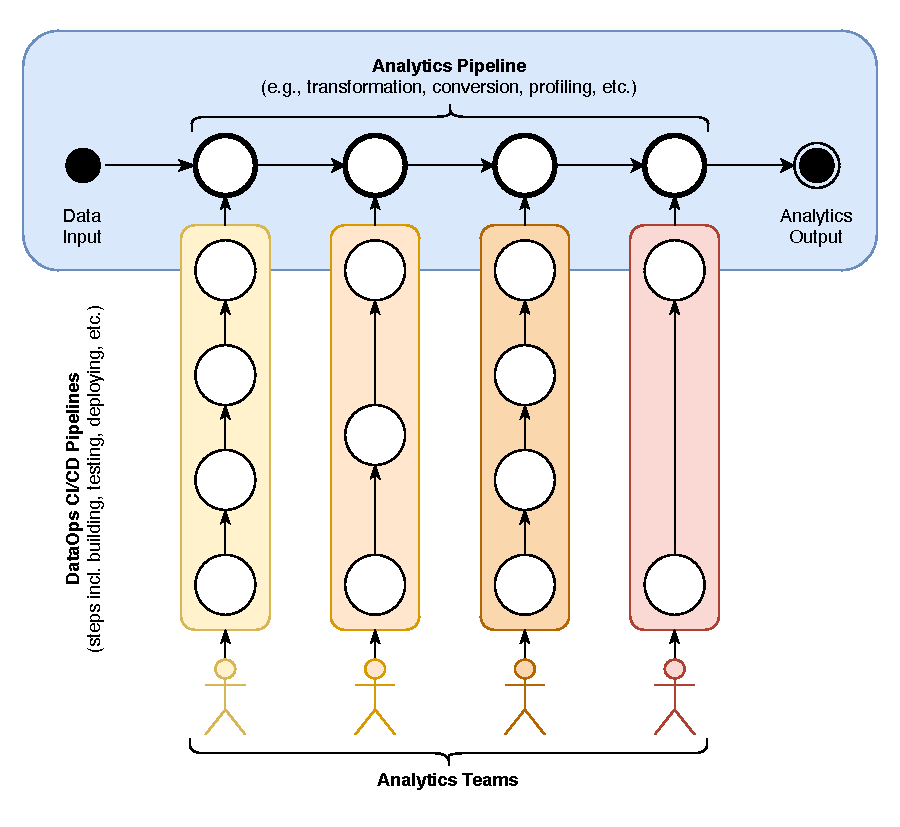
\includegraphics[width=\linewidth]{main-matter/img/2-1-2-pipeline-duality.pdf}
	\caption[DataOps Pipeline Duality]{DataOps Pipeline Duality (per \cite[38\psqq]{Bergh2019})}
	\label{fig:2-pipeline-duality}
\end{figure}

The data analytics (or data operations) pipeline is also called \textit{Value Pipeline} since it is in charge of answering questions through analytical insights \cite[32\psq]{Bergh2019}. Its horizontal representation visualizes its continuous flow. On the contrary, the vertical pipelines, also called \textit{Innovation Pipelines}, represent the DataOps \ac{cicd} pipelines \cite[66]{Schmidt2019}. Whenever a new feature is developed for any stage of the pipeline, a number of preliminary steps is performed before finally deploying the solution into production \cite[33]{Bergh2019}. As with data analytics in general, the design of such pipelines highly depends on the analytics and quality requirements. In the scenario of Figure \ref{fig:2-pipeline-duality}, the individual stages require different \ac{cicd} steps and might also be worked on by different teams within the superordinate project.

As with DevOps, DataOps \ac{cicd} ties in with the project's \acf{vcs}. This allows for collaboration between developers as well as development environment management \cite{Davis2020}. Usually, a developer uses an individual sandbox to make changes to the common source code. This sandbox is a highly isolated environment which can be used without impacting the development process of other developers. It includes the current common source code as well as processes for installing and running all required dependencies \cite[41]{Bergh2019}. When committing a change to the \ac{vcs}, it triggers the corresponding \ac{cicd} pipeline which performs its checks and reports potential issues. Otherwise, the updated source code becomes the new common source code since the deployment into production has been conducted successfully.

Another methodology originating from DevOps is \textit{\ac{iac}}. In a desired automated environment, \ac{iac} also enables automatic creation, provisioning, and re-instantiation of a (cloud) infrastructure \cite[8\psqq]{Chaganti2018} which does not require repeated \acs{ui}-based configuration, etc. This is enabled by programatic configuration of infrastructure resources, settings, as well as applications.

\subsection{Agile Heritage: Fast-Paced, Iterative Development}
One problem within data analytics is that traditionally developed solutions cannot keep up with the demand of changing requirements. The development process is slow such that valuable and time-dependent information cannot be processed on time \cite{Lockner2019}. In software development, agile development mostly replaced traditional waterfall-orientated processes. \textit{Agile} in DataOps context means that development and improvement is iterative and fast-paced. It requires a \ac{mvp} which is continuously improved by means of previously mentioned \ac{spc} and \ac{cicd} processes \cite[19\psq]{Bergh2019}.

    

\section{Introduction to Testing}
	\label{sec:2-testing}
    The previous section introduced areas where testing aspects can be found within DataOps. This section presents the current state of the art for software and data quality testing. Both disciplines will be evaluated and used within the testing framework design process.

\subsection{Why Do We Need Testing?}
In general, software development relies on testing principles to holistically and objectively validate the expected performance of a piece of software. Nowadays, organizations depend on data analytics more than ever \cite{Munawar2011}. \ac{bi} and \ac{dwh} solutions are designed to utilize data for business-required decision making \cite{Souibgui2019}. While these systems are expected to generate value, many companies lose trust in their data analytics because it might be prone to unforeseeable errors \cite{BISurvey.com}. This is because \ac{bi} and \ac{dwh} systems rely on high-quality data in order to provide representative analytics results and business insights \cite{Munawar2011}. Unfortunately, data quality issues of various sorts and manifestations lead to the systems generating false and potentially misleading reports \cite{Munawar2011}\cite{Freudiger2014}\cite{Redman2016}. Testing the solution for its expected performance at various analytics steps might help solve the underlying issues or even exhaust them completely. 

From a pure software perspective, it is desired that the solution does not break or crash during analytics performance for an unforeseeable reason. Applicable software tests could recognize such issues prior to production deployment, reducing or completely removing crucial bugs inside the software \cite[105\psqq]{ORegan2017}. \\\

As previously mentioned in Section \ref{sec:2-1-devops}, the pipeline duality ensures continuous flow of both production-grade data analytics as well as improvement and enhancement of the solution. Both pipelines require individual testing measures. This is referred to as \enquote{The Duality of [DataOps] Testing.} \cite[40\psqq]{Bergh2019}

\subsection{Value Pipeline: Data Quality Testing} \label{sec:2-2-value-pipeline}
Since the Value Pipeline is in charge of the business-critical analysis of various data, the solution-in-use must guarantee the recognition and handling of data quality issues prior, during, and after each individual processing step by means of its \ac{spc} capability. In other words, while the underlying analytics software is static, the variance of data is arbitrarily large and needs to be handled properly \cite[p. 47, fig. 17]{Bergh2019}. In order to define this kind of event handling, unified data quality dimensions are required.

The \ac{dama} in the United Kingdom defined \enquote{The Six Primary Dimensions for Data Quality Assessment} in 2013 \cite[7\psqq]{Askham2013}. They consist of:

\begin{description}
	\item[Completeness] describes the proportion of the stored data against the potential of being \textit{complete} by means of a use-case-specific completeness definition \cite[8]{Askham2013}\cite{Shen2019}.
	\item[Uniqueness] is achieved when each unique data record only exists once inside the entire database at hand \cite[9]{Askham2013}.
	\item[Timeliness] is the degree to which data represents the reality from the required point in time \cite[10]{Askham2013}.
	\item[Validity] describes a data item corresponding to its expected (and therefore, pre-defined) format, schema, syntax, etc. This definition should also include a range of expected or acceptable variation thresholds \cite[11]{Askham2013}. Testing for data schematics is one processes which allows for definitive objective differentiation between good and bad data \cite{Schieferdecker2012}.
	\item[Accuracy] is the degree to which data \textit{correctly} describes the actual object or event existing in the real world \cite[12]{Askham2013}.
	\item[Consistency] describes the absence of difference when comparing multiple representations of the same real-life object against its actual definition \cite[13]{Askham2013}.
\end{description}

It can be seen that the areas of data quality are mostly covered when data complies with the corresponding data governance definitions \cite{Schieferdecker2012}. These definitions build the foundation for a valid testing framework.

In practice, checks based on these dimensions have to be embodied inside the data analytics solution. Based on mentioned, use-case-specific requirements, a data flow can be checked by means of those dimensions, leading to recovery measures inside the system, or an intentional system failure with appropriate error reporting.

\subsection{Innovation Pipelines: Software Testing} \label{sec:2-2-innovation-pipeline}
Section \ref{sec:2-1-devops} describes the Innovation Pipelines as DataOps-specific \ac{cicd} pipelines. Apart from the build and deployment process, a major part of these pipelines is represented by software testing. Whenever a developer intends to update the codebase, a number of tests of various levels is conducted, visualized in the pyramid graphic in Figure \ref{fig:2-testing-pyramid} below.

Depending on the type of software, the types and levels of testing can vary. For data analytics solutions with \acp{ui} outside their scope, the three foundational levels suffice.

\begin{figure}[h!]
	\centering
	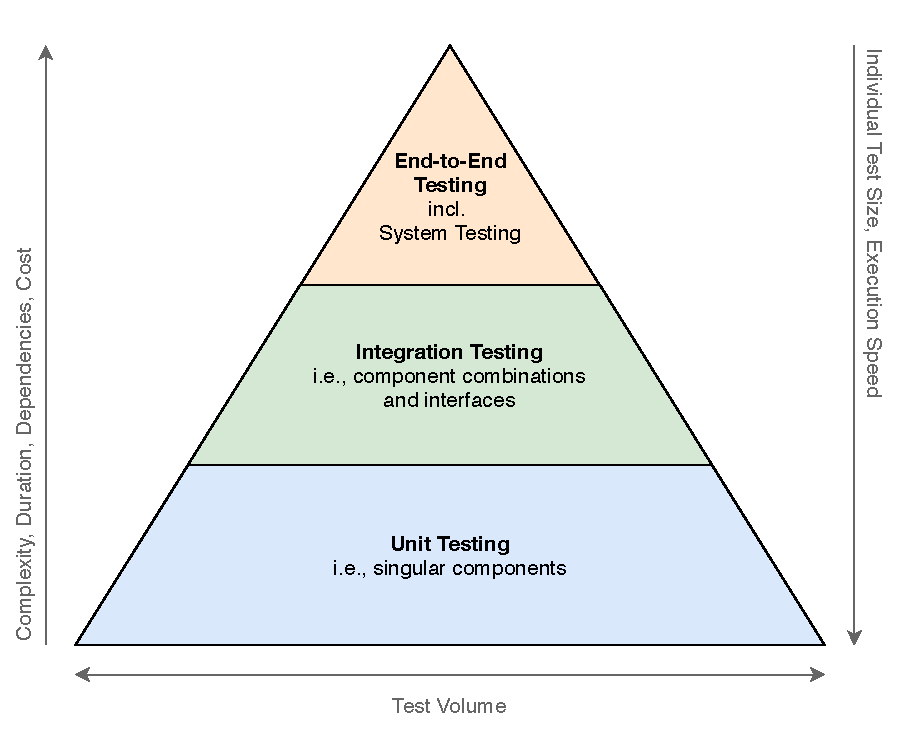
\includegraphics{main-matter/img/2-2-3-testing-pyramid.pdf}
	\caption[Software Testing Level Pyramid]{Software Testing Level Pyramid (per \cite{devops-google})}
	\label{fig:2-testing-pyramid}
\end{figure}

\newpage



\begin{description}
	\item[Unit Tests] take individual components (i.e., \textit{units}) from the source code and check their behavior. Unit tests are pieces of code that invoke the chosen test unit and compare its actual result with the expected outcome \cite[sec. 1]{Osherove2013}. They are characterized as granular, thus highly voluminous, repeatable, isolated, and idempotent \cite[sec. 2]{Osherove2013}.
	\item[Integration Test] verify that multiple combined units are working together as expected. They focus on testing of interfaces that connect singular components \cite[66]{Mahfuz2016}. Integration tests are performed in a less isolated environment, resulting in more outside dependencies \cite[sec. 3]{Osherove2013}.
	\item[End-to-End Tests] describe the highest level of software testing \cite[67]{Mahfuz2016}. For the sake of simplicity, system tests are treated as a part of end-to-end tests within this work. End-to-end tests are performed under a (close-to) deployment situation. This creates an idealized real-life scenario. Thus, end-to-end testing is the least isolated level and serves as the final test stage before actual deployment. \cite[67]{Mahfuz2016}.
\end{description}



Those three layers represent the \textit{Fuctional Testing} type since they are built based on the functional requirements of a software solution \cite[69]{Mahfuz2016}. Its counterpart, \textit{Non-Functional Testing}, covers aspects like load, performance, security, etc. \cite[70]{Mahfuz2016}.

In traditional DevOps \ac{cicd} testing, the testing pyramid is seen as the ideal testing design structure \cite{devops-google}. It generally aims for discovering errors at the earliest testing stage possible, leading to a high volume of unit tests \cite{Vocke2018}.

Apart from that, other testing methods can be applied to each testing layer. \textit{Smoke Tests} are a subset within the entire test suite that cover core functionality required for the solution to \textit{just} run. Such tests can help to recognize the complexity of a software issue \cite[sec. 5]{Tarlinder2016}. Conducting \textit{Regression Tests} is also important. They aim to uncover errors with pre-existing components when other components were newly included, changed, or removed \cite[70]{Mahfuz2016}\cite{Mathur2013}. This is especially crucial with data analytics solutions since historic data still needs to be processable after updating the analytics engine \cite{Shen2019}. To achieve regression testing in practice, unit tests can be written in a more abstract manner and re-run for the entire software solution, requiring older unit tests still to pass \cite{Mathur2013}.
\\\

Putting everything into DataOps perspective, the Innovation Pipelines need to cover source code changes of the analytics solution. These \ac{cicd} pipelines need to embody traditional software tests to verify the correct behavior of the application. This also includes testing the \ac{spc} capability of the given solution \cite{DataKitchen2020}. For that reason, pathological test data needs to be provided that is able to invoke a majority of realistic events during the analytics process \cite[42]{Bergh2019}. In case of tests failing, the corresponding \ac{cicd} Innovation Pipeline can report the issue back to the developer, allowing for further understanding and correction. These tests are expected to invoke the majority of outcome possibilities, leading to a high test coverage and correct performance validation \cite{DataKitchen2020a}.

Considering DevOps testing (as opposed to the currently discussed DataOps testing) which is expected not to be data-driven, there exist many similarities to the Innovation Pipeline testing process. In general, the features of the solution need to be tested and validated based on their desired functionality. However, DataOps introduces a highly data-focussed testing process, requiring data governance consideration, test data management, etc.. Plus, it is expected to set different priorities in testing because of this data aspect. These priorities as well as further similarities and differences between DevOps and DataOps testing are discussed and expected to be deduced in the \nameref{chap:solution-evaluation} chapter.







	\chapter{Actual State Analysis}
		\label{chap:actual-state-analysis}
		%===========================================================================
%	III. Actual State Analysis
%===========================================================================

As stated in the \nameref{chap:introduction} chapter, the project is conducted based on a preexisting data pipeline solution where DataOps is to be enabled, including a holistic DataOps testing framework. This chapter performs an actual state analysis, describing the superordinate data analytics use case as well as the data pipeline specification prior to the project. The resulting aspects will then be used for the testing framework specification and reimplementation process.

\section{General Information}
The data pipeline at hand is four-stage pipeline that creates a \acf{mba} for \ac{bi} and reporting purposes. \ac{mba} is one of the key techniques used by retail companies to uncover associations and patterns within item purchases. It works by looking for combinations of items that occur together frequently in transactions \cite[1]{Chen2005}. The specific \ac{mba} performed at the end of this data pipeline provides two kinds of information. First, it describes item sets that are frequently purchased together. Specifically, the higher the \textit{support} of an item set, the higher the probability that these items are purchased together. The \textit{Apriori} algorithm is a widely used method to accomplish this \cite[12\psq]{Wu2008}. Second, the \ac{mba} calculates other association metrics (i.e., \textit{confidence} and \textit{lift}) of the item sets, allowing for backed decision-making with regard to marketing campaigns, inventory stock-up, etc.

\acp{mba} are based on a large amount of \acf{pos} data. This data needs to be integrated by means of the analytics engine requirements in order to be used for \ac{mba} purposes.
\newpage
\section{Analytics Solution Components}
The data pipeline consists of various infrastructural and technical components. This also includes the input and output formats of the analyses. These components are described in the following.

\subsection{\acs{mba} Engine: Python Library \texttt{mlxtend}}
The Python library \texttt{mlxtend} provides functions that are required for conducting the previously described \ac{mba}. \texttt{mlxtend.apriori} conducts the analysis of frequent item sets by means of their support. These are used for the second step, where \texttt{mlxtend.association\_rules} is leveraged to calculate confidence and lift metrics \cite{mlxtend} for all item sets with support > 5\%. Currently, the resulting associations are filtered such that only those with a high lift (> 6) and high confidence (> 0.8) are provided. The result is a Microsoft Excel spreadsheet document which lists all analytically promising item sets.

For better distinction between the actual association of the products, the \ac{mba} engine performs two analyses. Technically, they perform identically but the first analysis only considers items that are classified as food. The second analysis performs by only looking at non-food items. Thus, the analysis does not take cross-category associations into account, as they might be random and complicated to take advantage of.

The \texttt{mlxtend} library works with so-called data frames which are typically managed by another Python library, \texttt{pandas} \cite{pandas}. The \ac{mba} algorithms require a data frame that flags what kinds of sub-categories of products (both food and non-food items) were purchased in every considered transaction. Thus, to provide these pieces of information, \texttt{pandas} requires an input of semi-structured data \cite{pandas} where the following requirements are satisfied:

\begin{itemize}
	\item each individual transaction can be identified: \texttt{InvoiceNo} attribute for each purchase
	\item each individual item is sub-categorized: \texttt{Description} attribute for each purchase
	\item each individual item is categorized (food or non-food): \texttt{ItemType} attribute for each purchase
	\item each individual purchase shows if and how much of an item was purchased: \texttt{Quantity} attribute
\end{itemize}

All these requirements can be satisfied by providing a single \ac{csv} file which contains an arbitrary number of transactions. Based on the transaction information, the \ac{mba} is conducted.


\subsection{Input Data: \textit{\acs{arts} \acs{pos}Log 6} Standard}
Transaction data is usually provided to the customer through a receipt that is printed out at the register. This data can also be leveraged for \ac{mba}. Since multiple registers across multiple branches of a retail company produce a large number of individual receipts every day, the format of those \ac{pos} data needs to be unified. Additionally, the data needs to be centralized such that cross-branch \acp{mba} are possible.

A widely used \ac{pos} standard is the \textit{\ac{pos}Log 6} standard by the \ac{arts}. It is used by many established register systems. It is saved in \ac{xml} format and contains the same information that is usually provided on a print-out receipt \cite{poslog}, i.e., general transaction information (e.g., name and address of retail branch, cashier's name, currency) as well as information on each item purchased (category, brand name, quantity, price, etc.). The provided information allows to find out the required attributes for \ac{mba}.

An exemplary \ac{xml} code snippet in \ac{pos}Log format for the current solution looks as follows:

\begin{longlisting}
	\inputminted{xml}{main-matter/src/3-poslog.xml}
	\caption{Sample \acs{pos}Log \acs{xml} File}
	\label{src:3-poslog}
\end{longlisting}

\subsection{Data Location: \textit{\acs{aws} \acs{s3} Data Bucket}} \label{sec:3-2-data-lake}
In a real-life retail scenario, the individual \ac{pos} data of each branch could be consequently uploaded to the branches' data infrastructure. Each day at end of business, this data needs to be provided to the global \ac{mba} engine. This is why the data is compressed into a single ZIP archive, identified by branch name and date stamp, and uploaded to the landing zone of the retail company's global data lake. This data lake is realized with an \ac{aws} \ac{s3} data bucket, a server-less data storage solution \cite{s3}. The data lake structure can be seen in Figure \ref{fig:3-data-lake}.

\newpage

\begin{figure}[h!]
	\centering
	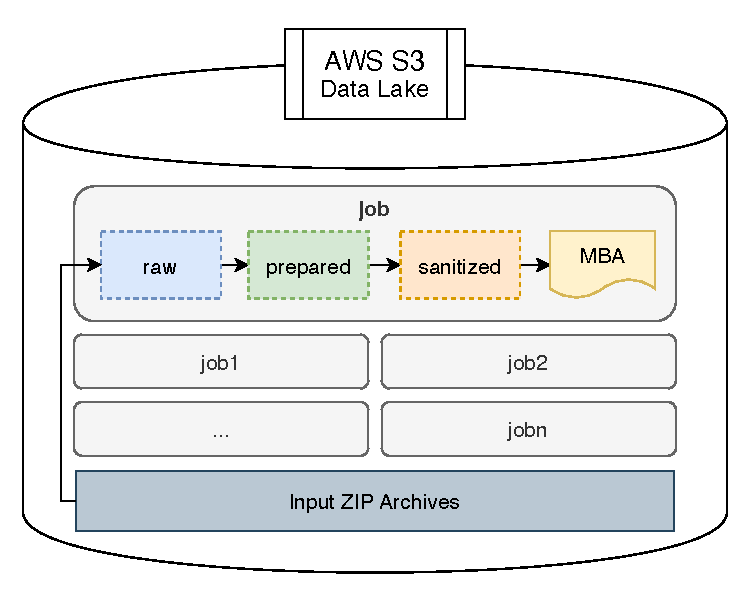
\includegraphics[width=0.67\linewidth]{main-matter/img/3-data-lake.pdf}
	\caption{Preliminary Data Lake Structure}
	\label{fig:3-data-lake}
\end{figure}

For the data analytics pipeline which integrates the data and performs the actual \ac{mba}, the landing zone of production-grade data (as described in the previous paragraph) is considered the entry point. It receives the previously mentioned \ac{pos}Log ZIP archives. It also contains individual job areas that contain all analytics results, e.g., an \ac{mba} every day after receiving new data. Each job area is again divided into sub-areas that are used as intermediate destinations for the individual data pipeline stages, while the resulting \ac{mba} Excel spreadsheet file is uploaded to the root of its job area.

\subsection{Centralized Data Processing Engine: \textit{\acs{aws} Athena} Serverless \acs{sql} Database}

It is desirable that a global \ac{mba} engine performs the analysis rather than every branch performing their own analyses since this might lead to inconsistencies between the individual results. Therefore, the data lake is not only used for storage purposes, but is rather the actual area where the analysis is performed based on the contents in its raw zone. Considering structure, all \ac{pos} data across all branches is expected to be identical, which means that all data can be normalized and synthesized in the same way, allowing the data to be ingested into a relational database table for querying purposes.

\ac{aws} Athena makes use of the \ac{s3} data lake and does not require additional data storage resources. It rather considers a specific area of the \ac{s3} bucket its data source and can query against it using traditional \ac{sql} \cite{athena}. The query results are represented in \ac{csv} format that can be used by the \ac{mba} engine to perform its analyses.

The query for the information required by the MBA looks as follows:

\begin{listing}[H]
	\inputminted{sql}{main-matter/src/3-athena-query.sql}
	\caption{\acs{sql} Query for Required \acs{mba} Information}
	\label{src:3-athena-query}
\end{listing}

This yields an output of the following format:
\begin{table}[h!]
	\centering
	\begin{tabular}{r!{\vrule width 1pt}l|l}
		\textbf{Attribute}      & \textbf{Data Type}  & \textbf{Corresponding \acs{json} Attribute}  \\ \ChangeRT{1pt}
		\textbf{\texttt{SequenceNumber}} & \texttt{bigint}     & \texttt{SequenceNumber}               \\ \hline
		\textbf{\texttt{Description}}    & \texttt{string}     & \texttt{ItemCategory}                 \\ \hline
		\textbf{\texttt{ItemType}}       & \texttt{char} (\texttt{F}/\texttt{N}) & \texttt{ItemID} (first character)     \\ \hline
		\textbf{\texttt{Quantity}}       & \texttt{int}        & \texttt{Quantity}                    
	\end{tabular}
	\caption{\acs{csv} Output Format}
	\label{tab:3-csv-format}
\end{table}

Using an entire external service (i.e., \ac{aws} Athena) might appear to have a high overhead but could be leveraged especially in situations where the \ac{mba} input requires different data. In that case, only an \ac{sql} query would need to be updated, as opposed to the entire source code of one or multiple stages of the pipeline. In case the MBA does not change its requirements, it might be possible to handle the \ac{xml}-to-\ac{csv} conversion and reduction internally. The current solution applies \ac{aws} Athena for simplicity reasons.

\section{Data Pipeline} \label{sec:3-data-pipeline}
The goal of the data pipeline is to integrate the input data (i.e., the \ac{pos}Log \ac{xml} files) and prepare the required accumulated, \ac{csv}-formatted data for the actual \ac{mba}. This process is divided into three preparatory data integration stages and followed by the fourth and final \ac{mba} stage.

In theory, a data pipeline can be understood as a \ac{dag}, since it defines a specific flow direction as well as a beginning and an end of one analytics period. The pipeline \ac{dag} at hand is technically encapsulated inside the \textit{Apache Airflow} workflow software, residing on a \ac{aws} \ac{ec2} virtual server instance. It makes use of \acp{dag} to define, manage, and operate (analytical) workflows. Airflow is Python-driven and provides a \ac{ui} for real-time monitoring purposes \cite{airflow}, which makes it suitable for data analytics processes. It is important to mention that, currently, Airflow does not only orchestrate the analysis, but rather performs it. All analytics scripts are directly written into Airflow. The terms \textit{pipeline} and \textit{\ac{dag}} can be used interchangeably in the current state of the analytics solution. Its general structure is presented in Figure \ref{fig:3-data-pipeline} below.

\begin{figure}[h!]
	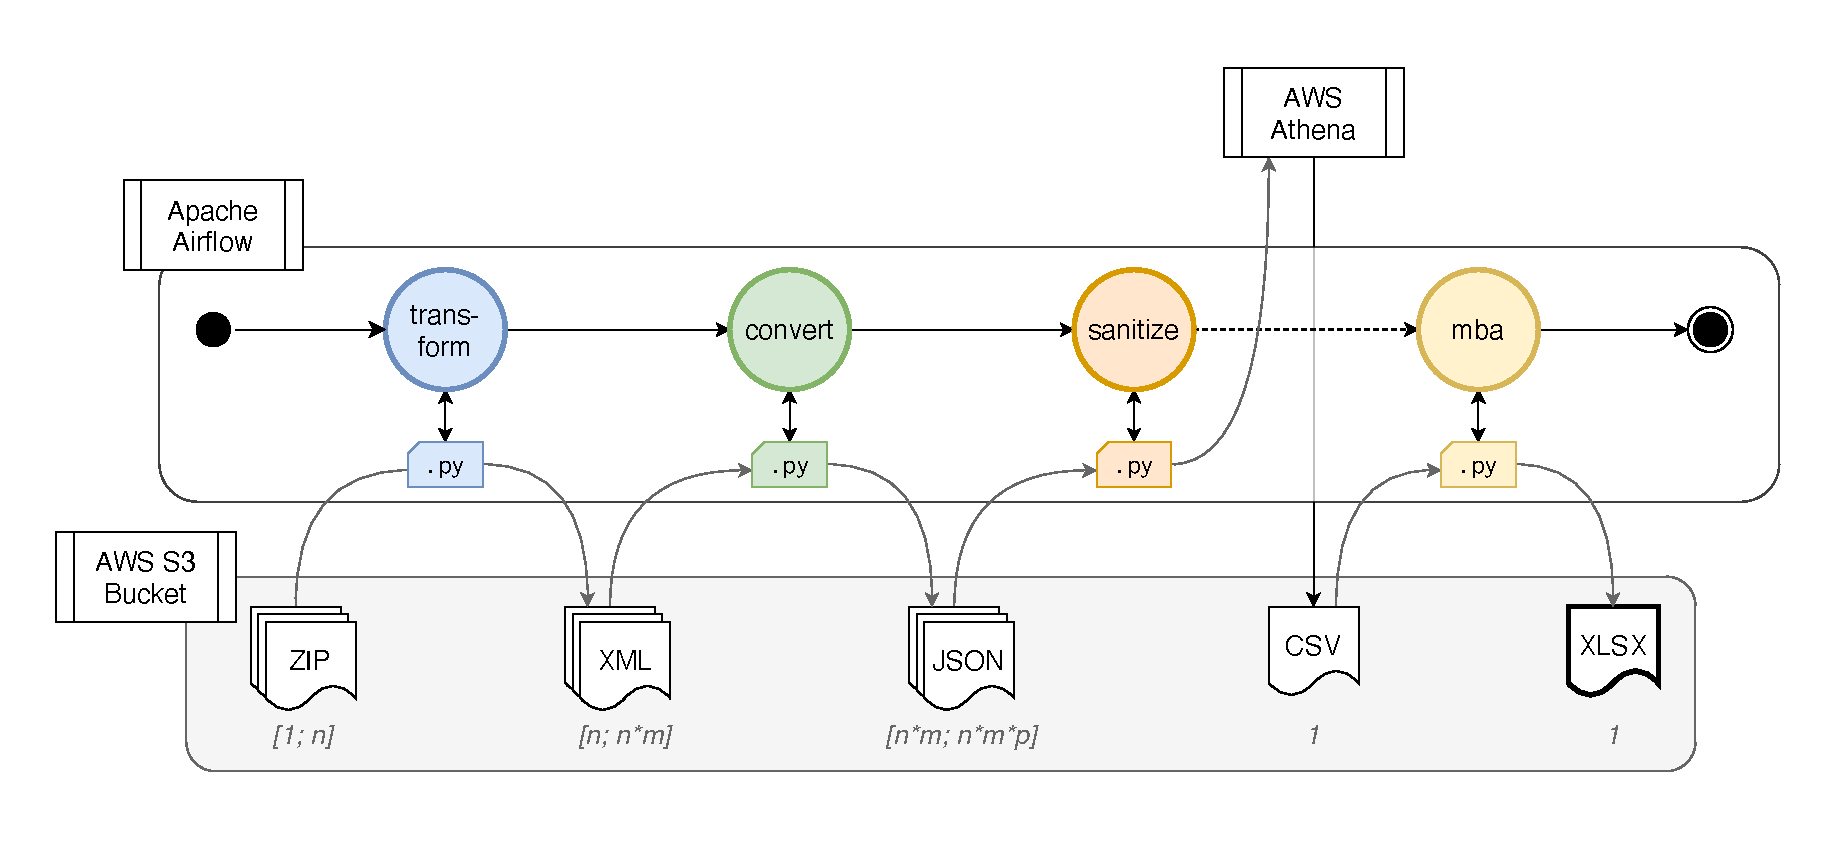
\includegraphics[width=\linewidth]{main-matter/img/3-3-data-pipeline.pdf}
	\caption{Data Pipeline Overview}
	\label{fig:3-data-pipeline}	
\end{figure}

As shown in Figure \ref{fig:3-data-pipeline}, the Transformation Stage scans the pre-defined data lake landing zone for ZIP archives. It decompresses the ZIP archives and loads all \ac{xml} files into a designated raw-file directory of the job-specific data lake space. The Conversion Stage takes the resulting data and prepares it for a server-less database integration, realized with \ac{aws} Athena. The Sanitization Stage queries the resulting table for the attributes required by the \ac{mba} engine. The query result is exported in \ac{csv} format and provided to the \ac{mba} engine, which performs the analysis in its designated \ac{mba} Stage, which represents the final stage of the data pipeline.

All communication between the analytics solution and the various \ac{aws} resources is done via the \ac{aws} Python \ac{sdk} \texttt{boto3} \cite{boto3}.

\newpage

\subsection{Transformation Stage}
Figure \ref{fig:3-transform} visualizes the Transformation Stage.

\begin{figure}[h!]
	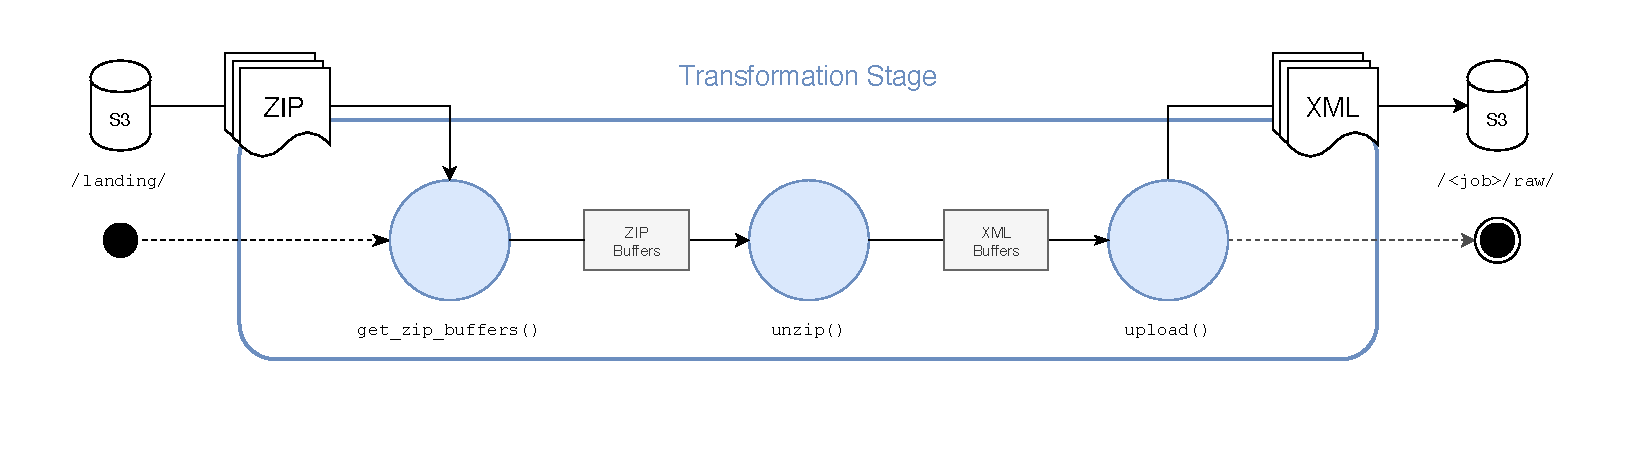
\includegraphics[width=\linewidth]{main-matter/img/3-3-1-transform.pdf}
	\caption{Transformation Stage of the Data Pipeline}
	\label{fig:3-transform}	
\end{figure}

The archived \ac{xml} data needs to be decompressed such that its contents can be read out and analyzed. In order not to contaminate the landing zone of the data lake, the data is simply decompressed and uploaded to a raw-file directory within the designated job data lake space. The \ac{xml} data is nested, which is not suited for the direct integration into a relational database table, which is why the data needs to be converted in the next stage.

\subsection{Conversion Stage} \label{sec:3-3-conversion}
Figure \ref{fig:3-convert} visualizes the Conversion Stage.

\begin{figure}[h!]
	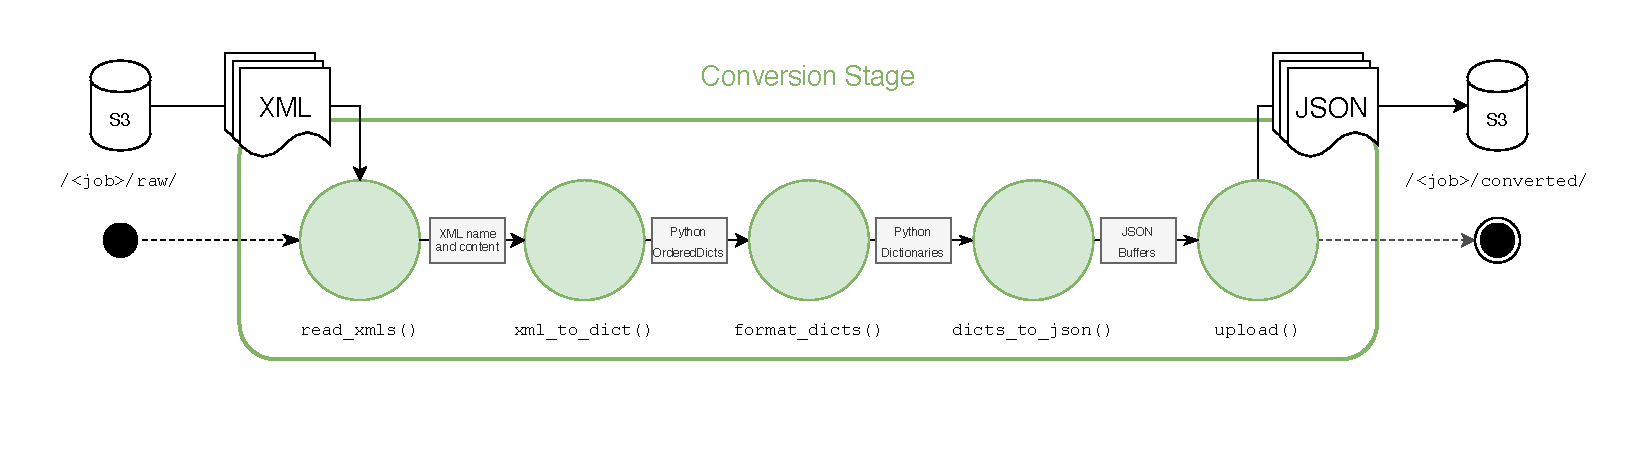
\includegraphics[width=\linewidth]{main-matter/img/3-3-2-convert.pdf}
	\caption{Conversion Stage of the Data Pipeline}
	\label{fig:3-convert}	
\end{figure}

The \ac{xml} files contain transaction-level information where the individual purchases are nested into. The \ac{mba} engine requires purchase-level information with a transaction reference which means that the \ac{xml} data needs to be redundantly converted. The resulting data should still contain transaction information, but a single data entity needs to provide information on a single purchase within the referenced transaction and shall not be nested.

Before this conversion can take place, the \ac{xml} data needs to be made processable in Python. Here, the \texttt{xmltodict} library is leveraged. The resulting Python dictionaries reflect the structure of the \ac{xml} file. To achieve the goal of purchase-level dictionaries, each purchase in a dictionary creates its own dictionary and also gets all transaction information provided. This process is visualized in Figure \ref{fig:3-convert-process}.

\begin{figure}[h!]
	\centering
	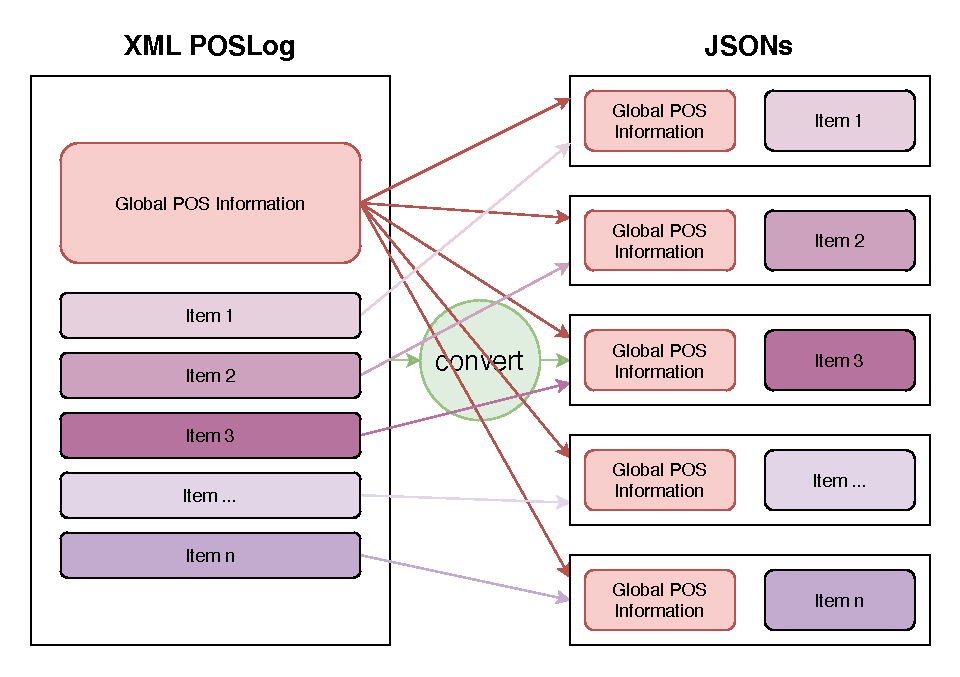
\includegraphics[width=0.67\linewidth]{main-matter/img/3-convert-process.pdf}
	\caption{Conversion of Nested \acs{pos}Log \acs{xml} Files}
	\label{fig:3-convert-process}
\end{figure}

In simple terms, each new dictionary can be seen as a receipt for a single purchase since it contains all global transaction information as well as sale information for a single item.

The final step of this stage is to provide the data in a format that can be queried against using \ac{aws} Athena \ac{sql} queries. Per its documentation, \ac{json} is a supported data format \cite{athena}. Thus, each dictionary is exported as its own \ac{json} file to a prepared-file directory within the designated job data lake space. An example output \ac{json} file can be seen below.

\begin{longlisting}
	\inputminted{json}{main-matter/src/3-json.json}
	\caption{Sample Converted Single-\acs{pos} \acs{json} File}
	\label{src:3-json}
\end{longlisting}

The query itself is performed in the next stage.

\subsection{Sanitization Stage}
Figure \ref{fig:3-sanitize} visualizes the Sanitization Stage.

\begin{figure}[h!]
	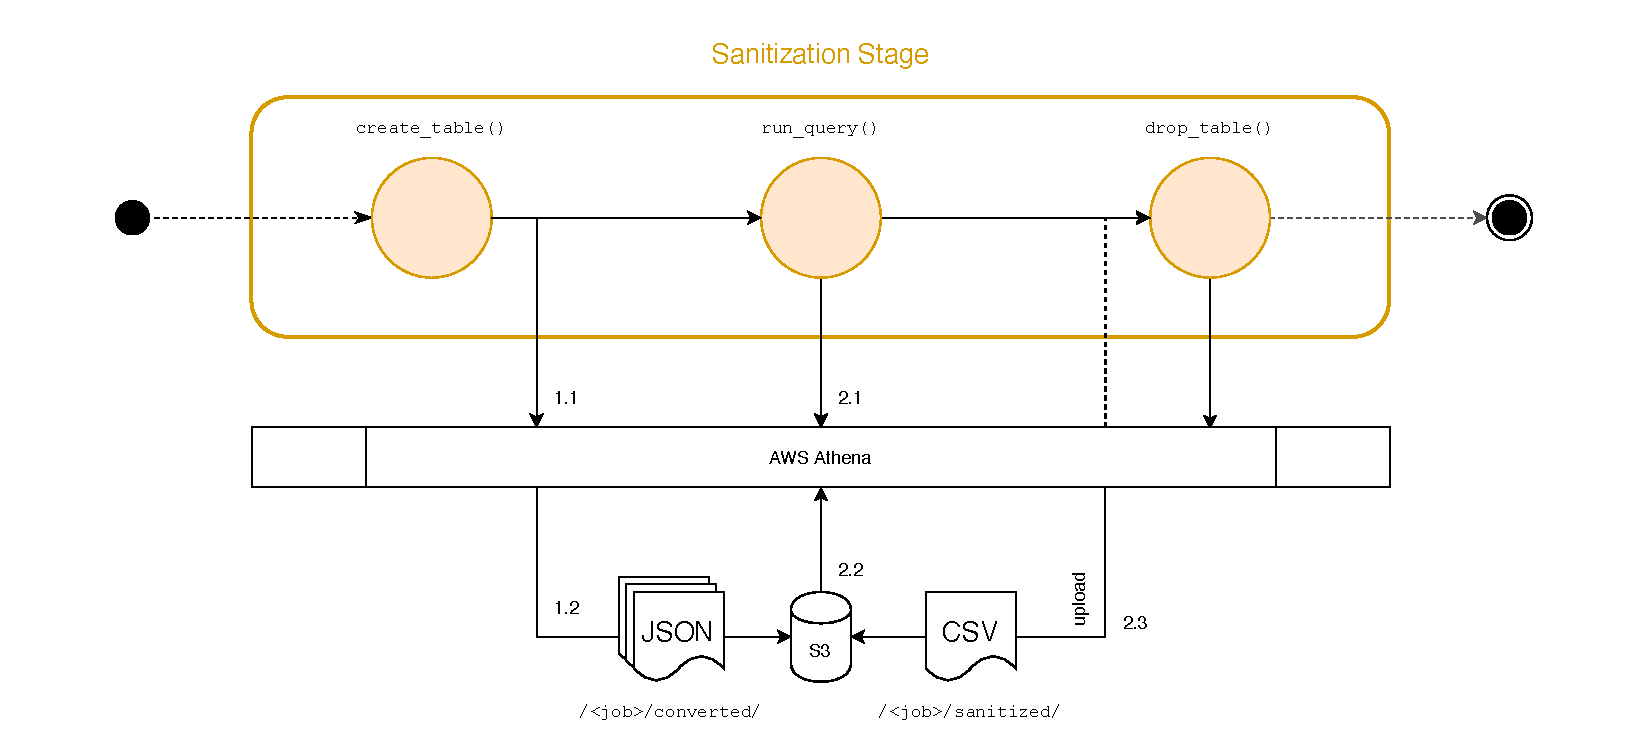
\includegraphics[width=\linewidth]{main-matter/img/3-3-3-sanitize.pdf}
	\caption{Sanitization Stage of the Data Pipeline}
	\label{fig:3-sanitize}	
\end{figure}

The currently provided \ac{json} files contain a significant amount of information which is not required for \ac{mba}. The data needs to be sanitized to only the required attributes for \ac{mba} and exported in \ac{csv} format.

Since each individual \ac{mba} has its own designated space in the data lake, the relational database table for each MBA needs to be created with its appropriate \ac{json} file location. Thus, Athena \ac{ddl} is used to create the table and insert each \ac{json} file as a row into the table.

After the table is populated, the Athena \ac{sql} query for \texttt{InvoiceNo}, \texttt{Description}, \texttt{ItemType}, and \texttt{Quantity} (cf. Source Code Excerpt \ref{src:3-athena-query}) results in the representation that is needed by the \ac{mba} engine. This query result is exported to the sanitized-file directory of the job-specific data lake space. For the sake of a clean environment, the previously created table is dropped. The generated \ac{csv} file can now be used for \ac{mba}.

\subsection{\acs{mba} Stage}
Figure \ref{fig:3-mba} visualizes the \ac{mba} Stage.

\begin{figure}[h!]
	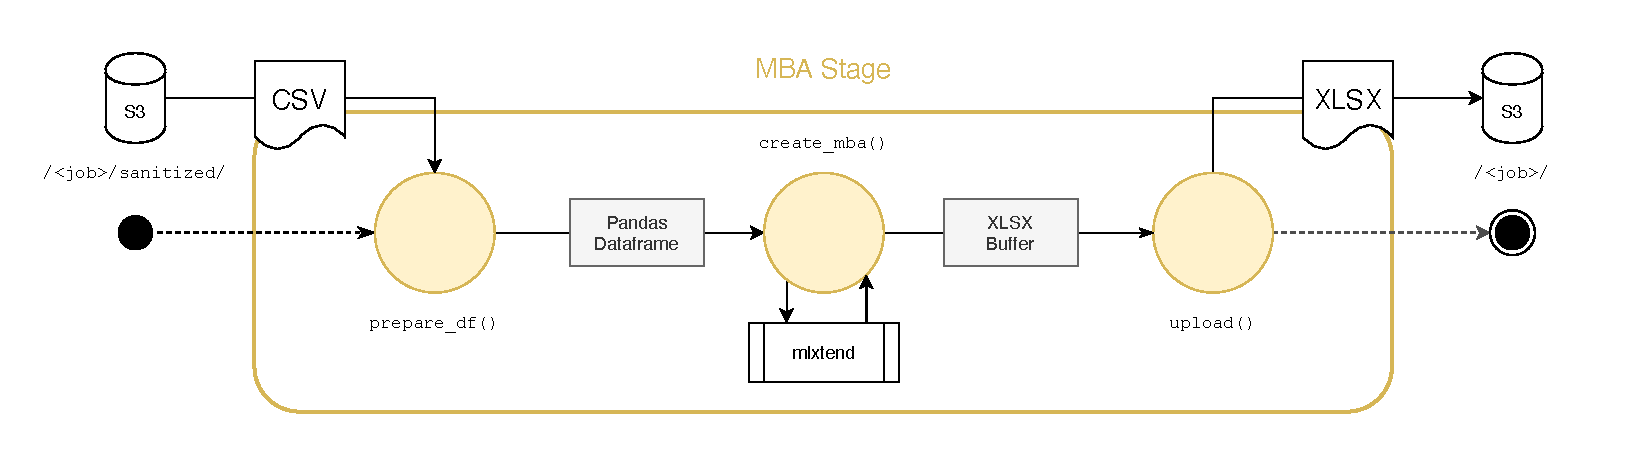
\includegraphics[width=\linewidth]{main-matter/img/3-3-4-mba.pdf}
	\caption{\acs{mba} Stage of the Data Pipeline}
	\label{fig:3-mba}	
\end{figure}

As mentioned in its own section, the \ac{csv} file is provided to the \ac{mba} engine. In case the data is not in correct order (horizontal or vertical, respectively), it is reordered in the process of creating the \texttt{pandas} data frame. \texttt{apriori} is applied on the data frame, which is then used to determine \texttt{association\_rules}. The \texttt{Quantity} attribute of the CSV file provides information on which items (i.e., \texttt{Description}s) where purchased in a transaction (identified by \texttt{InvoiceNo}), separated by \texttt{ItemType} \texttt{F} (i.e., food) and \texttt{N} (i.e., non-food). Both the food and non-food data frames and association rules need to be exported to a single Excel spreadsheet file. This functionality is also covered by \texttt{pandas} \cite{pandas}. This file is finally uploaded to the root directory of the current analysis job data lake space. At this point, one \ac{mba} data pipeline process is finished. 


\section{Comparison to Target Requirements}
From an infrastructure point of view, the preliminary solution meets the requirement of being implemented by means of \ac{aws} cloud services. On the contrary, the current architecture design is not server-less. More specifically, all analytics steps are performed on the same Airflow instance, resulting in bad scalability and undesired analytical isolation (cf. Figure \ref{fig:3-data-pipeline}). Additionally, since some steps inside the pipeline might have different performance requirements, the server-driven architecture could lead to bottlenecks for some stages and to overhead for others.

From a DataOps perspective, the solution at hand lacks fundamental implementation of state-of-the-art methodologies, e.g. \ac{vcs} support, \ac{cicd} automation, etc. These aspects need to be covered, taking the use case circumstances into consideration. Developing the solution needs to be done in individual, isolated environments in order not to contaminate the production-grade environment as well as other developers' environments within the project. This can be achieved by \ac{vcs} enablement. Additionally, since each pipeline stage is expected to be developed and maintained by different developers, the individual stages could have different requirements for their \ac{cicd} automation. Therefore, four individual DataOps \ac{cicd} pipelines need to be implemented by applying the different needs for every stage.

Finally, the current solution is entirely untested. This includes the absence of validating software tests as well as data quality checks within the solution. A general testing framework applied on the use case data definition and governance is required. This framework needs to be designed before it can be embedded inside the future DataOps processes of the solution.		

	\chapter{Testing Framework Design}
		\label{chap:testing-framework}
		%===========================================================================
%	IV. Testing Framework Design
%===========================================================================

The creation of a DataOps testing framework aims to assure the data and software quality requirements of a solution. In general, based on the findings from Section \ref{sec:2-testing}, the following design process of such a framework is proposed:

\begin{enumerate}
	\item Include data quality checks within the solution at hand based on pre-defined data requirements or data governance specifications.
	\item Define test data suites that invoke the data quality checks, resulting in both positive and negative outcomes.
	\item Create automated tests for the solution that make use of the test data suites to verify that the data quality and solution performance requirements are met. These tests will run whenever a new version of the solution is about to be deployed into production.
\end{enumerate}

This chapter takes these steps, elaborates on them, and applies the project's \ac{mba} data pipeline solution on the process. It aims to provide a guideline for designing DataOps testing based on a given scenario. For the desired pilot demonstration, the definition of a testing framework for one specific stage within the data pipeline is sufficient. The Conversion Stage of the \ac{mba} data pipeline is suited for this task since it prepares the Athena database integration of raw \ac{pos}Log data. This includes a variety of data transformation and processing, and thus, is prone to data quality issues throughout the entire flow of the stage.

\section{Data Quality Check Design}
In order to check for data quality issues within a data flow, it is important to understand the different steps the given solution performs during its flow. As stated in Section \ref{sec:2-2-value-pipeline}, this also includes the inspection of the raw input data and the final processed output data. In a multi-stage environment, it is also important to consider the required input for the next pipeline stages, in this case, the Sanitization Stage.

\subsection{Conversion Stage Data Governance Review}
Input and output data requirements should be defined by the use case's data governance. In the Conversion Stage's case, the input data should consist of one or multiple \ac{pos}Log \ac{xml} files (cf. Section \ref{sec:3-3-conversion}). The input data is also expected to be named in a unified format which contains retail branch store information, date information, as well as the identification number of the receipt (cf. Section \ref{sec:3-2-data-lake}). The data needs to originate from the \texttt{raw} subarea within the specific analytics job area inside the data lake (cf. Figure \ref{fig:3-data-lake}) The output data needs to be provided in \ac{json} file format, where one \ac{pos}Log \ac{xml} file yields one or multiple \ac{json} \ac{pos} files, containing global receipt as well as single-purchase information (cf. Section \ref{sec:3-3-conversion}), depending on the number of items from the source \ac{pos}Log file. Thus, the data values of the individual files do not change but get rather split up and reformatted. For the output data, a similar unified naming format, including the order of purchases from the original \ac{pos}Log file, is also required. The data destination is the \texttt{prepared} sub-area within the specific analytics job area inside the data lake. This data governance information can now be summarized in Table \ref{tab:4-data-gov-convert}:

\begin{table}[h!]
	\centering
	\begin{tabular}{r!{\vrule width 1pt}l!{\vrule width 0.5pt}l}
\textbf{}                & \textbf{Input Data}                                                                                           & \textbf{Output Data}                                                                                                                        \\ \ChangeRT{1pt}
\makecell[r]{\textbf{Data}\\\textbf{Format}}     & \makecell[l]{\texttt{\ac{xml}}\\with \ac{pos}Log formatting}                                                                          & \makecell[l]{\texttt{\ac{json}}\\with defined single-\ac{pos} formatting}                                                                                    \\ \ChangeRT{0.5pt}
\makecell[r]{\textbf{Data}\\\textbf{Amount}}     & \makecell[l]{$n > 0$}                                                                                     & \makecell[l]{$m \cdot n \geq n$ \\ where $m > 0$ is the number of individual \\ items for each \ac{pos}Log file $1$ to $n$}                          \\ \hline

\makecell[r]{\textbf{File}\\\textbf{Naming}}     & \makecell[l]{\texttt{\textless{}store-id\textgreater{}\_\textless{}date\textgreater{}\_} \\ \texttt{pos\textless{}no\textgreater{}.xml}} & \makecell[l]{\texttt{\textless{}store-id\textgreater{}\_\textless{}date\textgreater{}\_}\\ \texttt{pos\textless{}no\textgreater{}\_\textless{}sq\textgreater{}.json}} \\ \hline


\makecell[r]{\textbf{Location}\\\textbf{Format}} & \makecell[l]{\texttt{s3://\textless{}bucket-name\textgreater{}/} \\ \texttt{\textless{}job-id\textgreater{}/raw}}                        & \makecell[l]{\texttt{s3://\textless{}bucket-name\textgreater{}/} \\ \texttt{\textless{}job-id\textgreater{}/prepared}}                  
\end{tabular}
	\caption{Conversion Stage Data Governance Specification Summary}
	\label{tab:4-data-gov-convert}
\end{table}

The corresponding format examples have already been provided in Source Code Excerpt \ref{src:3-poslog} and Source Code Excerpt \ref{src:3-json}.

As previously depicted in Figure \ref{fig:3-convert}, the Conversion Stage runs through the following data-focussed tasks to achieve the conversion:

\begin{enumerate}
	\item Take the data from the \ac{s3} bucket and read its (binary) contents.
	\item Map those contents to \texttt{OrderedDict}s using Python's \texttt{xmltodict} library
	\item Remove nesting from the dictionaries by reformatting each \texttt{OrderedDict} to multiple, single-\ac{pos} standard Python dictionaries
	\item Export each single-\ac{pos} dictionary to \ac{json} (binary) format
	\item Upload the files to the \ac{s3} bucket
\end{enumerate}

Each task is now prone to different sorts of data quality issues, each of those violating one or multiple \ac{dama} dimensions of data quality, mentioned in Section \ref{sec:2-2-value-pipeline}: \textit{Completeness} issues appear, when data which was actually saved by the retail register is missing during analysis. Since this project is based on pseudorandomly generated data, this dimension falls out of the scope of the testing framework. A lack of \textit{Uniqueness} happens when the analytics engine processes multiple identical \ac{pos}Log files. This check should be moved to the testing framework of the next stage since distinction checks are simpler to perform within \ac{sql}. In case the data is otherwise valid, \textit{Timeliness} problems can be found when the timestamp of the data file name does not correspond to the timestamp inside the \ac{pos}Log file. The Conversion Stage is mostly prone to \textit{Validity} issues, including the format of the input and output data, the schema of the corresponding files or specific values inside the files or intermediate transformation results. \textit{Accuracy}, again, falls out of scope since technical issues with a real-life register system are not covered inside this project.  \textit{Consistency} in a retail \ac{bi} solution is ambivalent, since product discounts, names, etc. can become updated over time.

For the sake of simplicity during implementation, data timeliness aspects are also treated inside the scope of data validity. For the Conversion Stage, this results in the data quality categories \textit{Data Format Quality}, \textit{Data Schema Quality}, and \textit{Data Value Quality}.

\subsection{Data Event Definition Process}
The various potential data quality issues need to be defined in a unified format, creating a task sheet for implementation. These definitions are referred to as \textit{Data Events} and include the following information:

\begin{description}
	\item[Event Description] Detailed information on the event
	\item[Event Category] Category of the data event
	\item[Severity] Extent of influence of the data event
	\item[Handing] Detailed information on the handling of the data event
\end{description}

The degree of severity is important, since not every data quality issue has the same level of influence on the performance of the system. A corrupted file, which cannot be processed, should have a high severity. On the other hand, an exclusively incorrect file naming could have a minor impact on the analysis, but should not require a process termination. These severities need to be defined and justified individually based on the given use case, but a general classification of severity degrees could be useful. In the following, the severity levels based on a specification by Oracle \cite{oracle} are used:

\begin{description}
	\item[\texttt{INFO}] An informative message, usually describing task activity. No action is necessary (for logging purposes only).
	\item[\texttt{WARNING}] Minor derivation from expected performance. \textit{Might} cause analytical mistakes when appearing more often.
	\item[\texttt{ERROR}] Major derivation from expected performance, but still recoverable. \textit{Will} cause analytical mistakes when appearing more often.
	\item[\texttt{CRITICAL}] Severe derivation from expected performance that cannot be recovered from. Causes immediate task termination.
\end{description}

The \texttt{WARNING} and \texttt{ERROR} levels imply the implementation of thresholds that may reach a maximum appearance value for each level. Since errors are more severe than warnings by logic, the threshold for errors should also be stricter than the one for warnings.

\subsection{Conversion Stage Input Data Events} \label{sec:4-1-events}
The data event definition process is now applied to the Conversion Stage. For redundancy reduction, the following events are chosen to provide the most distinct data event cases. The lift of all derived data events for the Conversion Stage can be found in Appendix \ref{app:data-events}.
\newpage
\subsubsection{Example A: Data Source Empty} \label{sec:4-1-3-a}
\begin{table}[h!]
\centering
\begin{tabular}{r!{\vrule width 1pt}l}
\makecell[r]{\textbf{Description}} & \textbf{No data inside the designated data lake area} \\ \ChangeRT{1pt}
\makecell[r]{\textbf{Category}}    & Data Format                         \\ \ChangeRT{0.5pt}
\makecell[r]{\textbf{Severity}}    & \texttt{CRITICAL}                               \\ \hline
\makecell[r]{\textbf{Handling}}    & \makecell[l]{
	1. Log error including data lake location information \\
	2. Prompt error information \\
	3. Terminate analytical process \\
}   
\end{tabular}       
	\caption{Data Event Example A: Data Source Empty}
\end{table}

At the beginning of the Conversion Stage, the previously unzipped \ac{xml} files need to be available for access. If, for any reason, the provided data source is empty, the process needs to terminate immediately, since the next steps (and, ultimately, the \ac{mba} itself) could not be performed without any data. Therefore, there is no recovery possible, which is why the process is terminated. The information on the empty \ac{s3} bucket is prompted and logged. This data event mostly applies to the data format issue category. \\\


\subsubsection{Example B: \acs{xml} File(s) Corrupted} \label{sec:4-1-3-b}
\begin{table}[h!]
\centering
\begin{tabular}{r!{\vrule width 1pt}l}
\makecell[r]{\textbf{Description}} & \textbf{One or multiple XML file(s) corrupted} \\ \ChangeRT{1pt}
\makecell[r]{\textbf{Category}}    & Data Format                         \\ \ChangeRT{0.5pt}
\makecell[r]{\textbf{Severity}}    & \texttt{ERROR}                               \\ \hline
\makecell[r]{\textbf{Handling}}    & \makecell[l]{
	1. Remove corrupted file from analysis \\
	2. Increase \texttt{ERROR} degree counter \\
	3. Calculate threshold difference, terminate if exceeded \\
	4. Flag file (\texttt{xmlCorr-err}) \\
	5. Log error including file information \\
	6. Continue analytical process \\
}                                   
\end{tabular}

	\caption{Data Event Example B: \acs{xml} File(s) Corrupted}
	\label{tab:4-xml-corrupted}
\end{table}

After the data has been recognized, it needs to run through a process of checking the file validity. This does not take the actual content of the \ac{xml} files into account but rather checks if the content is processable. If, for any reason, one or multiple source files are corrupted, they cannot be processed by means of the following steps. This represents an event with \texttt{ERROR} severity. Depending on the volume of source data, this data might be neglected and removed from the current analysis, or the analysis needs to be terminated because the threshold for \texttt{ERROR}-throwing events has been exceeded. A file tag is added to the source file that caused the event invocation for troubleshooting purposes. This data event also applies to the data format issue category. This event definition can be similarly applied to empty data files or files with incorrect headers (i.e., non-\ac{pos}Log files) because of their comparable effects on the analytics performance. \\\


\subsubsection{Example C: Missing Optional Attributes} \label{sec:4-1-3-c}
\begin{table}[h!]
\centering
\begin{tabular}{r!{\vrule width 1pt}l}
\makecell[r]{\textbf{Description}} & \textbf{One or multiple XML files is missing \textit{Optional Attributes}} \\ \ChangeRT{1pt}
\makecell[r]{\textbf{Category}}    & Data Schema                         \\ \ChangeRT{0.5pt}
\makecell[r]{\textbf{Severity}}    & \texttt{WARNING}                               \\ \hline
\makecell[r]{\textbf{Handling}}    & \makecell[l]{
	1. Increase \texttt{WARNING} degree counter accordingly \\
	2. Calculate threshold difference, terminate if exceeded \\
	3. Flag file (\texttt{optArg-warn}) \\
	4. Log warning including file information \\
	5. Continue analytical process \\
}           
\end{tabular}
	\caption{Data Event Example C: Missing Optional Attributes}
\end{table}

After the data has been validated for processing, its content needs to be evaluated as well. Considering the upcoming Sanitization Stage, it requires valid values for its \texttt{SequenceNumber}, \texttt{ItemCategory}, \texttt{ItemID}, as well as the \texttt{Quantity} attribute (cf. Source Code Excerpt \ref{src:3-athena-query}), hereinafter referred to as \textit{Required Attributes}. All remaining attributes (i.e., \textit{Optional Attributes}) are not relevant for the analysis but are still desired to be valid to rule out any unforeseen performance issues. Since the data is still processable by means of the current and upcoming pipeline stages, this data event is classified to have a rather minor impact on the overall outcome. Nevertheless, it should not occur too often since this could point to other issues inside the source data. Therefore, the \texttt{WARNING} event severity is applied here. In case its threshold is exceeded, the analysis will be terminated, similar to the \texttt{ERROR} event threshold. Again, the source data receives a file tag. This data event applies to the data schema issue category. Furthermore, a data event that covers the corresponding value of such an attribute would be categorized as a data value event. This event definition can be similarly applied to a \textit{data naming} or \textit{data extension} issue since it has a similarly low degree of severity for the analytics outcome. \\\

Each further data event should be defined in such a manner that the severity of it is evaluated based on the data governance which can then propose handling measures for the implementation. It is also important to consider the order of the performed data quality checks. For example, checking for required arguments inside a file cannot happen before a data corruption check.

\subsection{Conversion Stage Transformation and Output Data Events} \label{sec:4-1-4}
The same procedure needs to be applied for transformation and output data within the specific stage. This might include similar or different threshold and event severity definitions. In the case of the Conversion Stage, the transformation of the data is purely focussed on its formatting. This means that the outcome for each further step is deterministic. If an error occurs during the transformation, this implies software-side issues within the solution that need to be tested and ruled out individually. From a data perspective, the input data has been validated prior to the first transformation step and, thus, cannot be the reason for incorrect, further performance.

This means that all upcoming data events resulting in errors during transformation or within output data need to be treated with \texttt{CRITICAL} severity level, resulting in instant termination once such an error occurs. This measure can help detect an underlying source code problem in the transformation steps during analysis.

In other cases (e.g. \acs{ml} model training, which is not deterministic), the previous paragraph does not apply. Based on the use case and its circumstances, the handling of errors of all sorts need to be evaluated and defined appropriately.

\section{Test Data Design} \label{sec:4-test-data-design}
The next step is to create applicable test data suites in accordance to the data event definitions. During the DataOps Testing process, these data will be ingested into the analytics stage, determining if the data events are recognized and handled by the solution as expected. In general, the test data should remain as close to real production-grade data as possible, which also means the inclusion of production-grade values inside the \ac{pos}Log file (i.e., actual product descriptions, prices, realistic quantities, etc.).

\subsection{Single-Event Test Data} \label{sec:4-single-event}
At first, it might be reasonable to check if all data event handling works individually. This means considering each defined data event as a single test case. The preparation of applicable test data can also be seen as the intentional violation of the data governance for each data event.

Remaining inside the Conversion Stage, Example A (cf. Section \ref{sec:4-1-3-a}) should cover the occurrence of an empty data source. This can be tested by providing an empty job sub-area within a testing environment inside the data lake. It is expected that this case will trigger the event handling, resulting in process termination. For Example B (cf. Section \ref{sec:4-1-3-b}), the appropriate trigger is a (binarily) corrupted \ac{xml} file. The solution is expected to check for content validity. Such a corrupted data piece is expected to be removed from the current (test) analysis process. Finally, Example C (cf. Section \ref{sec:4-1-3-c}) requires a valid \ac{pos}Log \ac{xml} file with an arbitrary missing optional attribute. Inside this stage of testing, it is important that this is the only issue inside the test data file since the individual data event handling performance should be evaluated first. Otherwise, another data event might unexpectedly be triggered. A missing optional attribute is expected to be flagged by the system, to log the warning, to calculate the threshold tolerance, etc.

It might also be useful to provide a generally clean and valid data piece in order to check that no issue event is triggered when no issues are present.

\subsection{Multi-Event Test Data} \label{sec:4-multi-event}
Increasing complexity, the next step in defining test data is to combine several data issues in a single file. Based on an expected (i.e., desired) outcome, this might be useful for checking if the order of data validity checks is kept.

Inside the Conversion Stage, this might be the combination of missing both required and optional attributes. In case a required attribute is missing, the data file should be taken out of the analysis (cf. Appendix \ref{app:data-events}). The missing optional attribute will only trigger a data flag. If, for any reason, the data is not removed, this might point to misimplementation of the data handling mechanisms. Still, each test data piece is considered its own test case.

\subsection{Test Data Suites} \label{sec:4-test-suites}
After the individual test cases have been run through, it might be reasonable to include a (close-to) production-grade scenario inside the testing framework. This means that a testing suite of multiple test data files is created. The test data should be designed in a manner that it contains both correct and incorrect data. The incorrect data within the suite should also include different degrees of faultiness. This is expected to enable testing of the thresholding capability of the solution as well as general handling performance when dealing with multiple data files.

Given the Conversion Stage, approx. half of the data could be correct and valid. One fourth of the data might contain minor issues (e.g., incorrect file naming, missing optional arguments, etc.). The remaining fourth of the data might contain major issues (e.g., corrupted or empty files, missing required arguments, etc.). The predefined threshold values should be taken into account when designing such a test data suite.


\section{DataOps Solution Testing Design} \label{sec:4-3-testing-architecture}
The final step of the DataOps Testing framework design is to validate the functionality of the data event handling and the general solution by means of automated tests through the application of the test data suites. This makes use of the classical software testing paradigm (cf. Section \ref{sec:2-2-innovation-pipeline}):

\begin{itemize}
	\item Unit tests will cover all functionality outside of the data scope of the solution. This might include the setting of correct environment variables within the solution, validation of required credentials, etc.
	\item  Integration tests will be used for the data handling validation. This includes the integration of the external data lake, containing the test data suites. On the one hand, the tests will ensure that the appropriate data handling measures are taken at the correct position within the source code. On the other hand, the tests will also validate that the data handling measures actually conform to the data event definitions.
	\item  End-to-end tests will be built on top of the integration tests, running through the entire analysis process and taking all external infrastructure into account.
\end{itemize}
\subsection{Conversion Stage Testing Architecture}
\subsubsection{Conversion Stage Unit Testing}
Inside the Conversion Stage, unit testing does not play a major role. This is because the majority of tasks performed by the stage are data-orientated. Prior to the analytics performance, the stage evaluates the environment variables of the system that are expected to contain the \ac{uri} paths to the data source and data destination within the \ac{s3} data lake. A similar measure happens for the validation of resource access credentials. These processes are subject to unit testing.

\subsubsection{Conversion Stage Integration (Data) Testing}
Integration tests play the most important role inside the testing framework. Since all data (production-grade data as well as test data suites, for the sake of centralization) reside on the external \ac{s3} data lake, the interplay with this infrastructure component needs to be taken into account during testing. Integration testing within this solution can be divided into two parts: First, each data event is evaluated individually based on its predefined single-event test data (cf. Section \ref{sec:4-single-event}). In this part, the tests validate that each data issue is \textit{recognized} and \textit{handled} in its appropriate context. When a corrupted \ac{xml} file is provided, this needs to be recognized (i.e., logged and reported) as well as handled (i.e., corrupted data is removed from analysis).

When this validation is conducted successfully, the multi-event test data (cf. Section \ref{sec:4-multi-event} can be induced for similar test cases. At this point, the general functionality of the individual data handling measures can be expected. Finally, the test data suite(s) (cf. Section \ref{sec:4-test-suites}) are used to test the thresholding capability of the solution, which is not testable with single-file test cases.

\subsubsection{Conversion Stage End-To-End Testing}
The final testing stage inside the Conversion Stage should also take all remaining infrastructure into account. In this case, this includes Airflow, which should be triggered by the end-to-end test and receive the test data suites. Airflow runs through the entire data pipeline and reports its production-like outcome which is then evaluated by the end-to-end test. This will ensure that no dependencies have been left out during testing.

\subsection{Application of DataOps Testing}
The testing framework is applied whenever a new version of the analytics solution is about to be deployed into production. In case a new feature is developed or an existing feature is updated or removed, the tests ensure that the core analytics capacity is maintained. Without these tests, version dependencies or classical software bugs could be deployed into production, resulting in analytics result issues or unresolvable crashes of the system. In case one of the test cases does not pass, the deployment is not performed which allows the correction of the underlying process. This procedure is repeated until all tests have passed. In case of the development of entirely new features or data handling measurements, applicable test cases need to be created to validate these features, as well. This includes regression testing, taking requirements from remaining features and other stages into account. \\\

Again, this testing framework design process needs to be individually applied to the context of the given use case. Other solutions might require more extensive unit testing or have a more complex end-to-end testing structure. These requirements need to be evaluated prior to test design and implementation.

The testing implementation process itself is even more individual. This is because different ways of implementation might lead to the same outcome. The implementation of the testing framework for the Conversion Stage will be described in the next chapter.

		\newpage \clearpage \thispagestyle{empty} \null
	\chapter{Implementation}
		\label{chap:implementation}
		%===========================================================================
%	V. Implementation
%===========================================================================

This chapter accompanies the process of practical implementation of the target solution. It aims to enhance the current solution by means of the task definition (cf. Chapter \ref{sec:1-task}) and the findings from the actual state analysis (cf. Chapter \ref{chap:actual-state-analysis}). Specifically, three main aspects are expected to be added to the solution after implementation, being

\begin{enumerate}
	\item the decapsulation of the analytical scripts from the Apache Airflow instance by means of containerized microservice enablement,
	\item the inclusion of technical DataOps standards, specifically enabled by \acs{iam}, \ac{vcs}, \ac{cicd} and \ac{iac}, and finally
	\item the implementation of the DataOps testing framework (cf. Chapter \ref{chap:testing-framework}).
\end{enumerate}

The order of documentation does not necessarily reflect the implementation sequence of the project. Since this thesis can also be seen as a guideline for future DataOps projects, the implementation steps are provided in order to build on one another in the most useful way. The first two implementation tasks are performed for the entire data pipeline, while DataOps testing is exemplarily implemented for the Conversion Stage.

\section{Server-Less Architecture Enablement}
In order to achieve the goal of a server-less analytics architecture, the current architecture of the Value Pipeline needs to be revisited. Currently, the analysis is directly performed on the Airflow server instance (cf. Section \ref{sec:3-data-pipeline}). Instead, it is desired that each analytical step can be performed and configured independently while also complying to the server-less philosophy. This results in a high-level design change depicted in Figure \ref{fig:5-new-pipeline}.
\newpage

\begin{figure}[h!]
	\centering
	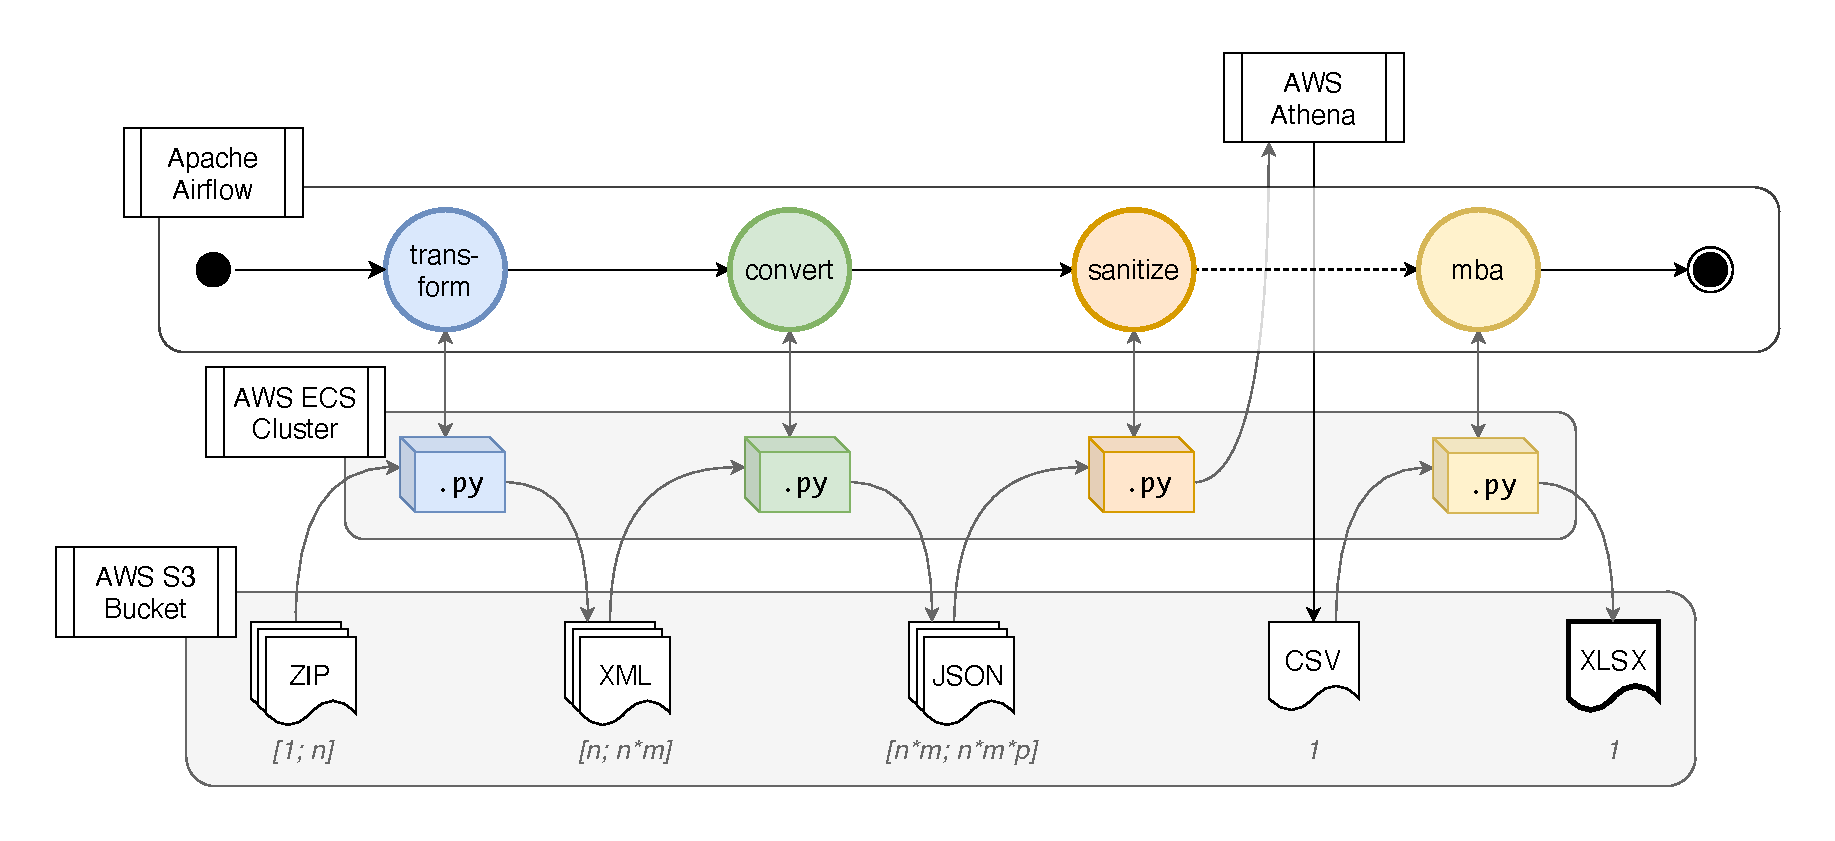
\includegraphics[width=\linewidth]{main-matter/img/5-new-pipeline.pdf}
	\caption{Revisited Data Pipeline Architecture (Server-Less)}
	\label{fig:5-new-pipeline}
\end{figure}

As visualized above, the new architecture outsources the Python analysis scripts out of the Airflow instance. Instead, they create individual microservices now, deployed as virtual containers. These containers, typically realized with the \textit{Docker} containerization software \cite{docker}, contain all required dependencies to run their services. \ac{aws}' \textit{\ac{ecs}} can be used for the server-less deployment and execution of these container tasks \cite{ecs}. With this architecture change, Airflow only remains an orchestration tool that starts the appropriate container tasks. Now, the analytical process is no longer depending on a single virtual server instance. The tasks report their statuses back to Airflow, resulting in Airflow either triggering the next service or terminating the process if an error occurs.

\subsection{Microservice Containerization}
In microservice virtualization, containers are the final desired product. The goal is to have a sequence of commands that encapsulate the Python program code of each individual stage inside their own containers, considering individual stage requirements. To achieve this goal, the intermediate creation of a so-called \textit{image} is required, which provides basic components for making the service runnable \cite{docker}. Before running the container, specific configurations based on the image can been performed.

Docker images are defined by means of a \textit{Dockerfile} \cite{docker}. The tasks inside this file are sequentially executed when creating the image. Exemplarily, the Dockerfile of the Conversion Stage can be seen below.
\newpage
\begin{listing}
	\inputminted{dockerfile}{main-matter/src/5-convert-dockerfile}
	\caption{Dockerfile of the Conversion Stage}
	\label{src:5-convert-dockerfile}
\end{listing}

As can be seen in Source Code Excerpt \ref{src:5-convert-dockerfile}, the image definition begins with referencing the base image (l. 1). This contains a lightweight operating system with the capability of running Python. The Dockerfile also specifies the working directory (l. 2) and prepares environment variables (ll. 4--11) for the container that contain \ac{aws} credentials as well as designated \ac{s3} path \acp{uri} for input and output data locations. The credentials are required for the service to perform its steps on the designated \ac{aws} infrastructure. These environment variables will receive their values during the build process of the container (i.e., when executing the image). This is because such data locations are not expected to remain static for a long period of time. Plus, different data locations have to be provided during the upcoming testing of the containers than during production-grade performance. This data parametrization aids this process. Finally, the local package directory is added to the working directory of the image (l. 16) and all required Python dependencies (for both running and testing) are installed via the \acs{pip} Python package manager (ll. 18--19). These dependencies are specified in the corresponding \texttt{requirements.txt} files inside the package directory.

The environment variables will prove valuable during DataOps enablement. By defining granular \ac{aws} credentials, each stage is only authorized to read and write to their designated \ac{s3} data lake subareas. This creates separated environments for each development stage.

The image can now be build using the \texttt{docker build} command. The design of the Dockerfile requires that the environment variables are passed before container execution (i.e., via arguments in the \texttt{docker build} or \texttt{docker run} command). The image receives a unique tag and the Dockerfile is referenced for correct handling of relative paths. Finally, the image can be used for running the container. This is achieved using the \texttt{docker run} command, specifying which command to run inside the container (e.g., for the Conversion Stage, \texttt{python ./convert.py} for executing the analytics script). This runs the container inside the local system.

\subsection{Image Deployment}
Instead of the container running locally, it is desired to execute it inside the server-less \ac{ecs}. This requires the preliminary deployment to an associated \ac{aws} service, the \textit{\ac{ecr}}. \ac{ecr} is an image repository that is designed to hold different versions of an image \cite{ecr}. This means that each of the four analytics pipeline stages receives its own \ac{ecr}. The image deployment and container execution strategy is depicted in Figure \ref{fig:5-container-deployment} below.

\begin{figure}[h!]
	\centering
	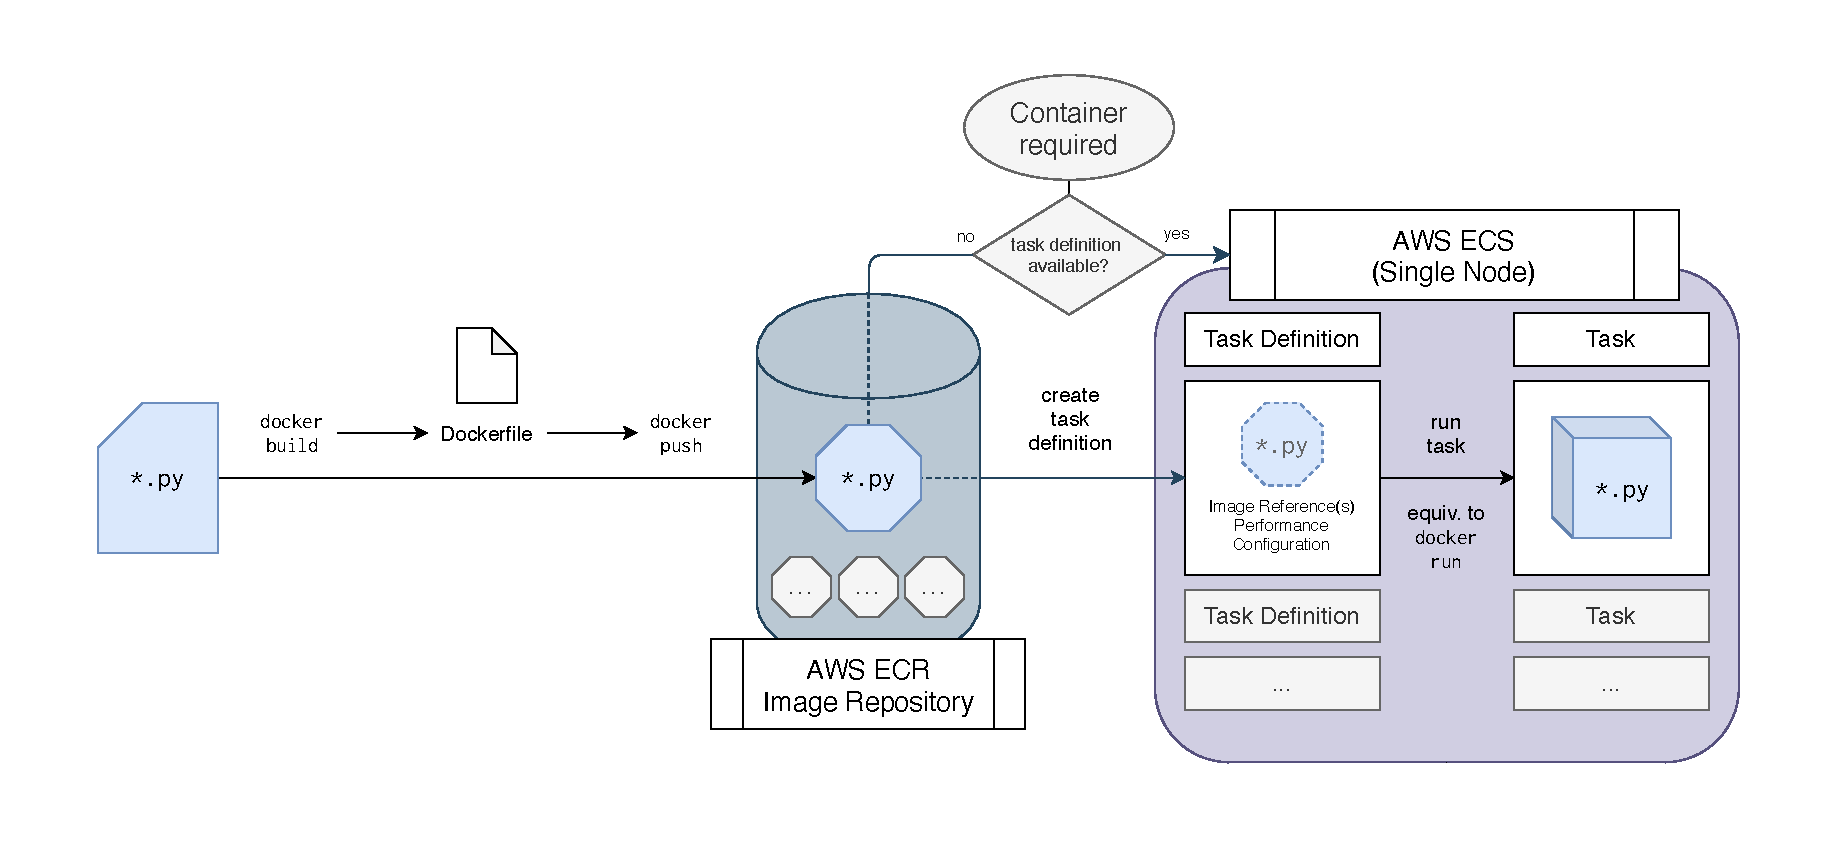
\includegraphics[width=\linewidth]{main-matter/img/5-container-deployment.pdf}
	\caption{Microservice Deployment Process}
	\label{fig:5-container-deployment}	
\end{figure}

Following the flow of the figure, the image is build by means of its Dockerfile and pushed to the designated \ac{ecr}. The octagon shape is used to describe an image. The execution requires another preliminary step which is the task definition of the container. This is because \ac{ecs} can also perform container execution sequences, periodic repetitions of the task, etc. Plus, each task can have different performance requirements. The task definition allows for individual hardware specification (e.g., processing power, memory, etc.) \cite{ecs}. Thus, the task definition can be seen as a blueprint for the (more or less complex) container service. For the data pipeline stages, a task with basic performance specifications as well as one image reference for running the applicable container once, suffices. The task can now be run based on its task definition, providing information on which Python script to run. This executes the task and tears down the container after the task has been worked through or an error has occurred. When the container service is required again and the image repository has not changed, the previous task definition can be directly executed.

\subsection{Server-Less Container Execution via Airflow}
Returning to the high-level overview, creating and running the task definition is performed by Airflow via \texttt{boto3}. The Airflow \ac{dag} controller is redesigned to constantly evaluate the state of \ac{ecr} and \ac{ecs}. It checks for images inside each stage's image repository and builds the applicable task definitions. When all task definitions of all four pipeline stages are present, the Airflow \ac{dag} is ready for execution. The only task inside each individual step of the \ac{dag} is to execute the task definition and evaluate the container response. The \ac{dag} is then executed periodically, e.g. once per day.

Because of the periodic review, the most recent \ac{ecr} images and \ac{ecs} task definition references need to be saved inside Airflow variables to prevent the system from constantly recreating the same task definitions, resulting in an endless loop and, thus, in infrastructure overload.

In case a new version for a stage is recognized, a new task definition is created and re-referenced inside the \ac{dag}, enabling automatic updating of the pipeline solution.

\section{DataOps Enablement}
The next step is to include DataOps-related technologies to the project. They have mostly to do with general solution automation and environment management. Specifically, the following aspects are implemented and configured:

\begin{enumerate}
	\item Enhanced permission management via \acs{aws} \acf{iam},
	\item \acf{vcs} by using \textit{Git} and a \textit{GitHub} repository,
	\item \acf{cicd} by using the \textit{Jenkins} automation software, and
	\item \acf{iac} by using the \textit{Terraform} infrastructure automation tool as well as the \textit{Ansible} infrastructure provisioning software.
\end{enumerate}

These processes will support and build on each other during development for both automation and environment management disciplines.

\subsection{Enhanced Permission Management: \acs{aws} \acs{iam} Roles}
\acs{aws} \acs{iam} roles are used to provide different access permissions to different users and resources. If a user or resource tries to perform actions on \ac{aws} services (e.g., via \acs{cli} or \acs{api}), the system checks if the required credentials are present to perform this action. The credentials are provided in the form of asynchronous encryption, resulting in a public \textit{Access Key ID} and in a private \textit{Secret Access Key} \cite{iam}.

Because of the static nature of the current solution, only one full-access \ac{iam} role is used. This is not desirable from multiple perspectives. Each developer should be provided an \ac{iam} role that is sufficient for his or her needs. The underlying permissions should not exceed these needs in order to prevent collision or changes within \ac{aws} resources outside of the scope of the developer. The same aspect applies to resources that automatically perform actions on other resources. Another important factor is data privacy. In a production-grade environment with sensitive data, it is crucial and binding by law that the data is only seen and processed by authorized entities. 

For instance, if a data pipeline stage is misconfigured and tries to read from another area of the \ac{s3} data lake, the process will terminate when the given \ac{iam} role prohibits this action. Otherwise, the stage would be granted access to data that is not required for its task. In that case, correctly configured \ac{iam} roles can also prevent errors in case the content of the incorrect \ac{s3} area cannot be processed by the current analytics stage.

Considering the \ac{mba} data pipeline, the present variety of resources requires different permissions on a number of other different resources. Table \ref{tab:5-iam} describes all permissions required by different components.

\begin{table}[h!]
	\centering
	\begin{tabular}{r!{\vrule width 1pt}l|l|l}
\textbf{Component}                                  & \textbf{Resource}         & \textbf{Type} & \textbf{Scope}              \\ \ChangeRT{1pt}
\multirow{2}{*}{Airflow}                            & \ac{ecr} & Full Access   & designated stage image repositories          \\ \cline{2-4}
                                                    & \ac{ecs} & Full Access   & designated container service                 \\	 \ChangeRT{1pt}
\multicolumn{4}{c}{\textbf{Stages}}                                                                                           \\ \ChangeRT{1pt}
\multirow{2}{*}{\textbf{Transformation}}            & \ac{s3}  & Read          & \texttt{./landing/}      				  \\ \cline{2-4}
                                                    & \ac{s3}  & Write         & \texttt{./**/raw/}       				  \\ \hline
\multirow{2}{*}{\textbf{Conversion}}                & \ac{s3}  & Read          & \texttt{./**/raw/}       			  	  \\ \cline{2-4}
                                                    & \ac{s3}  & Write         & \texttt{./**/converted/} 				  \\ \hline
\multirow{3}{*}{\textbf{Sanitization}}              & Athena   & Full Access   & designated database                          \\ \cline{2-4}
                                                    & \ac{s3}  & Read          & \texttt{./**/converted/} 				  \\ \cline{2-4}
                                                    & \ac{s3}  & Write         & \texttt{./**/sanitized/} 				  \\ \hline
\multirow{2}{*}{\textbf{\ac{mba}}} 					& \ac{s3}  & Read          & \texttt{./**/sanitized/}  				  \\ \cline{2-4}
                                                    & \ac{s3}  & Write         & \texttt{./**/}          
\end{tabular}
	\caption{\acs{aws} \acs{iam} Role Overview}
	\label{tab:5-iam}
\end{table}

Each data lake scope begins with \texttt{s3://datalake}, specifying the same \ac{s3} bucket for every component. This information is omitted in Table \ref{tab:5-iam} for simplicity reasons. The \texttt{**} symbols represent a wildcard that allow for accessing the different job areas of the data lake. These roles are setup within the \ac{aws} \ac{iam} Console and passed to the individual components as environment variables \cite{iam}, depending on their individual deployment. 

\subsection{\acs{vcs} Enablement: \textit{Git} and \textit{GitHub}}
Embedding the project inside a \ac{vcs} allows for collaborative development. When working with such a system, the common codebase is located inside a distributed repository. This repository can be cloned (i.e., copied) to the developers local development environment. \textit{Committing} to feature \textit{branches} (i.e., performing and saving changes of the personal version of ones source code) does not collide with the source code versions of other developers \cite[9\psqq]{Chacon2020}. Plus, since the project at hand relies on external programming and developing dependencies (e.g., Python packages and libraries, environment configuration processes, etc.), the repository can also contain configuration utilities for setting up the development sandbox.

\subsubsection{Repository Structure}
A cloned repository is a typical project directory. The repository for the \ac{mba} data pipeline solution looks as follows:
\newpage
\begin{figure}[h!]
	\centering
	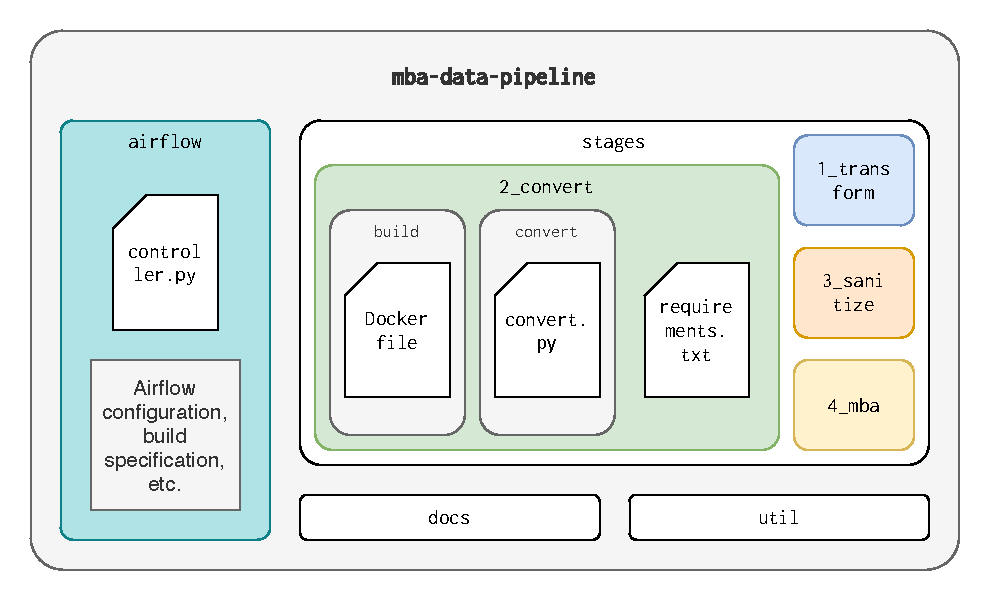
\includegraphics[width=\linewidth]{main-matter/img/5-repo-structure.pdf}
	\caption{Initial Project Repository Structure}
	\label{fig:5-repo-structure}
\end{figure}

The repository presented in Figure \ref{fig:5-repo-structure} is a so-called \textit{monolithic} repository. Since the project is expected to be developed by separate stage teams, this repository de facto consists of multiple projects. Starting at the root of the directory, the repository contains subdirectories for Airflow pipeline management, the individual stages of the data pipeline, documentation as well as miscellaneous utilities. The Airflow pipeline management consists of the pipeline controller script, as well as supporting build files that are outside the scope of this thesis. More importantly, the individual stages are, again, divided into subdirectories. Each stage has its own build directory (currently including its Dockerfile), a package directory (currently including all productive source code), as well as dedicated requirements files required by the source code.

\subsubsection{Repository Setup}
The goal is to create a GitHub repository for the \ac{mba} data pipeline project. First, the project needs to become a Git repository, enabling the version control capability. GitHub is used for the distribution and collaborative management of the code base \cite[25\psqq]{Chacon2020}\cite{github}. First, the project directory needs to be initialized by means of Git. Then, the repository can be created within the GitHub web \ac{ui}. Lastly, the local Git repository is pushed to the recently created GitHub repository.

In order to allow for the automatic configuration of development sandboxes, each stage directory receives a \textit{Makefile} that creates shortcuts for configuration commands. This includes local building and executing of a Docker container. Other development conventions (e.g., for Python, that development should be conducted in Python \textit{virtual environments}), cannot be enforced but only suggested within the project documentation.

\subsubsection{Branching Strategy}
Currently, an authorized developer is able to clone this repository, make any kind of changes, and push these changes back to the repository. This kind of workflow is not desired which is why \textit{branching} is introduced. Branching is a GitHub feature that supports development environment management within the repository \cite[62\psqq]{Chacon2020}. At this point, only one branch, the \texttt{master} branch, exists. It holds the history of all versions of the source code. These versions change when updated code is pushed to the brach. In practice, the \texttt{master} branch is supposed to be the communal \textit{single version of the truth}. It is expected to be runnable and should reflect the source code of the solution which is currently used in production. When changes of all sorts are possible inside the \texttt{master} branch, the validity of it gets lost. This is why this branch needs to be protected such that only evaluated changes can be pushed to this area of the repository.

Branching is a matter of project convention definition. The general goal is that on-going development of an arbitrary feature is conducted outside of the \texttt{master} branch (i.e., on separated feature branches). Each (sub-)team working on an individual feature \textit{branches} from the \texttt{master} branch, resulting in an exact copy of its origin in the beginning. All changes pushed to the new branch do not affect the \textit{master} brach. When the feature is considered done, a GitHub \textit{pull request} is created \cite{github}. This pull request is evaluated based on its configuration. If the evaluation passes, the feature branch gets \textit{merged} with the \texttt{master} branch, meaning that all changes are applied to the source code inside the \texttt{master} branch at once. Finally, the feature branch is deleted. From now on, the updated \texttt{master} branch is used as the starting point for further development. This branching workflow is commonly referred to as the \textit{GitHub Flow} \cite{GitHub2020}, depicted in Figure \ref{fig:5-github-flow}.
\newpage
\begin{figure}[h!]
	\centering
	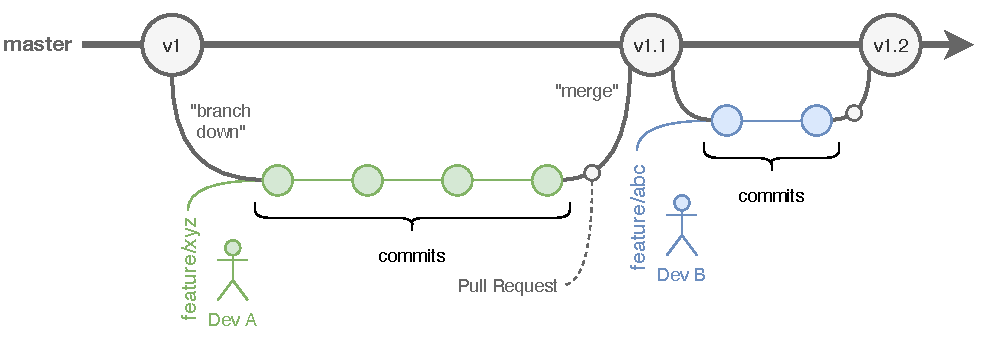
\includegraphics[width=\linewidth]{main-matter/img/5-github-flow.pdf}
	\caption[\textit{GitHub Flow} Branching Strategy]{\textit{GitHub Flow} Branching Strategy (per \cite{GitHub2020})}
	\label{fig:5-github-flow}
\end{figure}

The branching strategy, as presented above, is typical for a fast-paced development cycle. Each approved change, no matter how small, is directly published into production. Apart from that, other branching strategies could be applied. It might be reasonable to include separate \texttt{development} and \texttt{release} branches. The \texttt{development} branch could become the starting point for new features and could contain features that have not been published yet. In case of a slower release cycle, the development branch could be merged with the \textit{release} branch for compatibility testing purposes and deployed into production (i.e., merged with the \texttt{master} branch) afterwards. Another \texttt{hotfix} branch might be used for quick bug fixes that branches from the \textit{master} branch, fixes the bug, and merges back into production \cite{Driessen2010}.

For the sake of simplicity and demonstrability, the former described branching strategy is chosen for the \ac{mba} data pipeline. The \texttt{master} branch is configured inside GitHub to only accept pull requests for incoming changes, not direct pushed onto the \texttt{master} branch. Later, the pull request functionality will be enriched with \ac{cicd}. In case the process runs through without errors, the changes are evaluated positively and cleared for the merging process.

\subsection{\acs{cicd} Enablement: \textit{Jenkins}}
\ac{cicd} is expected to enhance and automate two aspects inside the development process of the \ac{mba} data pipeline solution:
\begin{enumerate}
	\item It handles the build and deployment of virtual Docker images and containers by means of Figure \ref{fig:5-container-deployment}. This also includes providing each task with its designated environment variables for infrastructure access as well as analytics data input and output locations.
	\item It automates the execution and reporting of test cases, only allowing for approved deployment of tested versions of the solution. This process supports the previously mentioned pull requests which will fail when tests are evaluated negatively.
\end{enumerate}

The latter aspect will be implemented in Section \ref{sec:5-testing-implementation}.

The desired DataOps \ac{cicd} workflow is depicted in Figure \ref{fig:5-cicd}. It considers testing a black box for now. It is noteworthy to mention that each stage of the data pipeline could have different requirements for its deployment, which is why each stage receives its own \ac{cicd} pipeline. This becomes clear when considering testing since each stage performs different tasks and requires different test cases.

\begin{figure}[h!]
	\centering
	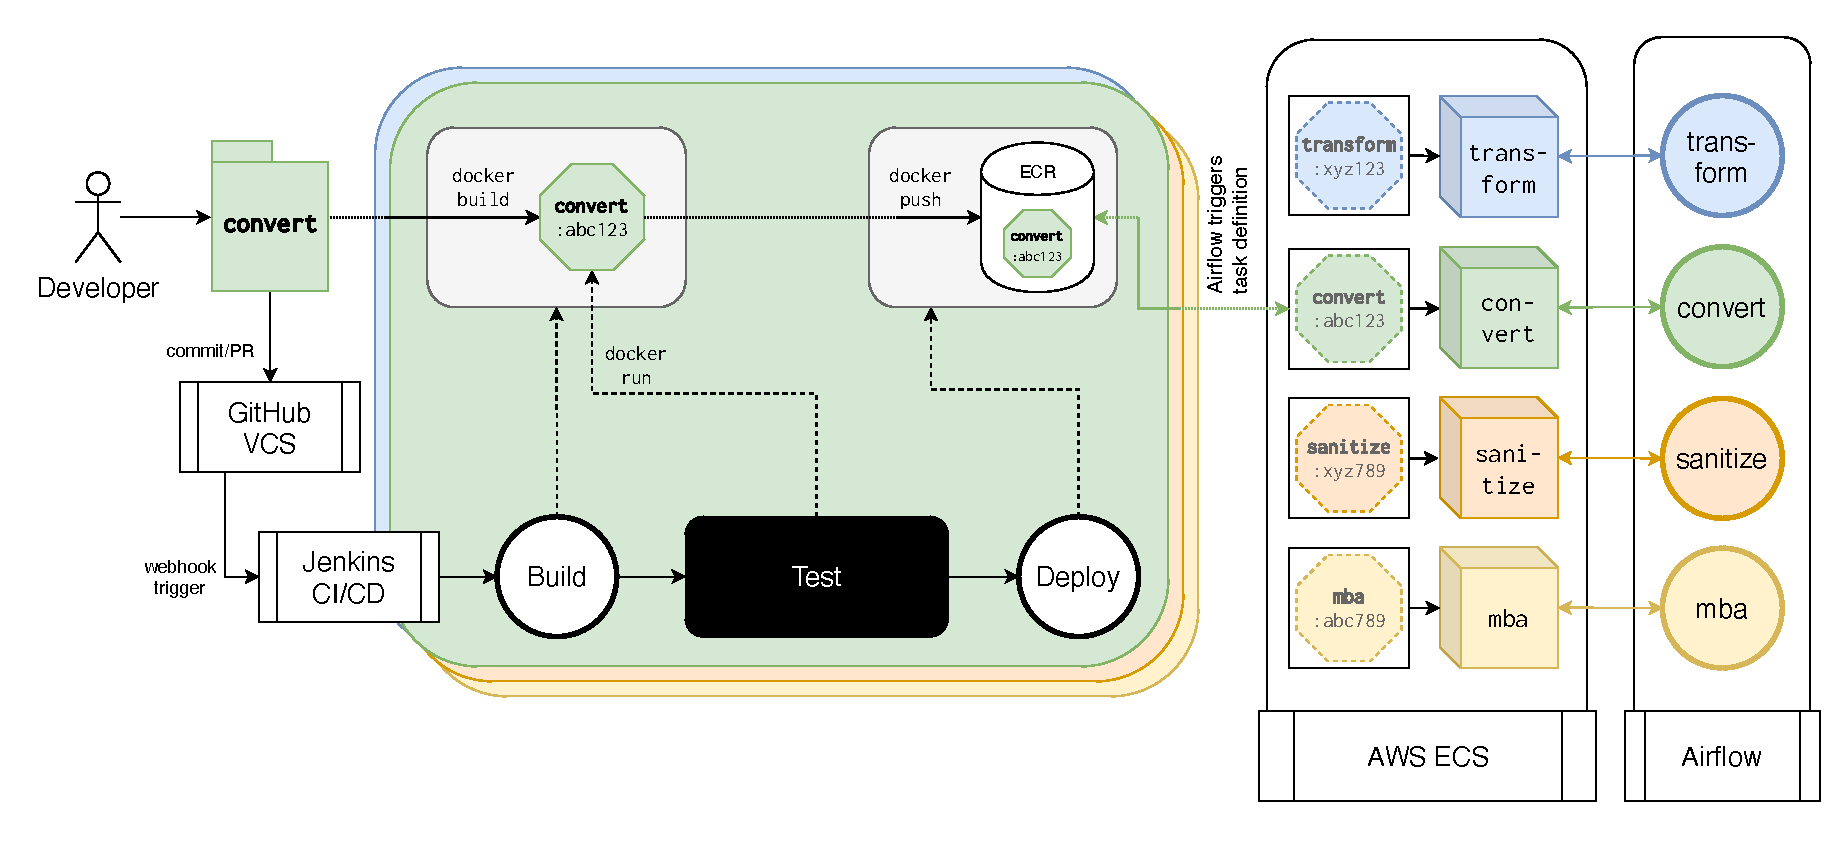
\includegraphics[width=\linewidth]{main-matter/img/5-cicd.pdf}
	\caption{DataOps \acs{cicd} Architecture for the Conversion Stage}
	\label{fig:5-cicd}
\end{figure}

Figure \ref{fig:5-cicd} represents the \ac{cicd} workflow of the Conversion Stage. It is meant to be executed whenever a GitHub pull request of a Conversion Stage-related feature is opened. This pull request appearance should trigger the corresponding pipeline, realized with the \textit{Jenkins} \ac{cicd} software \cite{jenkins}. The first step needs to build a virtual Docker image using the target source code files from the pull request. Again, this build process is done by means of the stage's specific Dockerfile and requires additional arguments for the containers environment variables. When the image is built, the build stage of the \ac{cicd} pipeline is completed. Later, this this image will be run on the Jenkins instance for different testing purposes. After these tests pass, the image is ready for deployment. Airflow expects runnable images inside their designated \ac{ecr} repositories which is why the image, individually tagged, is pushed to its repository. The deployment process is done at this point. When Airflow needs to run a new analysis, the controller script will scan the registry for the latest image, recognize a new image, create the applicable task definition and run the container based on the newly deployed image. Every further analysis will be done utilizing this image until a new image is deployed again.

\subsubsection{Jenkins Software and Pipeline Setup}
Comparable to Apache Airflow, Jenkins needs to be considered as an external application that needs to reside on some kind of infrastructure. For efficiency reasons, the \ac{ec2} instance already running Airflow also receives Jenkins. Both web servers now run simultaneously on different ports for \acs{http} access.

Jenkins provides different blueprints for \ac{cicd} pipelines. The DataOps \ac{cicd} pipeline of the \ac{mba} data pipeline needs to recognize pull requests that originate from different feature branches within GitHub. This is why the \textit{Multibranch Pipeline} is chosen \cite{jenkins}. Such a pipeline is created for each of the four stages of the data pipeline. The branch needs to be granted access to the GitHub repository. Since the project is working with a monolithic repository, each \ac{cicd} pipeline needs to be configured in such a way that it only recognized changes and pull requests to specific areas of the repository.

There are multiple ways to achieve this configuration. Jenkins distinguished between branches and pull requests, meaning that a branch with a pending pull request is listed and evaluated by Jenkins \textit{twice}. Jenkins is therefore configured to disregard branches that are also filed as pull requests. The only non-pull request branch should be the \texttt{master} brach since all other branches are expected to be in development if no pull request is present. Thus, Jenkins should only consider \texttt{master} a long-lasting branch. The pipeline should only consider stage-specific changes, which is why Jenkins should filter each pull request by its GitHub label. This requires the developer to add the specific stage label when filing a pull request. Finally, Jenkins should automatically run a \ac{cicd} job inside the corresponding pipeline when a change is recognized. This needs to be enabled in both Jenkins and GitHub. GitHub needs to send a \texttt{POST} request to Jenkins when a pull request is filed, whereas Jenkins needs to trigger the corresponding pipeline on \texttt{POST} request arrival.

\subsubsection{Jenkins Credential Management}
The virtual microservices need to receive their \ac{aws} \ac{iam} access credentials during their build process. Since this process is expected to be covered by \ac{cicd}, Jenkins needs to hold these credentials and pass these to the corresponding stage containers inside its \ac{cicd} pipeline workflow. This is achieved by adding the individual credentials to Jenkins' encrypted credential storage \cite{jenkins}. These need to include all stage-related credential key-value pairs that provide appropriate access to the analytics resources as described in Table \ref{tab:5-iam}. Additionally, Jenkins needs to be granted permission to push images to the \ac{ecr} repositories. The corresponding credential should not be mistaken with a separate \ac{iam} role. Rather, Jenkins needs to hold a login token for \ac{ecr} that is retrieved via \ac{aws} \acs{cli} \cite{ecr}. This process is identical to other Docker registry services, independent from the actual vendor.

Jenkins will then pass the encrypted credentials to the corresponding pipelines \cite{ecr}, resulting in no hard-coded credentials in any configuration file.

\subsubsection{Pipeline Workflow Declaration}
After the pipeline preferences have been configured, the actual pipeline workflow needs to be declared for each stage. In Jenkins, this is done via a so-called \textit{Jenkinsfile}. It is written in \textit{Groovy} programming language and contains instructions for each stage of the pipeline \cite{jenkins}. A sample Jenkinsfile for the Conversion Stage is shown below.

\begin{listing}[h!]
	\inputminted{groovy}{main-matter/src/5-jenkinsfile-build}
	\caption{Jenkinsfile Build Stage for the Conversion Stage}
	\label{src:5-jenkinsfile-build}
\end{listing}

Source Code Excerpt \ref{src:5-jenkinsfile-build} shows the build stage inside the Jenkinsfile. It retrieves the corresponding stage credentials from Jenkins' credential storage (ll. 8--11) and executes the build process of the Docker image (ll. 12--19). The image needs to be tagged in an \ac{aws}-provided \ac{ecr} format such that it is assigned to the correct repository during the deployment phase. This tag includes the corresponding Git commit ID for versioning purposes (l. 14) which is passed to Jenkins by the previously mentioned GitHub \texttt{POST} request trigger. Prior to the build, the arguments for the \ac{aws} \ac{iam} credential pair are passed (ll. 15--16) and set as environment variables by means of the Dockerfile specification. Later, the remaining arguments for input and output data locations will be covered by Airflow when calling for a new analytics job. Finally, the Dockerfile (l. 17) and the build context for relative path recognition (l. 18) are specified. This command is executed by the Jenkins \ac{cicd} pipeline job. In case of a correct execution, the next stage is performed. Since testing is omitted for now, it directly continues with the deployment, shown below. 

\begin{listing}[h!]
	\inputminted{groovy}{main-matter/src/5-jenkinsfile-deploy}
	\caption{Jenkinsfile Deployment Stage for the Conversion Stage}
	\label{src:5-jenkinsfile-deploy}
\end{listing}

Source Code Excerpt \ref{src:5-jenkinsfile-deploy} shows the deployment stage inside the Jenkinsfile. It retrieves the \ac{ecr} credentials (ll. 11--13) and performs the image deployment via \texttt{docker push} (ll. 14--17). This action is performed for two tags: the commit ID for versioning and the conventional \texttt{latest} tag such that Airflow recognizes it as the most recent, production-ready image. \\\

All in all, the current \ac{cicd} solution builds and deploys a new version into production when a feature pull request is filed to GitHub. Airflow recognizes the change based on its controller script and uses the new image for the corresponding stage for container execution and evaluation.

\subsection{\acs{iac} Enablement: \textit{Terraform} and \textit{Ansible}}
Another form of automation that is part of DataOps is automatic infrastructure deployment via \ac{iac}. The project at hand requires a variety of different \ac{aws} infrastructural resources, including the effort of configuration. In case that the infrastructure needs to be setup inside a different \ac{aws} account or it breaks during development, it is not desirable to be forced to start building up the infrastructure from scratch. Instead, the following \ac{iac} architecture is proposed.

\begin{figure}[h!]
	\centering
	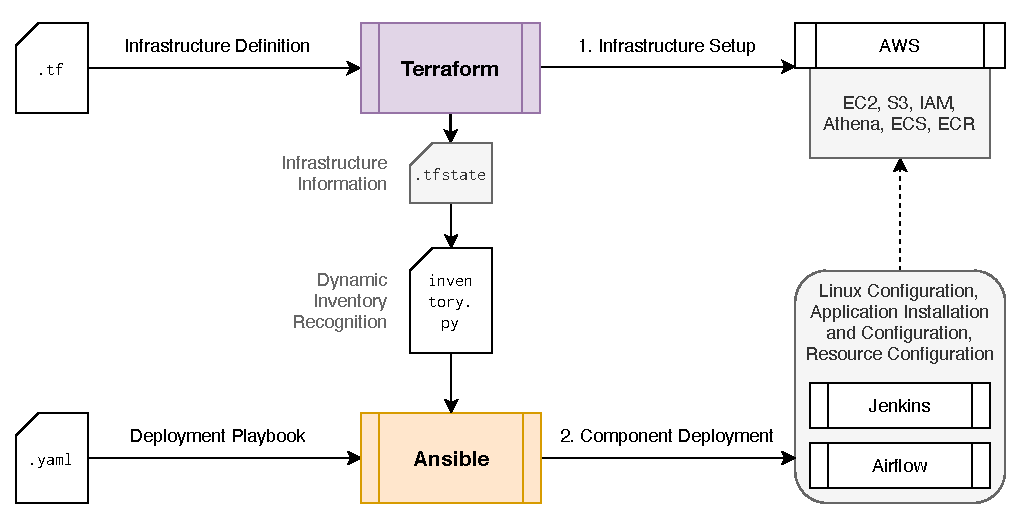
\includegraphics[width=\linewidth]{main-matter/img/5-iac}
	\caption{\acs{iac} Infrastructure Deployment Strategy}
	\label{fig:5-iac}
\end{figure}

The \ac{iac} architecture, visualized in Figure \ref{fig:5-iac}, is made out of two steps. First, all required \ac{aws} services are defined for the \textit{Terraform} infrastructure provisioning tool. This also includes basic configuration of networking and access management. In general, all configuration that can be done via the web \acs{ui}-based \ac{aws} Console or the \ac{aws} \acs{cli} or \acs{api} can be done via Terraform. Terraform requires an individual \ac{iam} role that allows it to create the infrastructure. When the deployment script is performed via the Terraform \acs{cli}, it creates a \texttt{.tfstate} file in \ac{json} format \cite{terraform}, summarizing all created infrastructure including public IP addresses, infrastructure IDs, etc.

This infrastructure needs to be configured via the \textit{Ansible} infrastructure orchestration software. This includes the Linux configuration of the \ac{ec2} instance, the creation of \ac{s3} data lake (sub-)areas, etc. Basically, the goal is to run the corresponding commands for Terraform and Ansible, resulting in an up-and-running infrastructure, ready for production-grade usage.

Ansible requires an intermediate step before being able to perform actions on the infrastructure, which is the recognition of the resource inventory. This can be done manually, which is not desired, or via a dynamic inventory recognition script. This makes use of the previously generated \texttt{.tfstate} file and provides Ansible with information and access to the respective infrastructure. Then, so-called Ansible \textit{Playbooks} are written and executed. These hold tasks for the configuration, platform and application installation, etc. \cite{ansible}. Most importantly, Ansible is in charge of installing and configuring Airflow and Jenkins. Airflow is installed and receives its controller script as well as further configuration from the project repository. Jenkins is installed, pre-configured, and required plugins are installed. 

Unfortunately, these applications do not provide all necessary Ansible endpoints. This means that not all configuration steps can be done automatically but require manual adjustment. This includes Jenkins credential management, pipeline creation, etc. All in all, the infrastructure automation is valuable nonetheless since the manual setup process is significantly reduced.

\section{Testing Framework Implementation} \label{sec:5-testing-implementation}
At this point, the DataOps capability of the \ac{mba} pipeline solution is sufficient to be enhanced by means of the testing framework, designed in Chapter \ref{chap:testing-framework}. The practical implementation of the framework goes hand-in-hand with its design steps.
\begin{enumerate}
	\item The data event handling mechanisms need to be implemented inside the productive analytics solution.
	\item The test data (suites) need to be provisioned inside a separated data environment.
	\item DataOps solution tests need to be written and executed by the Jenkins pipeline, making use of the available test data. The test outcome evaluation inside Jenkins will decide if the given version update may be deployed into production.
\end{enumerate}

\subsection{Data Event Handling Implementation}
In general, the goal is that the data event handling inside the solution complies with its corresponding definition. When summarizing all event handling processes by means of their actions, the following capabilities need to be ensured:

\begin{itemize}
	\item Logging of different event severities.
	\item Process termination for \texttt{CRITICAL} events.
	\item Threshold adjustment and evaluation for \texttt{ERROR} and \texttt{WARNING} events.
	\item Dynamic File Flagging for \texttt{ERROR} and \texttt{WARNING} events.
\end{itemize}

Again, there are multiple ways to achieve this kind of data handling capability in practice. In order to keep the productive analytics source code readable and maintainable, data handling is outsourced to its own class \texttt{DataHandling} that is instantiated inside the solution. It receives the references to the data in question, threshold limits, etc. during initialization. Each data event definition receives its own function which is then called by the solution at the appropriate point during its runtime. The visualization of the Conversion Stage, including all its data event handlers, can be found in Appendix Figure \ref{app:new-convert}.

For the sake of clarity, the following paragraphs elaborate on the implementation of the list of general features inside the \texttt{DataHandling} class before presenting exemplary implementations of several data handling functions.

\subsubsection{Event Logging}
Event logging in Python can be realized with Python's standard \texttt{logging} library. The default log severities \texttt{INFO}, \texttt{WARNING}, \texttt{ERROR}, and \texttt{CRITICAL} correspond with the event severities of the testing framework. The \texttt{logging} object is instantiated inside the \texttt{DataHandling} class and configured to write log occurrences of severity \texttt{INFO} and above to a specified file which receives the name of the current analytics job. Each time a log is required, the \texttt{logging} object is called with the message and arguments to be contained.

\subsubsection{Process Termination}
The analytical process needs to be terminated whenever an event of \texttt{CRITICAL} severity occurs. In order to provide helpful monitoring information, the termination should not just shut down the process. Instead, it should prompt a message on why the process needed to be terminated. On the one hand, this is included to the log file by means of the previous section. On the other hand, each critical event receives its own custom Python \textit{Exception}. This exception contains are log-like information message as well as a traceback to the origin of the exception, and hence, termination. This is expected to allow for better understanding and recovery from the underlying issue.

\subsubsection{Thresholding Capability}
As previously mentioned, the threshold percentages are passed to the \texttt{DataHandling} class during initialization. Currently, a value of $0.05$ for \texttt{ERROR} events and $0.1$ for \texttt{WARNING} events, is utilized. This means that five percent of the input data may invoke \texttt{ERROR}s and ten percent of the data may invoke \texttt{WARNING}s. The solution does not take files with multiple data issues into account differently. Eventually, the most severe event is counted for threshold evaluation. At the end of the input data event handling process, the threshold values are evaluated. The process terminates when either one of the thresholds is exceeded. As previously described, transformation and output data is not subject to threshold evaluation but results in instant termination in case an event is invoked (cf. Section \ref{sec:4-1-4}).

\subsubsection{File Flagging}
\texttt{WARNING} and \texttt{ERROR} events additionally flag files by means of their invocation event. The \ac{aws} Python \ac{sdk} \texttt{boto3} is used for this matter since all data resides inside the \ac{s3} data lake. File flagging is implemented inside its own function which is called with the appropriate file reference (i.e., the file to be tagged) and the tag itself. \texttt{boto3} then requests all current tags for the file. In case the tag in question has not been set, it is added to the file now. The tagging information is provided inside the log file with \texttt{INFO} log severity.
\newpage
\subsubsection{Event Handling Implementation Examples}
Now that the components of the event handing are defined, the individual handling functions can be implemented. The following examples go by the data event examples provided in Section \ref{sec:4-1-3-a}, \ref{sec:4-1-3-b}, and \ref{sec:4-1-3-c}.

\paragraph{Example A: Data Source Empty}
\begin{listing}[h!]
	\inputminted{python}{main-matter/src/5-a.py}
	\caption{Implementation of Data Event Example A: Data Source Empty}
	\label{src:5-example-a-implementation}
\end{listing}
Source Code Excerpt \ref{src:5-example-a-implementation} implements the data event handling for an empty data source. The function receives the file references as a parameter (l. 1) and makes use of a \textit{guard} statement to rule out an empty data source first (l. 2). In case this condition does not apply, the function logs the \texttt{CRITICAL} event to the log file, providing information on the \ac{s3} bucket and bucket directory in question (ll. 4--8). These have been passed to the class instance during initialization. At the end, it raises the custom \texttt{S3EmptyError} exception that terminates the process. The exception is prompted, again, with bucket and directory information (l. 9) for improved troubleshooting.
\newpage
\paragraph{Example B: XML File(s) Corrupted}
\begin{listing}[h!]
	\inputminted{python}{main-matter/src/5-b.py}
	\caption{Implementation of Data Event Example B: \acs{xml} File(s) Corrupted}
	\label{src:5-example-b-implementation}
\end{listing}
Source Code Excerpt \ref{src:5-example-b-implementation} implements the data event handling for corrupted \ac{xml} files. Again, the corresponding function receives file references. Since there is a possibility that other \texttt{ERROR} events have already occurred and removed faulty input data, the function checks if there are any files left for evaluation (l. 2). Then, it loops through all files in question and attempts to parse their binary content to \ac{xml} (ll. 6--7). The function makes use of the Python \ac{xml} \texttt{ElementTree} sub-library (initialized as \texttt{et}). By design, the parser function raises an \texttt{ParseError} exception if the data is corrupted. By catching this library exception, the specific data handling can be processed. The log file receives a new line containing the corresponding file information (ll. 9-11). Additionally, the log also mentions that the file in question is skipped because of the \texttt{ERROR} event severity. The file name reference is added to another list that contains all corrupted files (l. 4 and 13) and the error file counter is incremented (l. 14). This will later be used for threshold evaluation. Finally, all corrupted files are removed from the original file reference dictionary (l. 15--16).
\newpage
\paragraph{Example C: Missing Optional Attributes}
\begin{listing}[h!]
	\inputminted{python}{main-matter/src/5-c.py}
	\caption{Implementation of Data Event Example C: XML File(s) Corrupted}
	\label{src:5-example-c-implementation}
\end{listing}
Source Code Excerpt \ref{src:5-example-c-implementation} implements the overall data event handling for missing global attributes. Since the event in question only covers the missing \textit{optional} attributes, the handling of required attributes is omitted here (l. 6). At this point of the analysis, the binary \ac{xml} data has already been parsed to Python standard dictionaries, which is why the function received a dictionary of all \ac{pos} dictionaries (l. 1) and loops over the root dictionary (l. 2). As with the first example, a guard statement is used to rule out the case of any missing argument (ll. 3--4). Then, the keys of the content dictionary are evaluated against the constant class list of optional attributes (ll. 8--10). In case this evaluation results in arguments missing, a list of missing attributes is created (ll. 11-13) and logged alongside the input file name (ll. 14--20). Since this is an event of \texttt{WARNING} severity, the \texttt{WARNING} event file counter is incremented (l. 21) and evaluated at the end of input data event handling. Finally, the source data tagged via the custom tagging function (ll. 22-26)

All further data events are implemented in a similar manner.

\subsection{Test Data Provisioning}
In order to test for correct data handling, appropriate test data is required to invoke the corresponding events. The design of the test data suited of various complexity degrees and use cases has been conducted in Section \ref{sec:4-test-data-design}. The goal now is to provision these suites in order for the planned, holistic DataOps testing integration. Specifically, the test data needs to be available for continuous testing in every phase of development. Since a centralized data lake already exists, the goal can be achieved by adding the test data to the data lake.

\subsubsection{Data Lake Architecture Revision}
The current architecture of the data lake only considers production-grade analytics processes. Simply adding the test data inside this critical environment could be prone to compatibility and analytics correctness issues. Plus, it goes against the DataOps principle of distinct environments. This is why the following data lake architecture revision is proposed:

\begin{figure}[h!]
	\centering
	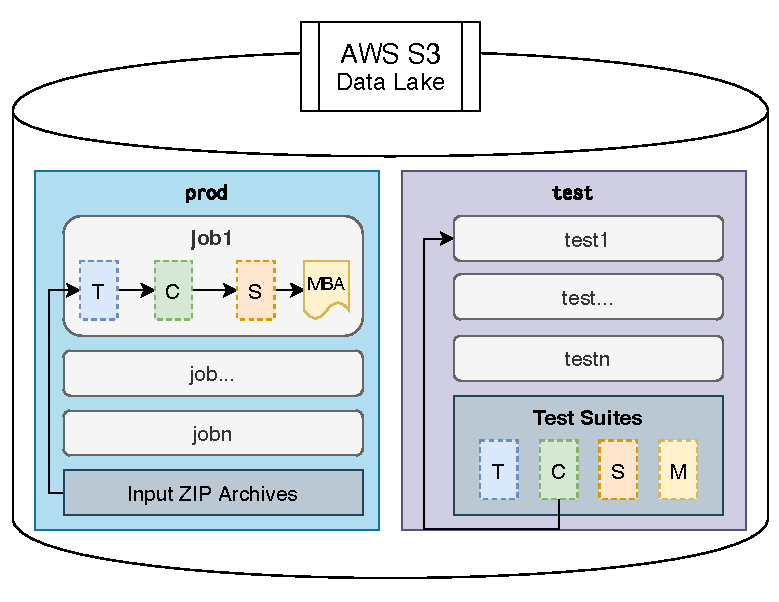
\includegraphics[width=0.67\linewidth]{main-matter/img/5-data-lake-new}
	\caption{Data Lake Architecture Revision}
	\label{fig:5-new-data-lake}
\end{figure}

In the new structure, presented in Figure \ref{fig:5-new-data-lake}, the data lake is environmentally divided at the topmost level. One environment remains the otherwise unchanged production-grade environment, containing raw input data as well as all analytics job subareas. The new testing environment now contains input data test suites for every stage of the pipeline. Since this data is also expected to be processed by the corresponding stage during testing, the area has also got job subareas for each conducted test.
\newpage
With this change, the stages do not conduct test-grade analysis with production-grade data, but remain in a separated testing environment. The corresponding \ac{s3} \acp{uri}, containing test data, are passed to the individual stages. In case all future tests pass, the stages are permitted to receive the production-grade data locations afterwards.

\subsubsection{\acs{iam} Role Revision}
With new environments, new \ac{aws} \ac{iam} roles are required. This maintains another layer of analytical integrity. In case a test stage receives production-grade data references, a correctly configured \ac{iam} role prevents it from performing. Developer sandboxes and their \ac{iam} roles can also be changed here such that the personal environment does not have access to potentially sensitive data.

In practice, each stage receives a second \ac{iam} role for testing purposes. The corresponding credentials are passed as environment variables to the virtual stage container and replaced with the production-grade access credentials after the tests have passed. \\\

With this method of test data provisioning, each environment (i.e., developer sandbox, local or \ac{cicd}-integrated testing, etc.) has access to the test data suites while restricting access to sensitive, production-grade data at the same time.

\subsection{DataOps Testing Implementation}
The DataOps testing implementation is expected to ensure that a new version of a solution is running as expected before being deployed into production. This requires separate testing classes that evaluate the functionality of the solution based on expected outcomes. As described in Section \ref{sec:4-3-testing-architecture}, this includes all testing levels (i.e., unit, integration, and end-to-end testing) covering both software and data-driven aspects of the solution. 

In general, the Python testing framework \textit{PyTest} as well as applicable Python standard testing functions can be utilized for this purpose. With PyTest, individual testing classes are created. Each function inside a testing class can be seen as a single testing use case. The testing process in general performs a number of preparatory measures, runs the code piece at test and evaluates the outcome of the code under test. This happens by means of a comparison to the expected outcome. If these values correlate, the test passes and the next test case is performed. Otherwise, the test case fails and is prompted.

The following paragraphs implement the testing classes for all testing levels of the Conversion Stage.

\subsubsection{Unit Testing Implementation}
The unit tests for the Conversion Stage are expected to cover the granular, software-driven aspects of the solution. Per testing convention, the functionality of external libraries is expected to have already been tested such that these do not require additional testing. Therefore, the extraction of data source and destination locations and \ac{aws} \ac{iam} credentials remain subject to unit testing.

The outsourced \texttt{env} module covers this functionality. It received the corresponding values through a function given by the Python standard library \texttt{os}. There are multiple events that are caught at this point, which should not be mistaken with data events. The current events make sure that the \ac{s3} data location \acp{uri} are provided in the correct format. The remaining functions of the module extract individual parts of the \ac{uri} that are required by the solution at the point where these functions are called. Credential extraction is designed similarly. These functions represent the code under test for Conversion Stage unit testing.

The practical unit tests passes incorrectly formatted \ac{s3} \acp{uri} to the retrieval function and expects it recognize the issue and terminate the process. One of the test cases also provides a well-formatted \ac{uri} and expects that no issue is reported. The component extraction functions (for \ac{s3} bucket name and path extraction) are only invoked when the retrieval function reported no error. Thus, their test cases only pass correct \acp{uri} and compare their outcome (e.g., an \ac{s3} bucket name) to the hard-coded expectation based on the corresponding input \ac{uri}.

\subsubsection{Integration (Data) Testing Implementation} \label{sec:5-3-3-2}
Integration testing of the Conversion Stage evaluates the data handling measurements based on the predefined test data suites residing in the testing environment of the \ac{s3} data lake. Therefore, it plays a major role for Conversion Stage testing because of the large number of data events and the data-driven nature of the stage in general.

Since the stage is expected to be capable of handing events regarding data format, schema, and value, three separate testing classes are created for the integration testing level. Now, each of the data event handling functions needs to be tested holistically. Specifically, the goal is to ensure the following aspects:

\begin{itemize}
	\item The appropriate data event handling function is called at the appropriate point inside the analytics solution.
	\item The data event handling function performance complies with its definition (i.e., it performs all required measures if the event occurs).
\end{itemize}

The tests are supported by the previously defined test data suites, specifically the single-event and multi-event test data files (cf. Sections \ref{sec:4-single-event} and \ref{sec:4-multi-event}) that are now used to evaluate the performance of the data event handling. They are retrieved prior to the test execution and specified for each test case individually.

The following paragraphs present the testing implementation of the data event handling function that checks for corrupted \ac{xml} files. This example provides the most individual test cases for a single data event out of the previously mentioned examples. Since corrupted \ac{xml} files belong to the data format issue category, the tests are included inside the \texttt{TestCovertDataFormat} class. All of the test cases are performed with a single test data file that represents an actually corrupted \ac{xml} file.

\paragraph{Data Handling Function is Called}
\begin{listing}[h!]
	\inputminted{python}{main-matter/src/5-corrupted-calls.py}
	\caption{Data Handling Function Call Test for Corrupted \acs{xml} Files}
	\label{src:5-corrupted-calls}
\end{listing}
Source Code Excerpt \ref{src:5-corrupted-calls} represents the test case function that evaluates if the \texttt{remove\_corrupted(...)} function is called within the \texttt{xml\_to\_dict(...)} function of the analytics solution. Since the function call itself is always required, the input data for the function does not play a role. Since the data handling function is not explicitly known by the test function, it is mocked by the PyTest framework (l. 2). Then, \texttt{xml\_to\_dict(...)} is called with an empty dictionary (which is arbitrary here) (l. 3). Finally, the test \textit{asserts} that the data handling function was indeed called (l. 4). An assertion in general returns \texttt{True} if the given condition (here, the function call) applies. If not, it returns \texttt{False}. 
\newpage
\paragraph{Data Handling Function Skips Corrupted File}
\begin{listing}[h!]
	\inputminted{python}{main-matter/src/5-corrupted-skips.py}
	\caption{Data Handling Function Test for Skipping Corrupted \acs{xml} Files}
	\label{src:5-corrupted-skips}
\end{listing}
Source Code Excerpt \ref{src:5-corrupted-skips} represents the test case function that evaluates if the a corrupted \ac{xml} file is skipped within the \texttt{xml\_to\_dict(...)} function of the analytics solution. The implementation does not explicitly test the data handling function but its actions. This approach was chosen since the implementation of such a function might change, but the fact that corrupted \ac{xml} files cannot be processed does not change. The function specifies the corrupted \ac{xml} file (l. 2) and loads it inside a Python dictionary from the \ac{s3} bucket (ll. 4--8). This dictionary is required by the \texttt{xml\_to\_dict(...)} function as its parameter. The function is then called with the prepared dictionary (l. 11). Since the corrupted file has been the only file in scope of the test, the test finally asserts if the dictionary is empty after the function call which would mean that the file has been skipped successfully. Since this process is also logged, the test function mocks the logging mechanism (l. 10) and asserts that the information has been added to the log file (l. 13). 
\newpage
\paragraph{Data Handling Function Logs Corrupted File}
\begin{listing}[h!]
	\inputminted{python}{main-matter/src/5-corrupted-logs.py}
	\caption{Data Handling Function Test for Logging Corrupted \acs{xml} Files}
	\label{src:5-corrupted-logs}
\end{listing}
Source Code Excerpt \ref{src:5-corrupted-logs} represents the test case function that evaluates if a corrupted \ac{xml} file is logged when the \texttt{xml\_to\_dict(...)} function is executed. The process is very similar to the example above. The data is retrieved from \ac{s3} (ll. 4--8), the logging mechanism for \texttt{ERROR} logs is mocked by PyTest (l. 10), and the \texttt{xml\_to\_dict(...)} function is called with the resulting dictionary (l. 11). The assertion evaluates the predefined string for corrupted \ac{xml} files matches with the actual outcome of the function call.

\paragraph{Data Handling Function Tags Corrupted File}
\begin{listing}[h!]
	\inputminted{python}{main-matter/src/5-corrupted-tags.py}
	\caption{Data Handling Function Test for Tagging Corrupted \acs{xml} Files}
	\label{src:5-corrupted-tags}
\end{listing}
Source Code Excerpt \ref{src:5-corrupted-tags} represents the test case function that evaluates if a corrupted \ac{xml} file is tagged inside the \ac{s3} bucket when the \texttt{xml\_to\_dict(...)} function is executed. Again, the preliminary steps (ll. 3--11) are identical to the previous test cases. Only a \texttt{boto3} \textit{Client} (l. 2) for an \ac{s3} tag request (ll. 12--14) is added. This request returns a list of \ac{json} strings. The test function asserts if the corresponding tag \texttt{xmlCorr-err} is correctly set to the value \texttt{True}.

All remaining data events are tested and evaluated in the same way.

\paragraph{Threshold Evaluation} The threshold evaluation of the \texttt{DataHandling} class needs to be evaluated as well. This also includes checking if the data handling functions appropriately increase their file \texttt{ERROR} and \texttt{WARNING} counters. This is done by means of the test data suites that contain multiple data files with no, minor as well as major data quality issues (cf. Section \ref{sec:4-test-suites}). First, the test data suite is created and the expected threshold outcomes are calculated manually. The corresponding test case runs through the stage with the given test data suite and compares the actual threshold outcome with the expected one. On the one hand, this is evaluated by testing if the process is terminated because of the threshold being exceeded. On the other hand, the specific \texttt{ERROR} and \texttt{WARNING} percentages can be compared with the expected data issue percentages.

\subsubsection{End-to-End Testing Implementation}
Finally, end-to-end testing also brings Airflow into play such that all external resources are included in the testing process. It is important to remember that the areas covered by the unit or integration tests do not have to be repeated within end-to-end testing. Testing Airflow's impact on the analysis can be performed under the assumption that all other components have already been tested previously.

In practice, two final test cases are created that invoke the entire data pipeline with the new version of the Conversion Stage. This is done by pre-deploying the Conversion Stage test image to \ac{ecr} and running the pipeline via the Airflow \acs{api} \cite{airflow}. One test case is run with a test data suite that is expected to terminate the process because of the threshold exceeding. This evaluates if Airflow correctly recognizes the process termination and stops the pipeline. The other test case is run with an acceptable test data suite. After the pipeline has run through, the exit status of the pipeline is evaluated, as well as the Conversion Stage output data in order to rule out any negative result impact resulting from Airflow. 

\section{Testing Process Automation}
The current testing solution only allows for local test execution. This is valuable for developers who can run their tests prior to filing a pull request for their new feature. The actual goal is to automate the tests by means of the prepared Jenkins \ac{cicd} environment. Additionally, all changes that have been made to the general project structure need to be included in the automation processes.

The current Jenkins \ac{cicd} pipeline does not consider testing yet. In order to include testing inside the pipeline, the test files and classes need to be specified inside the project repository and Jenkinsfile. The following repository structure addition is proposed:

\begin{figure}[h!]
	\centering
	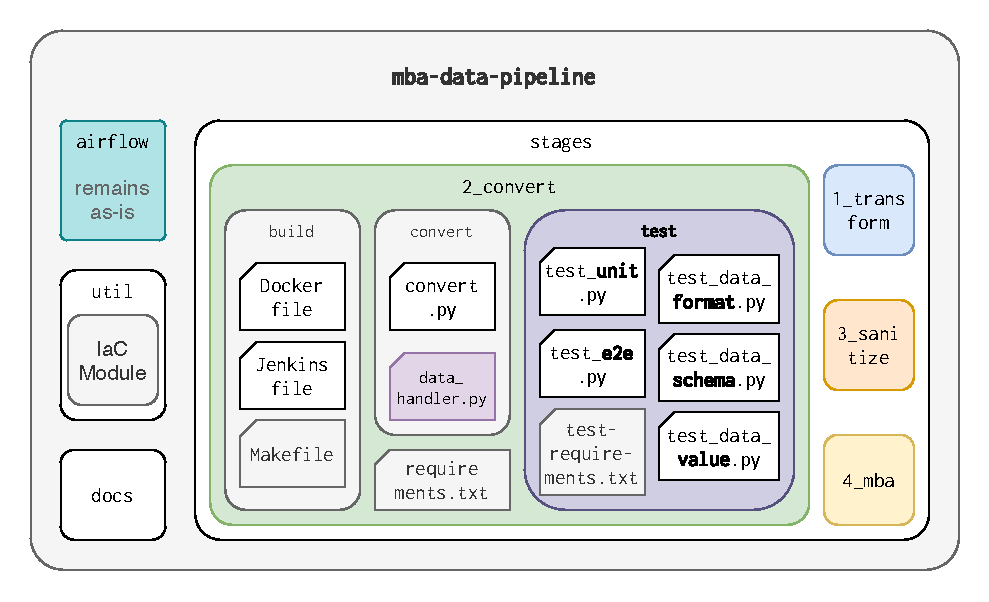
\includegraphics[width=\linewidth]{main-matter/img/5-repo-structure-new}
	\caption{Revisited Project Repository Structure (Testing Included)}
	\label{fig:5-new-repo}
\end{figure}

Figure \ref{fig:5-new-repo} visualizes the testing-enabled repository. Each stage receives its own \texttt{test} directory. This directory contains all testing class files as well as a requirements document, specifying required external installation for testing purposes. This document is similar to the already existing \texttt{requirements.txt} file.

With this change, Jenkins has now got access to the testing classes. Since the current Dockerfile already includes the entire stage module inside the image, the tests can already be run inside virtual Docker containers, which is desired. Currently, Jenkins only holds the production-grade \ac{iam} credentials inside is credential storage. The previously created \ac{iam} testing roles need to be added as well. Finally, the Jenkinsfile can be manipulated in order to provide appropriate testing stages inside the process, resulting in the pipeline depicted in Figure \ref{fig:5-cicd-testing}

\begin{figure}[h!]
	\centering
	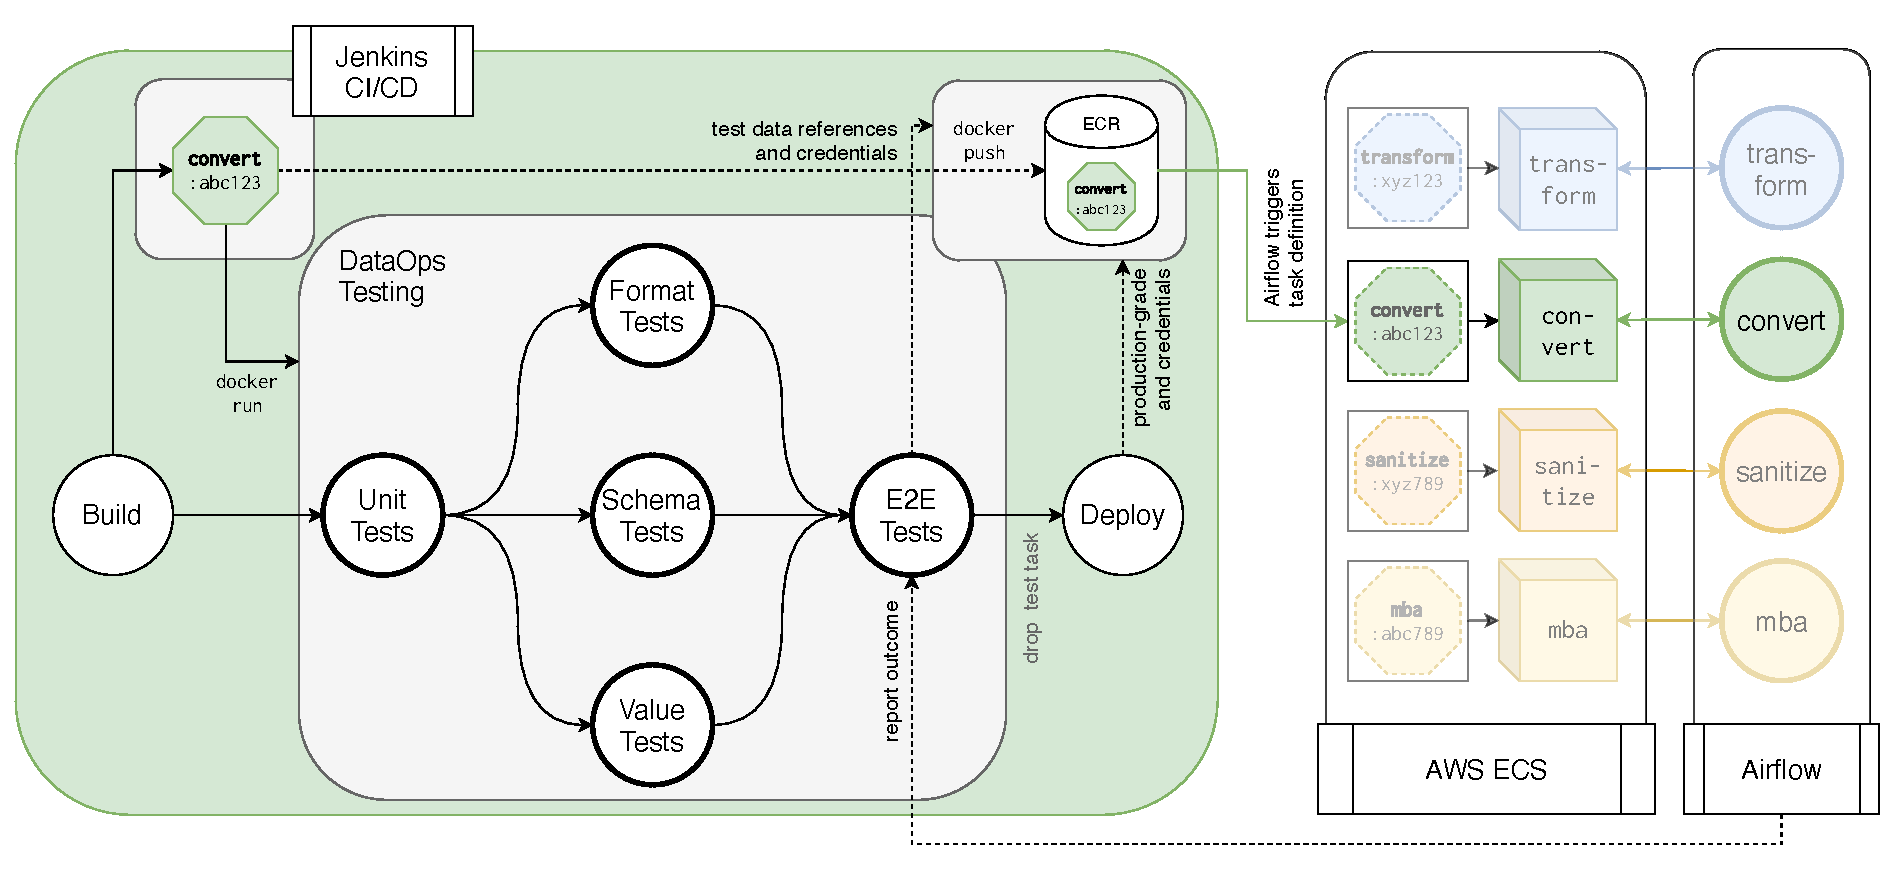
\includegraphics[width=\linewidth]{main-matter/img/5-cicd-testing.pdf}
	\caption{Testing-Enabled \acs{cicd} Pipeline Overview}
	\label{fig:5-cicd-testing}
\end{figure}

The build stage is changed such that the image is built with testing credentials rather than production-grade credentials. Additionally, Jenkins already specifies the test data locations during the image build process. In production, Airflow configures the required data location environment variables inside the task definition. With testing, Jenkins uses the unique Git commit identifier to define the data test job inside the \ac{s3} data lake. Then, testing stages are implemented. Their individual structures are very similar to each other. The testing stages of the Jenkinsfile are specified in Source Code Excerpt \ref{src:5-new-jenkinsfile-test}.

The unit testing stage calls the corresponding unit testing class file (l. 13) when running the Docker container (ll. 9--15). Additionally, a host-to-container volume mount is performed (l. 10) such that Jenkins receives access to the testing report file (l. 14). This file is used to display the testing report inside the Jenkins \ac{ui}. The integration (data) tests are implemented similarly, but run in parallel (l. 24--30). This does not cause any problems since these tests are run in entirely separate containers. The end-to-end test performs a pre-deployment prior to test execution (ll. 35--40). This is required because the test calls the Airflow \acs{api} to execute a test data pipeline including the new version image.

\begin{listing}[h!]
	\inputminted{groovy}{main-matter/src/5-new-jenkinsfile-test}
	\caption{Testing Stages of the Revisited Jenkinsfile}
	\label{src:5-new-jenkinsfile-test}
\end{listing}

Finally, the test deployment is removed and the actual deployment, including production-grade credentials and no data location specification, is performed. The environment changes (i.e., data lake structure and additional \ac{iam} role definitions) are added to the \ac{iac} process of the project. In case of an infrastructure rebuild, these components will be also generated and embedded automatically.

This concludes the implementation task which is now subject to evaluation.



		
	\chapter{Solution Evaluation}
		\label{chap:solution-evaluation}
		%===========================================================================
%	VI. Solution Evaluation
%===========================================================================

The following evaluation is expected to provide insights whether the solution works as intended during implementation. A focus is set on the testing capabilities of the \ac{cicd} pipeline in order to find potential limitations of the solution and discuss possible improvement techniques in theory. Throughout the evaluation, DataOps is compared to DevOps while focussing on the \ac{cicd} process and its testing features. This ultimately includes bottlenecks that cannot be covered by automated measures of the pipeline but rather need to be handled via conventions and best practices.

\section{Workflow Demonstration}
First of all, it might be valuable to evaluate the basic functionality of the \ac{cicd} pipeline, including its testing and deployment capabilities when no errors occur. For this matter, the general development workflow is applied. Before the following changes, the latest production-grade image was tagged with the commit ID \texttt{3c75dd5} inside \ac{ecr}.

A developer makes an arbitrary change to the Conversion Stage source code of the solution that is expected not to break the solution. This change is made in a separate feature branch of the \ac{vcs}. The developer can verify this fact by running the preexisting, automated tests locally on the developer sandbox. Then, a pull request is filed with the goal to merge the feature branch with the \texttt{master} branch, resulting in the new source code version being deployed into production. The pull request needs to include the appropriate GitHub labels, marking that the pull request should be treated as a new feature inside the Conversion \ac{cicd} pipeline. The filing could look like the screenshot provided in Figure \ref{fig:6-pr}. A pull request description is well-desired but omitted here for the sake of simplicity.
\newpage
\begin{figure}[h!]
	\centering
	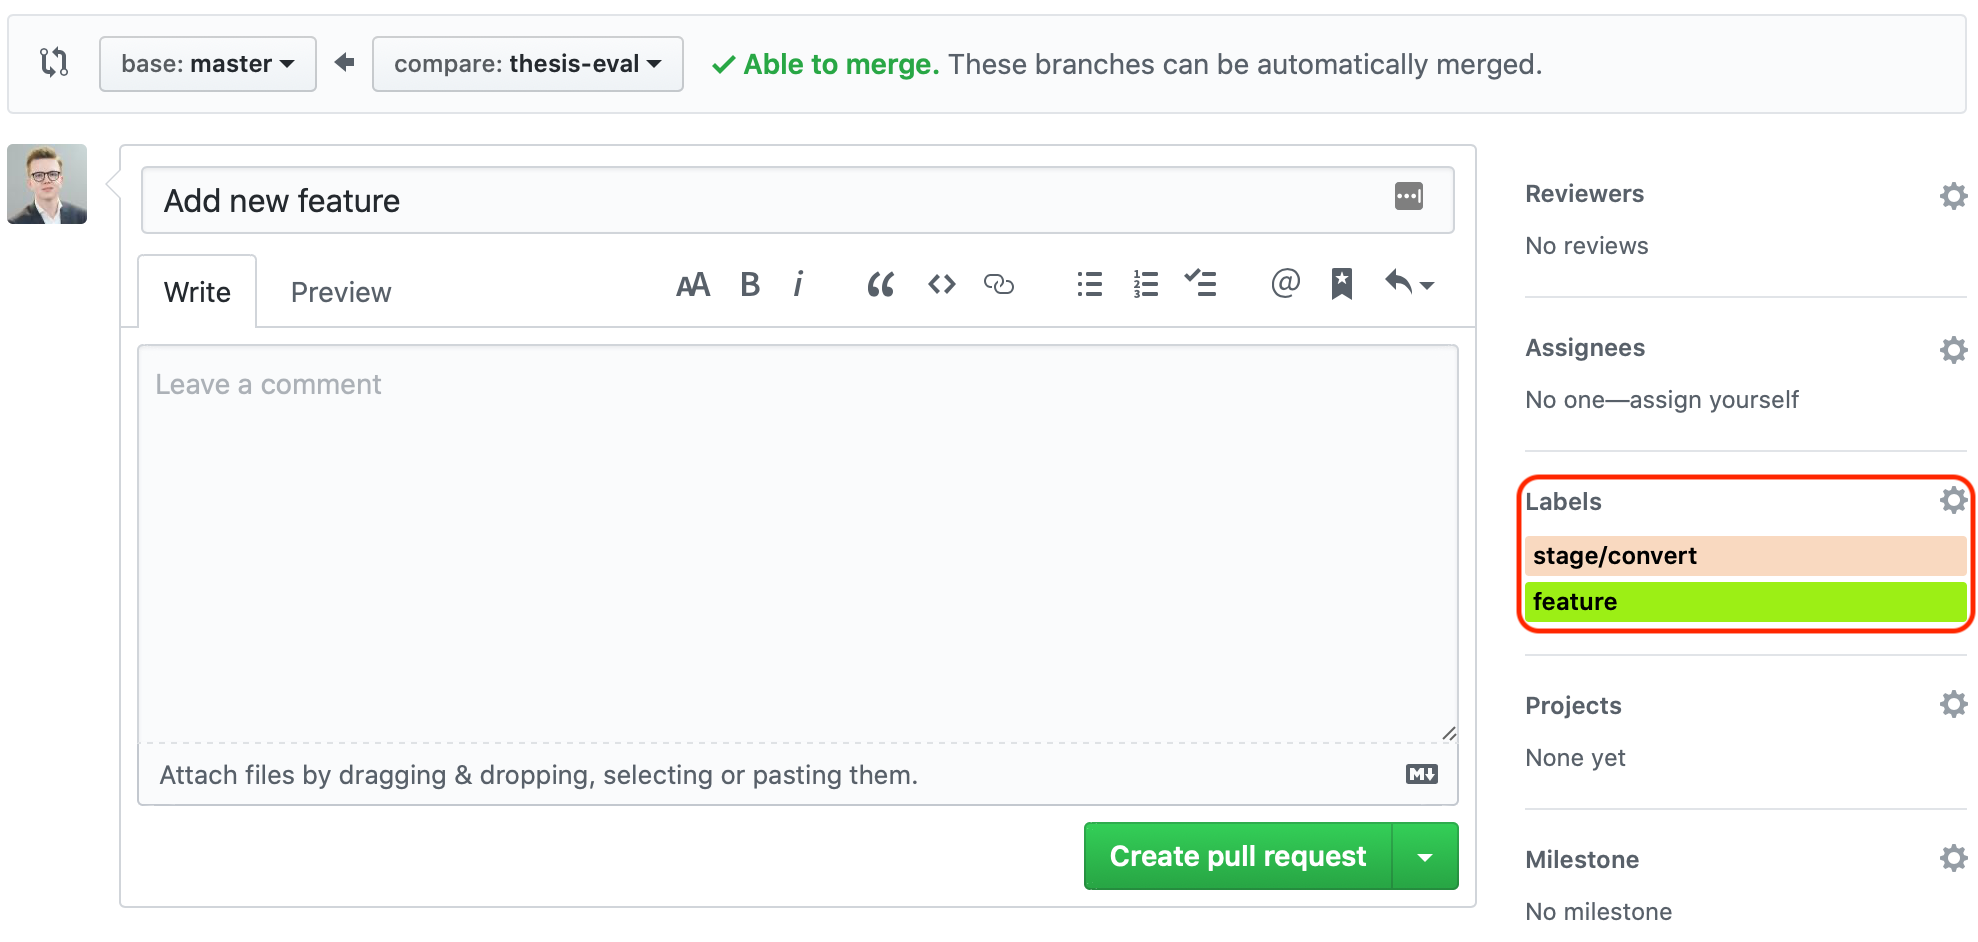
\includegraphics[width=\linewidth]{main-matter/img/6-pr.png}
	\caption{GitHub Feature Pull Request for Conversion Stage (Screenshot)}
	\label{fig:6-pr}	
\end{figure}

The first minor issue can be found inside this workflow. The developer in charge of this pull request is required to set the appropriate labels. The \texttt{feature} label missing would cause the \ac{cicd} pipeline not to run. The same applies to the stage specification label. An incorrect label could cause even more problems since this would trigger another pipeline with this stage source code, resulting in the build phase failing. The problem could be resolved by splitting up the repositories by stage but would remove the overall availability of the entire project's source code. This could have a negative impact on the productivity of the teams working on the project.

In case of correctly chosen labels, the Conversion Stage pipeline is triggered. A new pull request is automatically added to Jenkins and can be seen in the corresponding overview of the Jenkins \acs{ui}, shown in the screenshot in Figure \ref{fig:6-jenkins-pr}.

\begin{figure}[h!]
	\centering
	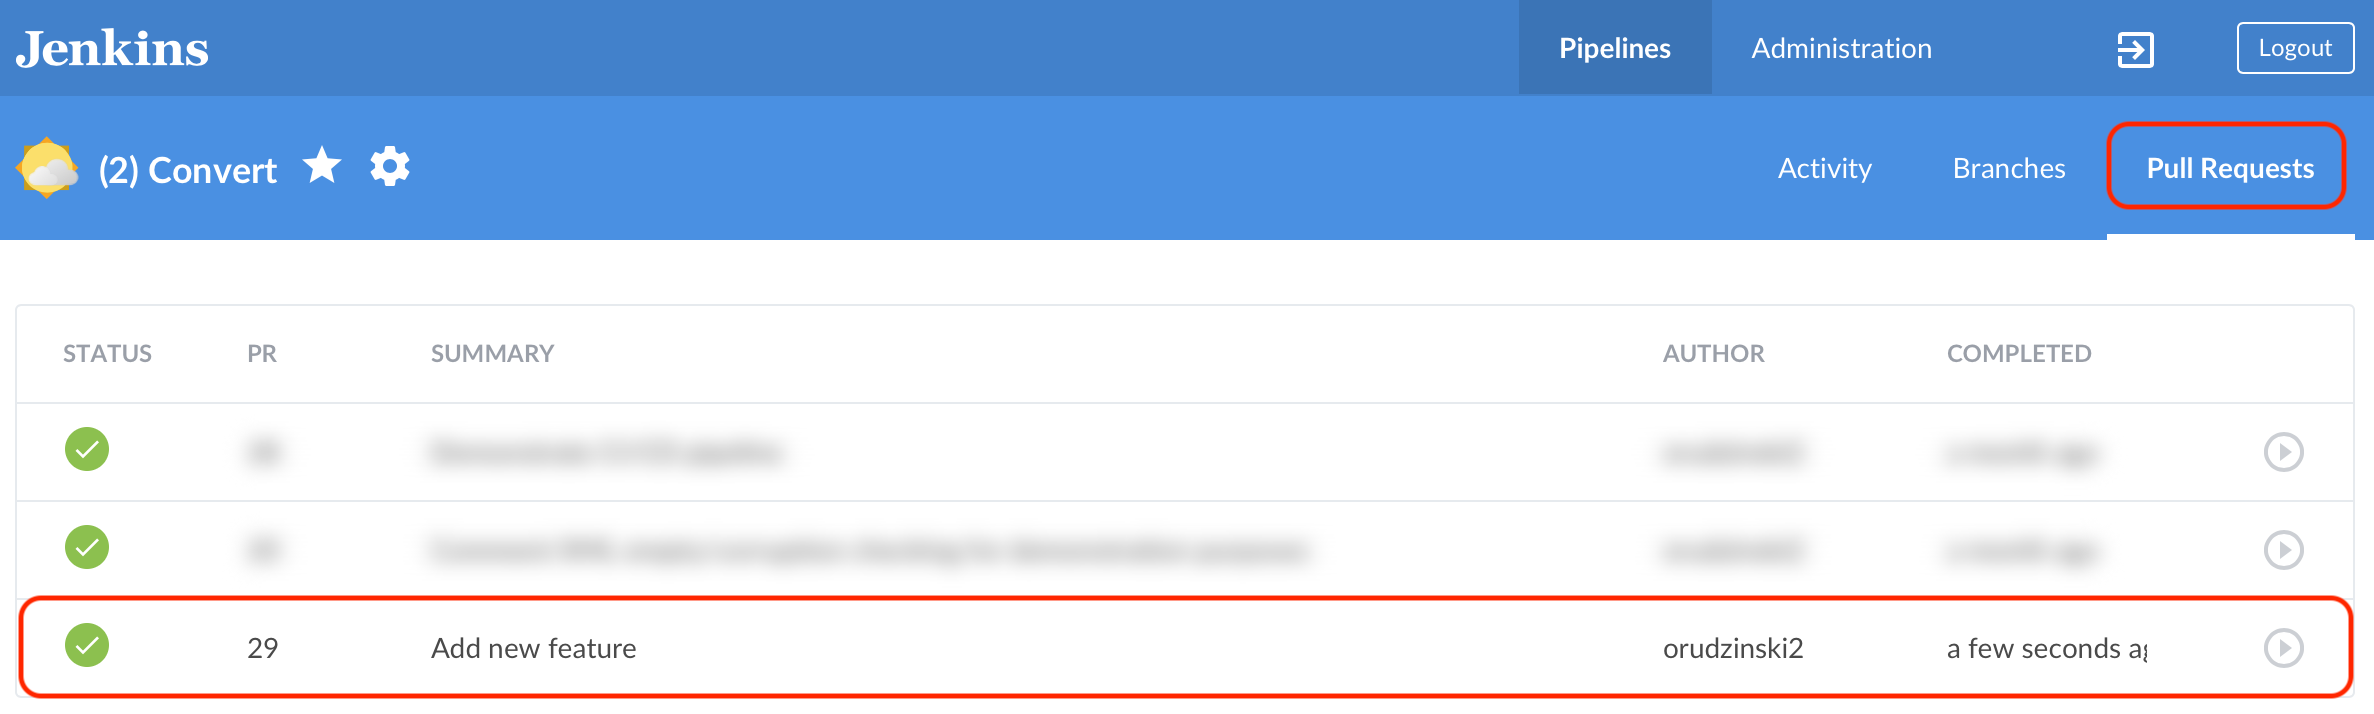
\includegraphics[width=\linewidth]{main-matter/img/6-jenkins-pr}
	\caption{Pull Request in Jenkins \acs{ui} (Screenshot)}
	\label{fig:6-jenkins-pr}
\end{figure}

The green checkmark shows that the pull request was evaluated, successfully verified and deployed. The specific pipeline overview can be retrieved by inspecting the corresponding pull request. This yields the following screenshot in Figure \ref{fig:6-jenkins-job-success}.

\begin{figure}[h!]
	\centering
	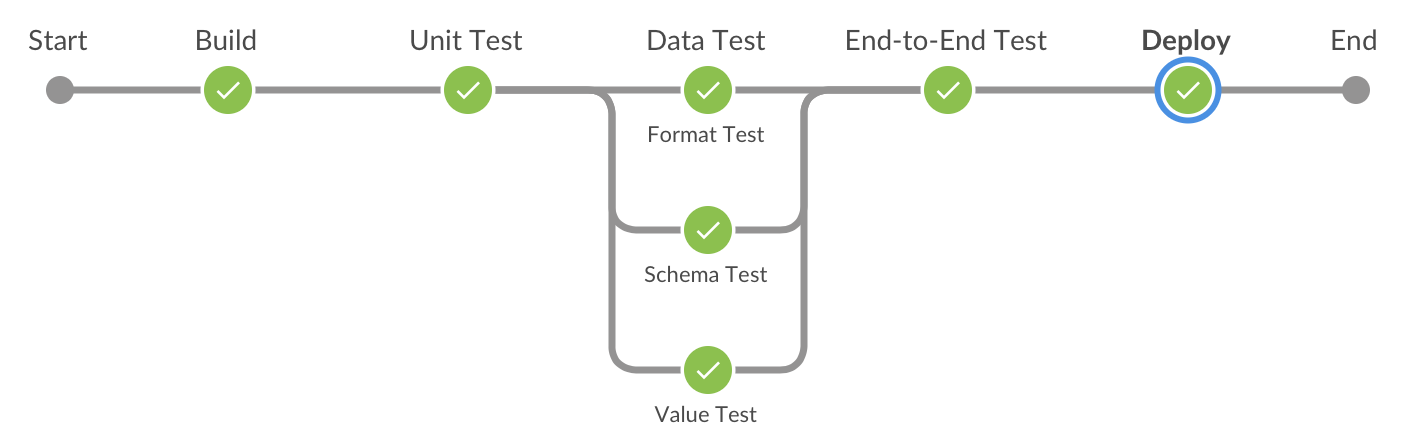
\includegraphics[width=\linewidth]{main-matter/img/6-jenkins-job-success}
	\caption{Successful Pipeline Job in Jenkins \acs{ui} (Screenshot)}
	\label{fig:6-jenkins-job-success}
\end{figure}

Since the deployment has run through correctly, \ac{ecr} should have received a new image. This image should be tagged with the last commit ID of the pull request as well as the \texttt{latest} tag. Inspecting the corresponding repository inside the \ac{aws} Console verifies this claim, presented in the screenshot of Figure \ref{fig:6-ecr}

\begin{figure}[h!]
	\centering
	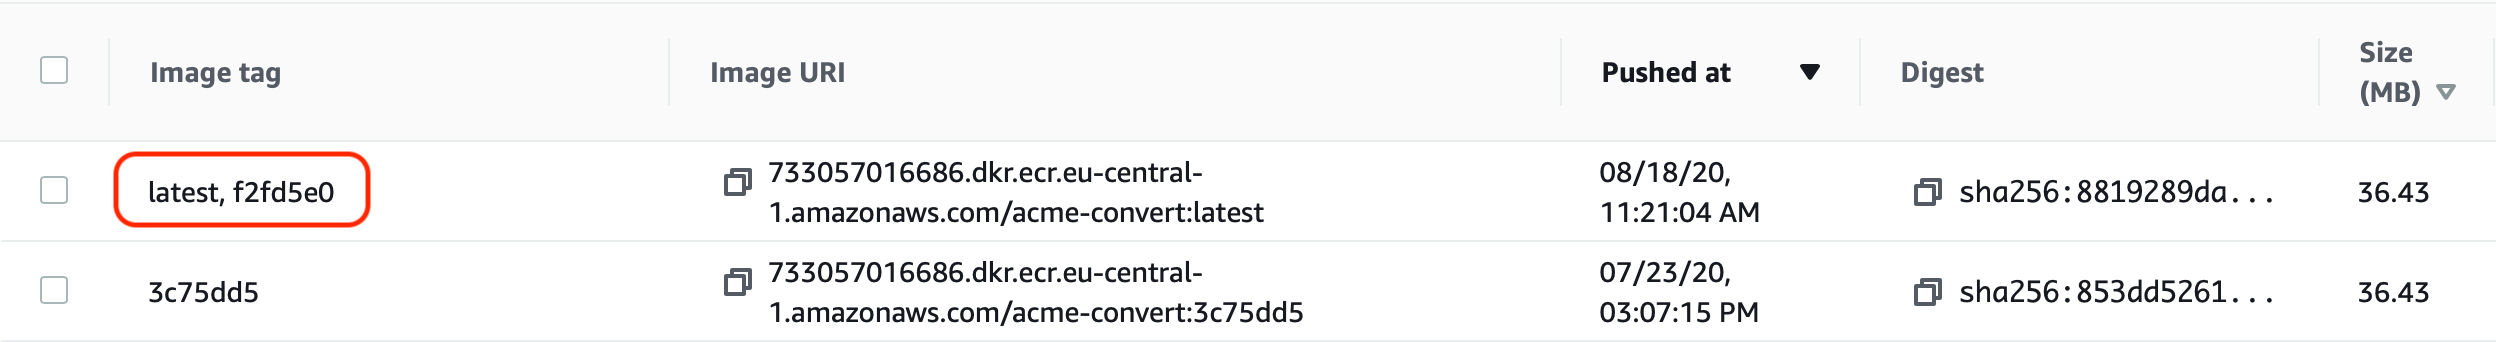
\includegraphics[width=\linewidth]{main-matter/img/6-ecr}
	\caption{Image List of the Conversion Stage \acs{aws} \acs{ecr} Repository (Screenshot)}
	\label{fig:6-ecr}
\end{figure}

It can be seen, that the new image has been included with the appropriate tags. The old version of the image still resides in the repository for versioning reasons. Because of the correct tagging, Airflow will use this updated version of the Conversion Stage image for upcoming analyses. 

The source code change is not reflected in the GitHub repository, yet. The feature branch still exists and the \texttt{master} branch has not been changed. Since the required \ac{cicd} checks have run through successfully, the developer can now merge the feature branch with the \texttt{master} branch. This manual procedure is required by GitHub. This can be seen as another issue of lacking automation since the developer may not forget to merge the branches and remove the feature branch after the deployment has been conducted successfully. Existing copies of the previous \texttt{master} branch inside other development sandboxes need to be updated now since working with the outdated version might cause compatibility issues of upcoming versions as well as so-called \textit{merge conflicts} within GitHub, where the feature might be correct by means of the \ac{cicd} evaluation, but the code history of the branches to merge does not allow for an automatic merge and requires manual correcting.

At this point, one iteration of the \ac{cicd} workflow is completed.

\section{Testing Capability Evaluation}
The previous evaluation use case does intentionally not contain issues in order to demonstrate the desired development workflow. Now, the workflow of the pipeline is evaluated for different kinds of issues. In general, this is divided into two categories:

\begin{enumerate}
	\item issues that result from updating existing features, and
	\item issues that result from creating new features.
\end{enumerate}

\subsection{Feature Update Testing}
The most na\"ive approach is to remove a line of code that is required by the testing framework. This simulation is comparable to a scenario where an existing feature is updated but a required functionality was removed. The testing framework is supposed to be invoked by the \ac{cicd} pipeline job and catch the issue. Specifically, the line checking for a corrupted \ac{xml} file inside the analytics script of the Conversion Stage is removed. This data handling function has been presented in Section \ref{sec:5-3-3-2}.

The process of filing a pull request remains identical. Jenkins' pull request job is triggered again, resulting in the job workflow depicted in the screenshot in Figure \ref{fig:6-jenkins-pr-fail1}.

\begin{figure}[h!]
	\centering
	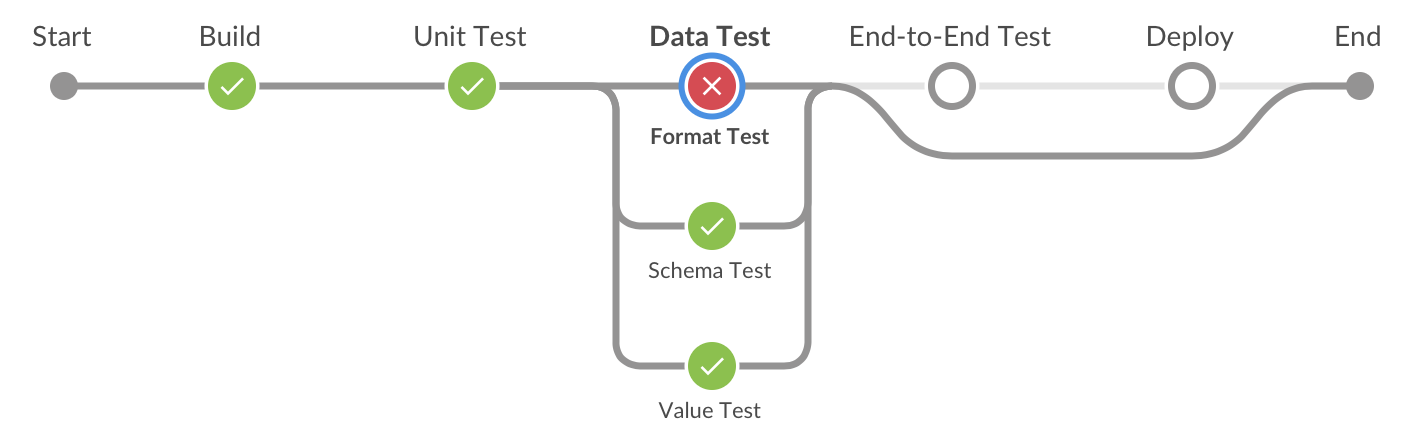
\includegraphics[width=\linewidth]{main-matter/img/6-jenkins-pr-fail1}
	\caption{Failing Pipeline Job in Jenkins \acs{ui} (Line Missing) (Screenshot)}
	\label{fig:6-jenkins-pr-fail1}
\end{figure}

Since \ac{xml} corruption testing is subject to the data format testing suite, the corresponding stage inside the \ac{cicd} pipeline fails. The upcoming stages are skipped such that no flawed deployment is conducted. The \textit{Tests} tab of the job inside the Jenkins \ac{ui} provides insights to the tests that have been run during the testing stages and highlights tests that did not pass. This overview is shown in a screenshot in Figure \ref{fig:6-jenkins-tests}.
\newpage
\begin{figure}[h!]
	\centering
	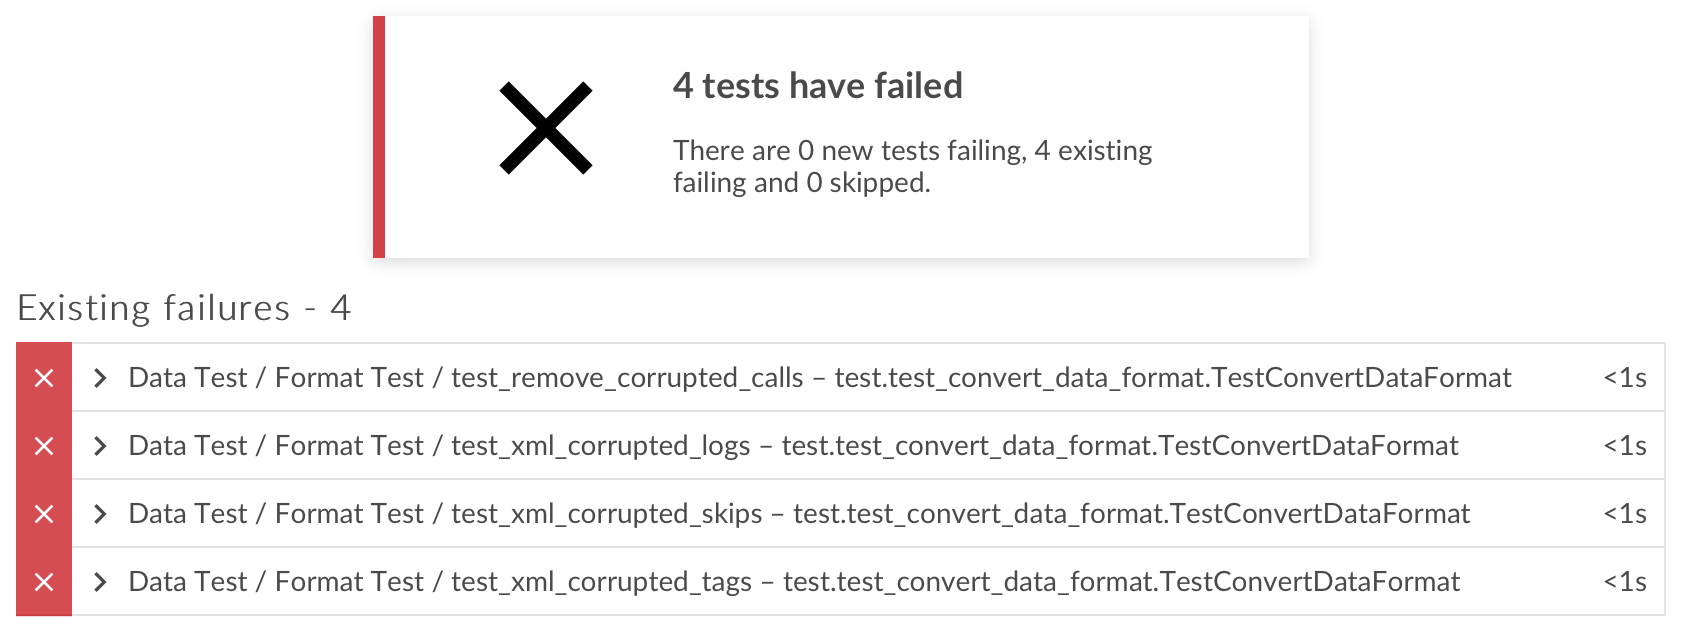
\includegraphics[width=\linewidth]{main-matter/img/6-jenkins-tests}
	\caption{Failing Tests in Jenkins \acs{ui} (Line Missing) (Screenshot)}
	\label{fig:6-jenkins-tests}
\end{figure}

It can be seen that all tests regarding \ac{xml} corruption fail. This is because the centralized \texttt{remove\_corrupted(...)} data handling function is not called inside the analytics script anymore. Since all handling measures are defined in that function, no measure is actually taken when the function call is missing. In case of the data handling function missing individual handling steps, the corresponding tests would fail. These test results are meant to provide valuable insights to the developer. The developer can analyze the problem, fix occurrences, and push a new commit to the pull request. When the test failures have been resolved, the updated version can be correctly deployed.

Similar failure detections occur with different changes of the source code. This shows that the pipeline is capable of stopping a deployment process based on the existing tests. This requires the assumption that all tests suites are complete and perform as expected.

\subsection{Feature Creation Testing}
The previous paragraphs cover the integration of an already existing feature. The following paragraphs deal with the creation and adequate testing of a new feature. The consideration of this practical area is important since the solution at hand can encounter changing requirements that need to be embodied accordingly.

For this evaluation, assume that the product owner of the \ac{mba} data pipeline requests a new feature that includes the weather data of the creation date of the purchase information to the analysis. This could be used to find a possible correlation between the purchasing behavior of the retail company's customers and the weather situation at the given point in time. The development teams find that the integration of weather data is mostly suited to be developed inside the Conversion Stage of the data pipeline since it represents the first stage that has access to the raw purchasing data.

The na\"ive implementation of that feature is shown in Source Code Excerpt \ref{src:6-weather} below.

\begin{listing}[h!]
	\inputminted{python}{main-matter/src/6-weather.py}
	\caption{Na\"ive Implementation of a Weather Data Integration Feature}
	\label{src:6-weather}
\end{listing}

The feature's corresponding function is placed right after the reformatting of the \ac{pos}Log dictionaries and, thus, right before the \ac{json} file export. For each purchase, the weather that corresponds to the transaction date and place is requested from an external weather \acs{api} (ll. 5--12). For simplicity reasons, the average weather data in degrees Celsius is extracted (ll. 14--16) and added to the dictionary (l. 18). There are multiple issues that can occur when such a code fragment is integrated to the solution. 

\subsubsection{Feature Testing Limitations}
When performing an update of an existing feature, the validation of the update can be conducted by running the preexisting tests of the corresponding feature. However, the development of a new feature also means writing new tests. The \ac{cicd} pipeline can only stop a feature from being deployed into production when corresponding feature tests fail. In case that these tests do not exist, the \ac{cicd} pipeline cannot recognize any issues and publishes an untested feature. This situation is highly undesired and problematic for the integrity of such a solution. Plus, it yields discussions that go beyond the technical aspects of data analytics development but need to deal with the developer's understanding and acceptance of an agile development workflow.

In agile development, a developer is always in charge of testing the feature that he or she works on \cite[18]{Kaiser}. Principles like \ac{tdd} have been introduced to support the importance of the testing process \cite[1]{Karac2018}. DataOps testing principles might develop this into a data-driven approach (i.e., test data first, then solution test, then feature implementation). Nevertheless, from a general point of view, these principles can be suggested or required by convention, but not technically enforced. A separate tool could evaluate if tests exist for a given feature by executing all test suites and calculating the feature's occurrences in these tests. This measurement is referred to as the \textit{test code coverage} \cite[15]{Garrett2011}. However, such a mechanism could be bypassed by simply executing a function inside a test case. This could presume the feature being tested and allow the change to be deployed into production. Other, more complex metrics (e.g., defect fix retest, test effectiveness, etc. \cite[15]{Garrett2011}) could be suited for more in-depth testing quality assurance, but would still be required to be implemented and reevaluated for the given use cases over time.  All in all, DataOps requires the acceptance and consciousness of agile processes and does not only rely on technical measurements to control their fulfillment.

Even with appropriate testing, the issue is still present. This is because the feature and the corresponding tests are conducted by human developers. The person behind a feature might have a different understanding of the feature than the product owner or simply miss an edge case during testing that could lead to further issues. Specifically, the developer might implement the feature to provide weather data in degrees Fahrenheit and test the value correctness accordingly. The product owner or other developers might expect degrees Celsius instead. As with pure software development, such a feature change also requires updating the solution requirements and general collaboration and communication between developers and development teams of the separate stages. In general, all contributors should have the same understanding of a feature in order to prevent inconsistencies.

This issue also introduces the discussion of \textit{testing tests} that are meant to test the functionality of the source code. The addition of testing validation based on previously mentioned complex testing quality metrics might mean more effort. With these validation systems, the question behind \textit{their} validity can be posed and the discussion continues. This ultimately means that automated tests might not suffice for confident and correct deployment of such a solution. Apart from that, peer code reviews and other interdisciplinary measures might need to be taken in order to rule out mistakes that cannot be uncovered by traditional software solution testing.

\subsubsection{Importance of Regression Testing}
Another issue can be found in regression. Assume that a previous \ac{mba} needs to be re-conducted because an error inside its values is suspected. The data from the target \ac{mba} originates from a time before this feature was requested. The previous \ac{mba} did also not consider weather data for its analysis. When the analysis is repeated, the \ac{mba} might, purposefully, yield different results. However, this behavior is not desired. The addition of a new feature shall not lead to inconsistencies between two versions of the same analysis. This would create a new data quality issue and result in further issues in the upcoming analytical stages. Instead, this feature may only be used for new analyses (e.g. by specifying a minimum date that needs to be present in the input data). This behavior correctness needs to be ensured by including a corresponding test to the testing suite of the solution.

Another form of regression testing in this case is the execution of previous tests. Their passing will ensure that the new feature does not change the behavior of previously existing features. Since this feature only adds an attribute to the output of the stage, the previous features and feature tests run correctly. Other feature implementations might require the change of preexisting features which then might require the adaptation of the corresponding tests, etc. \\\

All in all, the general testing process, including its limitations and technical bottlenecks, can be compared to agile DevOps testing. On the other hand, regression testing plays a priority role in data analytics testing and needs to be taken into account for each feature. This finding preliminarily corresponds with the hypothesis from Section \ref{sec:2-2-innovation-pipeline}. Currently, it can be said that the DataOps testing process is similar to DevOps, but takes data-specific requirements into account.

\section{Impact Analysis of Different Testing Levels}
In order to evaluate further potential differences to the DevOps testing process, the following section deals with the different testing levels (unit, integration, and end-to-end testing) in the \ac{mba} DataOps pipeline environment. This part of the evaluation is expected to yield insights about the specific impact of the testing levels in such a data-driven environment, built up in a highly externalized technical infrastructure. 

This evaluation is conducted based on testing use cases that occur at different hierarchical levels of the testing process. These use cases are not explicitly tested for by the solution. The evaluation will provide information on how insightful the error recognition of the different testing levels is for recovering from the problem. The use cases are described as follows:

\begin{description}
	\item[Non-Existing \ac{s3} Bucket \acs{uri} Provided] The format of the \ac{uri} is correct, but the bucket does not exist (typographic error, deprecated bucket reference, etc.).
	\item[Invalid \ac{aws} \ac{iam} Credentials Provided] The format of the \ac{iam} credential key pair is correct, but it either does not provide sufficient access to the resources, or it is deprecated .
	\item[Container Task Ran Out of Memory] The container that an analytics stage is run in cannot finish its job because it requires more memory than expected.
\end{description}

\subsection{Failure Case Execution}
These cases are designed and invoked, leading to the following results:

\subsubsection{Non-Existing \ac{s3} Bucket \acs{uri} Provided}
\begin{table}[h!]
\centering
\begin{tabular}{r!{\vrule width 1pt}l|l|l}
\multicolumn{4}{c}{\textbf{Non-Existing \acs{s3} Bucket \acs{uri} Provided}}                                                                        \\[0.4em] \ChangeRT{1pt}
\makecell[r]{\textbf{Level}}       & \textbf{Unit} & \textbf{Integration}                                                       & \textbf{End-to-End} \\ \ChangeRT{1pt}
\makecell[r]{\textbf{Result}}      & \cellcolor{green!25}passed        & \cellcolor{red!25}failed                                                                     & \cellcolor{gray!25}\textit{skipped}                \\ \hline
\makecell[r]{\textbf{Information}} &               & \makecell[l]{\texttt{boto3} Exception:\\ \texttt{404 Not Found}} &                    
\end{tabular}
\caption{Testing Evaluation: Non-Existing \acs{s3} Bucket \acs{uri} Provided}
\label{tab:6-bad-s3}
\end{table}

As can be seen in Table \ref{tab:6-bad-s3}, the corresponding unit test only tests if \ac{s3} \acsp{uri} of incorrect format are caught and reported. Since the \acs{uri} at hand is correct, the unit test passes. The integration (data) test actually connects to the bucket, resulting in an \texttt{boto3} exception, reporting that the provided \ac{s3} bucket does not exist.

The process of mocking the \ac{s3} connection service inside the unit test would not have helped here since the actual existence of the infrastructure can only be evaluated \textit{within} the scope of the infrastructure.
\newpage
\subsubsection{Invalid \ac{aws} \ac{iam} Credentials Provided}
\begin{table}[h!]
\centering
\begin{tabular}{r!{\vrule width 1pt}l|l|l}
\multicolumn{4}{c}{\textbf{Invalid \ac{aws} \ac{iam} Credentials Provided}}                                                                        \\[0.4em] \ChangeRT{1pt}
\makecell[r]{\textbf{Level}}       & \textbf{Unit} & \textbf{Integration}                                                       & \textbf{End-to-End} \\ \ChangeRT{1pt}
\makecell[r]{\textbf{Result}}      & \cellcolor{green!25}passed        & \cellcolor{red!25}failed                                                                     & \cellcolor{gray!25}\textit{skipped}                \\ \hline
\makecell[r]{\textbf{Information}} &               & \makecell[l]{\texttt{boto3} Exception:\\ \texttt{Access Denied}} &                    
\end{tabular}
\caption{Testing Evaluation: Invalid \acs{aws} \acs{iam} Credentials Provided}
\label{tab:6-bad-iam}
\end{table}
This case is similar to the incorrect \acs{uri} and results in the same test outcome, shown in Table \ref{tab:6-bad-iam}. Only the infrastructure itself can evaluate the credentials and report an issue. This is why, again, the unit test passes, while the integration test results in another exception, mentioning that the provided credentials cannot be used for the current operation.

\subsubsection{\acs{ecs} Container Task Ran Out of Memory}
\begin{table}[h!]
\centering
\begin{tabular}{r!{\vrule width 1pt}l|l|l}
\multicolumn{4}{c}{\textbf{\acs{ecs} Container Task Ran Out of Memory}}                                                                        \\[0.4em] \ChangeRT{1pt}
\makecell[r]{\textbf{Level}}       & \textbf{Unit} & \textbf{Integration}                                                       & \textbf{End-to-End} \\ \ChangeRT{1pt}
\makecell[r]{\textbf{Result}}      & \cellcolor{green!25}passed        & \cellcolor{green!25}passed                                                                     & \cellcolor{red!25}failed                \\ \hline
\makecell[r]{\textbf{Information}} &               &  & \makecell[l]{\texttt{boto3} Exception:\\ \texttt{OutOfMemoryError: Container killed}\\\texttt{due to memory usage}}                  
\end{tabular}
\caption{Testing Evaluation: \acs{ecs} Container Task Ran Out of Memory}
\label{tab:6-oom}
\end{table}
In this case, both the unit and integration tests do not recognize the problem. Only the end-to-end test provides the information that the corresponding \ac{ecs} task has failed because of lacking memory capacity, shown in Table \ref{tab:6-oom} This is because the integration tests are performed in containerized environments on the Jenkins server instance. These Docker containers do not have any resource limitations \cite{docker}, in contrast to the \ac{ecs} tasks that require performance specifications in their definitions. Only the end-to-end test makes use of this infrastructural service inside the solution.
\newpage
\subsection{Testing Impact Evaluation}
The presented use cases yield a number of insights. First, the typical, DevOps-inspired testing level hierarchy and its degrees of testing isolation do not hold in an environment that is mostly created out of external resources. The cloud-driven infrastructure cannot be taken into account by unit tests since these are supposed to neglect these aspect and purely focus on the feature under test. When the infrastructure access is a crucial component of the feature, the unit test cannot recognize any issues.

Another aspect that follows is the strict separation of the testing levels. Taking the findings of the failure use cases into account, all infrastructure-related testing might be conducted during integration testing. This could also include \acs{uri} and \acs{iam} credential format tests that do not require infrastructure access but categorically fit inside the same testing suite. This aspect has partly been considered during development: certain data handling function tests could have been created in the domain of granular unit tests. Since their overall features relate to the data-driven part of the solution, which has been tested during integration testing, the remaining tests are performed similarly.

Finally, the last failure use case that was only recognized by end-to-end testing opens up another discussion topic. In general, the performance measures could have been implemented into the integration testing level that makes use of Jenkins-driven Docker containers. This would require additional testing effort and, potentially, the redesign of the deployment structure within the \ac{cicd} pipeline. While the overall reason behind testing should be the validation of feature functionality, strictly focussing on the definition of the testing levels could increase time and cost inside the development process.

As emphasized throughout this entire work, DataOps use cases and their corresponding automation and testing designs highly differ depending on the solution requirements, data governance definitions, etc. For the \ac{mba} data pipeline, unit tests provide little value to the actual testing expressiveness. There exists a general discussion questioning the value of unit tests \cite{Coplien}\cite{Golub2020}. This finding goes hand-in-hand with this discussion. On the other hand, unit testing allows for better testing performance. When the practice of \textit{mocking} external services (i.e., mimicking the required service functionality inside the local test case) is exhausted, this performance benefit vanishes due to increasing testing design complexity. The unit test cases might be included into the integration testing area and de-granularized for potentially better testing productivity. Further evaluation could give more insights on the impact differences between integration and end-to-end testing, leading to a generally more specialized, efficient and less tradition-driven testing architecture. 

All in all, it is proposed that DataOps tests are categorized semantically regarding their meaning for the solution rather than focussing on testing level syntax. Furthermore, testing design needs to be weighted up between the creation complexity of isolated tests as well as the urge for isolated unit test cases. \\\

In generalization and comparison to the DevOps testing process, it can still be said that automated testing is performed inside its designated steps inside the \ac{cicd} process prior to deployment. However, data analytics solutions often have to deal with externalized services, that cannot be neglected during testing. Instead of sticking to the traditional testing pyramid, each solutions' architecture needs to be evaluated from a testability point of view in order to create a well-suited testing framework inside the DataOps use case.




		
	\chapter{Conclusion}
		\label{chap:conclusion}
		%===========================================================================
%	VII. Conclusion
%===========================================================================

This final chapter retrospects on the work and findings inside this bachelor's thesis. It started out with background information on DataOps and testing methodologies. It conducted an actual state analysis of a preexisting, static \ac{mba} data analytics solution based on the state-of-the-art findings. This determined action items for the DataOps enablement and testing enhancement of the solution. The thesis then proposed a general DataOps testing framework and applied its steps on the Conversion Stage of the data pipeline in theory. Then, the DataOps process and testing framework have been practically implemented. Finally, the new solution was evaluated by means of the key goals of this thesis, being the understanding of DataOps testing, similarities and differences to DevOps testing, as well as limitation of the solution.

\section*{Key Findings} \addtocounter{section}{1}
During research, design, implementation, and evaluation, the following key characteristics were found:

As with traditional software solution testing, data analytics testing supports the quality of new version releases. It provides confidence in the product for all stakeholders, leading to less post-deployment issues, and therefore, to less cost, time, and risk during production-grade usage. Eventually, well-tested data analytics solutions are expected to provide more valuable business insights for the organizations that take advantage of them.

Moreover, DataOps testing is an inherent part of DataOps that benefits from technical support through automation and the separation of execution environments. Nevertheless, DataOps remains an agile work model that requires an adequate agile mindset. The DataOps \ac{cicd} pipeline can only recognize test failures with actually available tests. If a developer team decides to neglect testing and work around potential testing mechanisms, there will be no tests that could fail, resulting in a passing deployment. From a qualitative point of view, this is unacceptable but could not be realistically enforced with additional technical measures. Instead, testing conventions and best practices should be known and accepted by the performing developers. Then, DataOps testing can be very valuable for correct and confident solution development and deployment.

Even with the required agile mindset, test quality might be an issue. Since these tests are written by human developers, they might not take certain edge cases into account, leading to an insufficiently tested solution. Again, test quality measurements could be implemented into the solution but should also be supported by non-automated processes, like peer code reviews, etc.

The testing design process should consider that historic analyses might need to be re-conducted, aiming for consistent results regardless of the current version of the data analytics solution. Therefore, regression testing and the conditional execution of features need to be taken into account.

While DataOps testing can be achieved by utilizing traditional software testing tools, it does not follow the exact same process of DevOps testing. Since data analytics solutions often depend on a variety of external services, these also need to be considered during testing. This goes against the traditional testing pyramid that aims for isolated, granular unit tests. Instead, DataOps tests should not strictly stick to the traditional testing levels but provide semantically categorized testing suites that reflect the desired workflow of the solution.

\section*{Proposal for Further Research} \addtocounter{section}{1}
The preliminary goal of the thesis' project was to demonstrate the discipline of DataOps testing by means of an exemplarily chosen data analytics scenario. Throughout the research and development process, it became clear that different types of data analytics projects are expected to have different types of requirements. It might be reasonable to evaluate the testing design framework and process inside other use cases, using different technologies. For instance, it is expected that more complex, \acs{ml}-driven data analytics will require additional infrastructure and testing methodologies. Furthermore, analytics derived through \acs{ml} might need additional testing attention regarding ethical questions. In general, the solution at hand covers deterministic testing. It might be of great interest to find out how such testing is conducted with predictive data analytics. \newpage

Picking up on the test quality issue finding from this thesis, implementation and evaluation of test quality assurance measures might concretize if testing conventions can be reasonably supported by automated mechanisms. \\\

In conclusion, the demonstration of \ac{mba} DataOps testing underlined the importance and capability of data analytics development and testing automation. With further research and development based on this work, generally applicable DataOps testing frameworks and tools for a variety of use cases and complexities could be created, resulting in better data analytics solutions and outcomes for organizations throughout several industries.
		
	\newpage \clearpage \thispagestyle{empty} \null
		
%===========================================================================
%	BACK MATTER
%===========================================================================

	\pagestyle{plain}
	\clearpage
	\pagenumbering{alph}
	\printbibliography
	
	\newpage \clearpage \thispagestyle{empty} \null
	
	\appendix
	\chapter{Appendix} \label{app:root}
	\section{Conversion Stage Data Events} \label{app:data-events}

\captionsetup[table]{list=no}
\captionsetup[figure]{list=no}

\begin{table}[h!]
\centering
\begin{tabular}{r!{\vrule width 1pt}l}
\makecell[r]{\textbf{Description}} & \makecell[l]{\textbf{One or multiple \acs{xml} file(s) are not named based on unified} \\ \textbf{naming format}} \\ \ChangeRT{1pt}
	
\makecell[r]{\textbf{Category}}    & Data Format                         \\ \ChangeRT{0.5pt}
\makecell[r]{\textbf{Severity}}    & \texttt{WARNING}                               \\ \hline
\makecell[r]{\textbf{Handling}}    & \makecell[l]{
	1. Increase \texttt{WARNING} degree counter accordingly \\
	2. Calculate threshold difference, terminate if exceeded \\
	3. Flag file (\texttt{name-warn}) \\
	4. Log warning including file information \\
	5. Continue analytical process \\
}           
\end{tabular}
	\caption{Incorrect Input File Naming}
\end{table}

\begin{table}[h!]
\centering
\begin{tabular}{r!{\vrule width 1pt}l}
\makecell[r]{\textbf{Description}} & \makecell[l]{\textbf{One or multiple \acs{xml} file(s) do not have the} \\ \textbf{appropriate file extension \texttt{.xml}}} \\ \ChangeRT{1pt}
	
\makecell[r]{\textbf{Category}}    & Data Format                         \\ \ChangeRT{0.5pt}
\makecell[r]{\textbf{Severity}}    & \texttt{WARNING}                               \\ \hline
\makecell[r]{\textbf{Handling}}    & \makecell[l]{
	1. Increase \texttt{WARNING} degree counter accordingly \\
	2. Calculate threshold difference, terminate if exceeded \\
	3. Flag file (\texttt{ext-warn}) \\
	4. Log warning including file information \\
	5. Continue analytical process \\
}           
\end{tabular}
	\caption{Incorrect Input File Extension}
\end{table}

\begin{table}[h!]
\centering
\begin{tabular}{r!{\vrule width 1pt}l}
\makecell[r]{\textbf{Description}} & \makecell[l]{\textbf{One or multiple \acs{xml} file(s) are empty}} \\ \ChangeRT{1pt}
	
\makecell[r]{\textbf{Category}}    & Data Format                         \\ \ChangeRT{0.5pt}
\makecell[r]{\textbf{Severity}}    & \texttt{ERROR}                               \\ \hline
\makecell[r]{\textbf{Handling}}    & \makecell[l]{
	1. Remove empty file from analysis \\
	2. Increase \texttt{ERROR} degree counter accordingly \\
	3. Calculate threshold difference, terminate if exceeded \\
	4. Flag file (\texttt{empty-err}) \\
	5. Log error including file information \\
	6. Continue analytical process \\
}           
\end{tabular}
	\caption{Empty Input File}
\end{table}

\begin{table}[h!]
\centering
\begin{tabular}{r!{\vrule width 1pt}l}
\makecell[r]{\textbf{Description}} & \makecell[l]{\textbf{One or multiple \acs{xml} file(s) not of \ac{pos}Log format}} \\ \ChangeRT{1pt}
	
\makecell[r]{\textbf{Category}}    & Data Format                         \\ \ChangeRT{0.5pt}
\makecell[r]{\textbf{Severity}}    & \texttt{ERROR}                               \\ \hline
\makecell[r]{\textbf{Handling}}    & \makecell[l]{
	1. Remove incompatible file from analysis \\
	2. Increase \texttt{ERROR} degree counter accordingly \\
	3. Calculate threshold difference, terminate if exceeded \\
	4. Flag file (\texttt{noPoslog-err}) \\
	5. Log error including file information \\
	6. Continue analytical process \\
}           
\end{tabular}
	\caption{Incompatible (i.e., Non-\ac{pos}Log) File}
\end{table}

\begin{table}[h!]
\centering
\begin{tabular}{r!{\vrule width 1pt}l}
\makecell[r]{\textbf{Description}} & \makecell[l]{\textbf{One or multiple \acs{xml} file(s) are missing required} \\ \textbf{global attribute(s)}} \\ \ChangeRT{1pt}
	
\makecell[r]{\textbf{Category}}    & Data Schema                         \\ \ChangeRT{0.5pt}
\makecell[r]{\textbf{Severity}}    & \texttt{ERROR}                               \\ \hline
\makecell[r]{\textbf{Handling}}    & \makecell[l]{
	1. Remove incorrect file from analysis \\
	2. Increase \texttt{ERROR} degree counter accordingly \\
	3. Calculate threshold difference, terminate if exceeded \\
	4. Flag file (\texttt{glbAttr-err}) \\
	5. Log error including file information \\
	6. Continue analytical process \\
}           
\end{tabular}
	\caption{Input File Missing Required Global Attribute(s)}
\end{table}

\begin{table}[h!]
\centering
\begin{tabular}{r!{\vrule width 1pt}l}
\makecell[r]{\textbf{Description}} & \makecell[l]{\textbf{One or multiple \ac{xml} file(s) have insufficient number} \\ \textbf{of item purchases}} \\ \ChangeRT{1pt}
	
\makecell[r]{\textbf{Category}}    & Data Schema                         \\ \ChangeRT{0.5pt}
\makecell[r]{\textbf{Severity}}    & \texttt{ERROR}                               \\ \hline
\makecell[r]{\textbf{Handling}}    & \makecell[l]{
	1. Remove incorrect file from analysis \\
	2. Increase \texttt{ERROR} degree counter accordingly \\
	3. Calculate threshold difference, terminate if exceeded \\
	4. Flag file (\texttt{item-err}) \\
	5. Log error including file information \\
	6. Continue analytical process \\
}           
\end{tabular}
	\caption{Insufficient Item Purchases in Input File}
\end{table}

\begin{table}[h!]
\centering
\begin{tabular}{r!{\vrule width 1pt}l}
\makecell[r]{\textbf{Description}} & \makecell[l]{\textbf{One or multiple \acs{xml} file(s) are missing required} \\ \textbf{item purchase attribute(s)}} \\ \ChangeRT{1pt}
	
\makecell[r]{\textbf{Category}}    & Data Schema                         \\ \ChangeRT{0.5pt}
\makecell[r]{\textbf{Severity}}    & \texttt{ERROR}                               \\ \hline
\makecell[r]{\textbf{Handling}}    & \makecell[l]{
	1. Remove incorrect file from analysis \\
	2. Increase \texttt{ERROR} degree counter accordingly \\
	3. Calculate threshold difference, terminate if exceeded \\
	4. Flag file (\texttt{itemAttr-err}) \\
	5. Log error including file information \\
	6. Continue analytical process \\
}           
\end{tabular}
	\caption{Input File Missing Required Item Purchase Attribute(s)}
\end{table}

\begin{table}[h!]
\centering
\begin{tabular}{r!{\vrule width 1pt}l}
\makecell[r]{\textbf{Description}} & \makecell[l]{\textbf{One or multiple \acs{xml} file(s) are missing optional} \\ \textbf{item purchase attribute(s)}} \\ \ChangeRT{1pt}
	
\makecell[r]{\textbf{Category}}    & Data Schema                         \\ \ChangeRT{0.5pt}
\makecell[r]{\textbf{Severity}}    & \texttt{WARNING}                               \\ \hline
\makecell[r]{\textbf{Handling}}    & \makecell[l]{
	1. Increase \texttt{WARNING} degree counter accordingly \\
	2. Calculate threshold difference, terminate if exceeded \\
	3. Flag file (\texttt{itemAttr-warn}) \\
	4. Log warning including file information \\
	5. Continue analytical process \\
}           
\end{tabular}
	\caption{Input File Missing Optional Item Purchase Attribute(s)}
\end{table}

\begin{table}[h!]
\centering
\begin{tabular}{r!{\vrule width 1pt}l}
\makecell[r]{\textbf{Description}} & \makecell[l]{\textbf{One or multiple \acs{xml} file(s) are missing required} \\ \textbf{sale information attribute(s)}} \\ \ChangeRT{1pt}
	
\makecell[r]{\textbf{Category}}    & Data Schema                         \\ \ChangeRT{0.5pt}
\makecell[r]{\textbf{Severity}}    & \texttt{ERROR}                               \\ \hline
\makecell[r]{\textbf{Handling}}    & \makecell[l]{
	1. Remove incorrect file from analysis \\
	2. Increase \texttt{ERROR} degree counter accordingly \\
	3. Calculate threshold difference, terminate if exceeded \\
	4. Flag file (\texttt{saleAttr-err}) \\
	5. Log error including file information \\
	6. Continue analytical process \\
}           
\end{tabular}
	\caption{Input File Missing Required Sale Information Attribute(s)}
\end{table}

\begin{table}[h!]
\centering
\begin{tabular}{r!{\vrule width 1pt}l}
\makecell[r]{\textbf{Description}} & \makecell[l]{\textbf{One or multiple \acs{xml} file(s) are missing optional} \\ \textbf{sale information attribute(s)}} \\ \ChangeRT{1pt}
	
\makecell[r]{\textbf{Category}}    & Data Schema                         \\ \ChangeRT{0.5pt}
\makecell[r]{\textbf{Severity}}    & \texttt{WARNING}                               \\ \hline
\makecell[r]{\textbf{Handling}}    & \makecell[l]{
	1. Increase \texttt{WARNING} degree counter accordingly \\
	2. Calculate threshold difference, terminate if exceeded \\
	3. Flag file (\texttt{saleAttr-warn}) \\
	4. Log warning including file information \\
	5. Continue analytical process \\
}           
\end{tabular}
	\caption{Input File Missing Optional Sale Information Attribute(s)}
\end{table}

\begin{table}[h!]
\centering
\begin{tabular}{r!{\vrule width 1pt}l}
\makecell[r]{\textbf{Description}} & \makecell[l]{\textbf{Date in file name does not correspond with \acs{xml} date attribute} \\ \textbf{sale information attribute(s)}} \\ \ChangeRT{1pt}
	
\makecell[r]{\textbf{Category}}    & Data Schema                         \\ \ChangeRT{0.5pt}
\makecell[r]{\textbf{Severity}}    & \texttt{CRITICAL}                               \\ \hline
\makecell[r]{\textbf{Handling}}    & \makecell[l]{
	1. Log error including data information \\
	2. Prompt error information \\
	3. Terminate analytical process
}           
\end{tabular}
	\caption{Input File Name Date Not Corresponding With \acs{xml} Date Attribute}
\end{table}

\begin{table}[h!]
\centering
\begin{tabular}{r!{\vrule width 1pt}l}
\makecell[r]{\textbf{Description}} & \makecell[l]{\textbf{Formatted Python Dictionary is missing} \\ \textbf{file-equivalent attribute(s)}} \\ \ChangeRT{1pt}
	
\makecell[r]{\textbf{Category}}    & Data Schema                         \\ \ChangeRT{0.5pt}
\makecell[r]{\textbf{Severity}}    & \texttt{CRITICAL}                               \\ \hline
\makecell[r]{\textbf{Handling}}    & \makecell[l]{
	1. Log error including data information \\
	2. Prompt error information \\
	3. Terminate analytical process
}           
\end{tabular}
	\caption{Formatted Python Dictionary Missing Attribute(s)}
\end{table}

\begin{table}[h!]
\centering
\begin{tabular}{r!{\vrule width 1pt}l}
\makecell[r]{\textbf{Description}} & \makecell[l]{\textbf{Formatted Python Dictionary value(s) do not comply} \\ \textbf{with file-equivalent value(s)}} \\ \ChangeRT{1pt}
	
\makecell[r]{\textbf{Category}}    & Data Value                         \\ \ChangeRT{0.5pt}
\makecell[r]{\textbf{Severity}}    & \texttt{CRITICAL}                               \\ \hline
\makecell[r]{\textbf{Handling}}    & \makecell[l]{
	1. Log error including data information \\
	2. Prompt error information \\
	3. Terminate analytical process
}           
\end{tabular}
	\caption{Formatted Python Dictionary Value(s) Not Complying with File-Equivalent Value(s)}
\end{table}

\begin{table}[h!]
\centering
\begin{tabular}{r!{\vrule width 1pt}l}
\makecell[r]{\textbf{Description}} & \makecell[l]{\textbf{One or multiple \ac{json} file(s) are corrupted}} \\ \ChangeRT{1pt}
	
\makecell[r]{\textbf{Category}}    & Data Format                         \\ \ChangeRT{0.5pt}
\makecell[r]{\textbf{Severity}}    & \texttt{CRITICAL}                               \\ \hline
\makecell[r]{\textbf{Handling}}    & \makecell[l]{
	1. Log error including file information \\
	2. Prompt error information \\
	3. Terminate analytical process
}           
\end{tabular}
	\caption{\ac{json} Output File(s) Corrupted}
\end{table}

\begin{table}[h!]
\centering
\begin{tabular}{r!{\vrule width 1pt}l}
\makecell[r]{\textbf{Description}} & \makecell[l]{\textbf{One or multiple \ac{json} file(s) are empty}} \\ \ChangeRT{1pt}
	
\makecell[r]{\textbf{Category}}    & Data Format                         \\ \ChangeRT{0.5pt}
\makecell[r]{\textbf{Severity}}    & \texttt{CRITICAL}                               \\ \hline
\makecell[r]{\textbf{Handling}}    & \makecell[l]{
	1. Log error including file information \\
	2. Prompt error information \\
	3. Terminate analytical process
}           
\end{tabular}
	\caption{\ac{json} Output File(s) Empty}
\end{table}

\begin{table}[h!]
\centering
\begin{tabular}{r!{\vrule width 1pt}l}
\makecell[r]{\textbf{Description}} & \makecell[l]{\textbf{One or multiple \ac{json} file(s) are missing} \\ \textbf{file-equivalent attribute(s)}} \\ \ChangeRT{1pt}
	
\makecell[r]{\textbf{Category}}    & Data Format                         \\ \ChangeRT{0.5pt}
\makecell[r]{\textbf{Severity}}    & \texttt{CRITICAL}                               \\ \hline
\makecell[r]{\textbf{Handling}}    & \makecell[l]{
	1. Log error including file information \\
	2. Prompt error information \\
	3. Terminate analytical process
}           
\end{tabular}
	\caption{\ac{json} Output File(s) Missing File-Equivalent Attribute(s)}
\end{table}

\begin{sidewaysfigure}[h!]
	\centering
	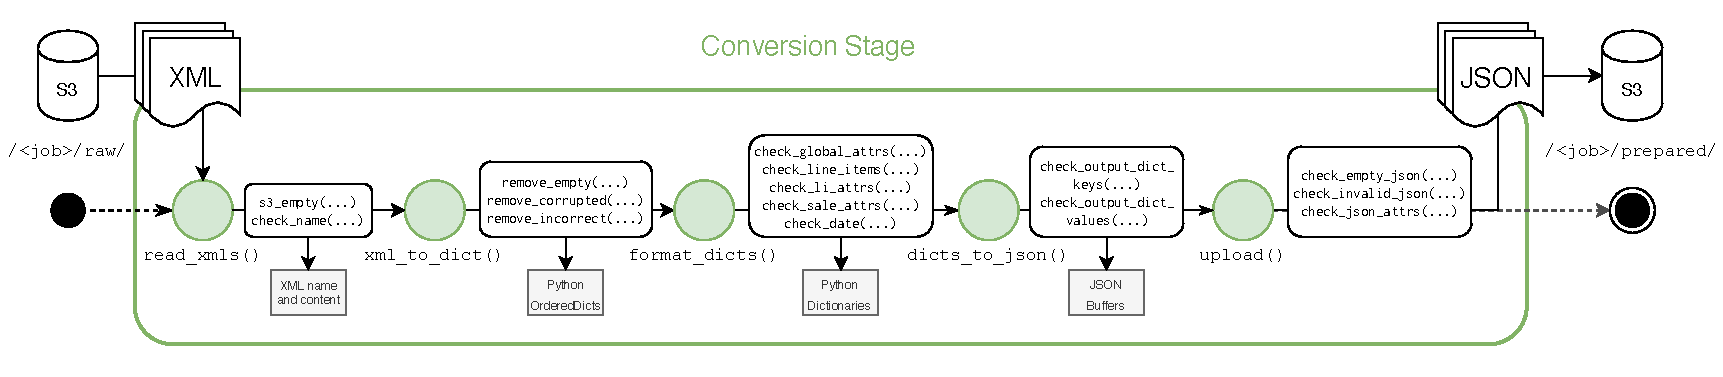
\includegraphics[width=\linewidth]{main-matter/img/5-new-convert}
	\caption{Conversion Stage Overview with Data Handling}
	\label{app:new-convert}
\end{sidewaysfigure}

\end{document}